% !TeX spellcheck = en_US
% !TeX program = pdflatex

\documentclass[12pt,sans]{article}
\usepackage{cmap}
\usepackage[T2A]{fontenc}
\usepackage[utf8]{inputenc}
\usepackage[english]{babel}

%\usepackage{paratype}
\usepackage{PTSans}
\renewcommand{\rmdefault}{\sfdefault}
\usepackage{euler}
\usepackage{ifthen}
\usepackage[most]{tcolorbox}

\usepackage{amsthm,amsmath,amssymb}
\usepackage{xspace}
\usepackage{fullpage}
\usepackage{comment}

%% CALCULATOR
\usepackage{calc}
%% STYLE
\usepackage[dotinlabels]{titletoc}
\usepackage[small]{titlesec}
%% TITLESEC BUG WORKAROUND %%
\usepackage{etoolbox}
\makeatletter
\patchcmd{\ttlh@hang}{\parindent\z@}{\parindent\z@\leavevmode}{}{}
\patchcmd{\ttlh@hang}{\noindent}{}{}{}
\makeatother
%% END %%
\titlelabel{\thetitle.\quad}
%% Puts ``.'' instead of ``:'' in captions
\usepackage{ccaption}
\captiondelim{. }

\usepackage{indentfirst}

\usepackage[mathlines]{lineno}
\linenumbers
%% OTHER

\usepackage[bookmarks=false, colorlinks, unicode, pdfstartview=FitH, pdftex
]{hyperref}
\hypersetup{
 plainpages=true,
 linkcolor=blue,
 citecolor=red,
 menucolor=blue,
 pdfnewwindow=true
}

\usepackage{tikz}
\usetikzlibrary{positioning,calc}

\newcommand{\bits}{\{0,1\}}
\newcommand{\bitstr}{\bits^*}
\newcommand{\sshalf}{{\textstyle\frac12}}
\newcommand{\seqn}[2]{{#1}_1,{#1}_2,\dotsc,{#1}_{#2}}
\newcommand{\seqin}[3]{{#1}_{{#2}_1},{#1}_{{#2}_2},\dotsc,{#1}_{{#2}_{#3}}}
\newcommand{\IC}{\mathrm{IC}}
\newcommand{\poly}{\mathrm{poly}}
\newcommand{\Nat}{\mathbb{N}}

\DeclareMathOperator{\dom}{dom}
\DeclareMathOperator{\rank}{rank}
\DeclareMathOperator{\rng}{rng}
\DeclareMathOperator*{\E}{\mathbb{E}}
\DeclareMathOperator{\KL}{D_{KL}}
\DeclareMathOperator{\CE}{CE}
\newcommand{\midd}{\parallel}



\theoremstyle{definition}
\newtheorem{definition}{Definition}[section]

\theoremstyle{plain}
\newtheorem{theorem}{Theorem}[section]
\newtheorem{lemma}{Lemma}[section]
\newtheorem{statement}{Statement}[section]
\newtheorem{corollary}{Corollary}[section]

\theoremstyle{remark}
\newtheorem{example}{Example}[section]
\newtheorem{exercise}{Exercise}[section]
\newtheorem{remark}{Remark}[section]
\newtheorem{problem}{Problem}[section]

\newboolean{forstudents}
\setboolean{forstudents}{false}

\definecolor{block-gray}{gray}{.9}
\newtcolorbox{solutionblock}{colback=block-gray,grow to right by=-10mm,grow to left by=-10mm,
    boxrule=0pt,boxsep=0pt,breakable}

\ifthenelse{\boolean{forstudents}}{\excludecomment{solution}}{%
\newenvironment{solution}{%
    \begin{solutionblock}\emph{Solution.}
    }{%
    \end{solutionblock}
}}


\newenvironment{tasks}{\paragraph{Problems.}\begin{enumerate}}{\end{enumerate}}

%opening
\title{Notes on Information Theory}
\author{Alexander V. Smal}
\begin{document}

\maketitle

\begin{abstract}
    This course is dedicated to studying approaches to defining the concept of ``quantity of information''. The sequence of material presentation is based on Kolmogorov's classic article ``Three Approaches to the Definition of the Concept of Quantity of Information'' (1965).

    The course will cover three approaches to defining ``quantity of information'':
    \begin{itemize}
        \item Combinatorial (information by Hartley)
        \item Probabilistic (Shannon entropy)
        \item Algorithmic (Kolmogorov complexity)
    \end{itemize}

    In addition, we will discuss various applications of information theory in different fields of computer science: in cryptography, communication complexity, coding theory, finite automata theory, computational complexity theory, and others.
\end{abstract}

\newpage\tableofcontents\newpage

\section{Combinatorial Approach}
\subsection{Hartley's definition}
Let a finite set \(A\) be given—\emph{the set of outcomes}.
\begin{definition}[1928]
    We define \emph{the amount of information in \(A\)} as \(\chi(A) = \log_{10}|A|\).
\end{definition}

According to this definition a set of size 10 has 1 unit of information.
Note that the base of algorithm can be different.

If it becomes known for some \(x\in A\) that \(x\in B\), then to identify \(x\) we now need \(\chi(A\cap B) = \log |A\cap B|\) bits, i.e., we have been informed \(\chi(A) - \chi(A\cap B)\) bits of information.

\begin{example}
    Suppose we want to discover some unknown ordering of the set $\{\seqn{a}{5}\}$. We have learned that \(a_1>a_2\) or \(a_3>a_4\). How many bits of information have we gained? The set \(A\) consists of \(5!\) permutations, while the set \(B\) consists of the permutations that satisfy the new condition. It is easy to verify that \(|B| = 90\). Thus, we have learned \(\log 120 - \log 90 = \log(4/3)\) bits.
\end{example}

Let \(A\subset\bitstr\times\bitstr\). Denote by \(\pi_1(A)\) and \(\pi_2(A)\) the projections of the set \(A\) onto the first and second coordinates, respectively, and let \(\chi_1(A) = \log|\pi_1(A)|\) and \(\chi_2(A) = \log|\pi_2(A)|\) be the quantity of information in them according to Hartley.

\begin{theorem}
    \(\chi(A) \le \chi_1(A) + \chi_2(A)\).
\end{theorem}

\begin{definition}
    The quantity of information in the second coordinate of \(A\subset\bitstr\times\bitstr\) given the first is
    \[\chi_{2|1} = \log\max_{a\in\pi_1(A)}\bigl|\{x \mid (a, x)\in A\}\bigr|.\]
\end{definition}

\begin{theorem}
    \(\chi(A) \le \chi_1(A) + \chi_{2|1}(A)\).
\end{theorem}

\begin{theorem}\label{thm:volume}
    For \(A\subset\bitstr\times\bitstr\times\bitstr\)
    \[2\cdot\chi(A) \le \chi_{12}(A) + \chi_{13}(A) + \chi_{23}(A).\]
\end{theorem}
\begin{corollary}
    The square of the volume of a three-dimensional body does not exceed the product of the areas of its projections onto the coordinate planes.
\end{corollary}

\begin{statement}
    If \(f: X\to Y\)
    \begin{enumerate}
        \item is a surjection, then \(\chi(Y)\le \chi(X)\),
        \item is an injection, then \(\chi(X)\le \chi(Y)\).
    \end{enumerate}
\end{statement}

\subsection{Application: The Game of 10 Questions}
How many yes/no questions need to be asked to determine a secret number from 1 to \(N\), if (a) questions can be asked adaptively; (b) questions must be written down in advance.

The estimate \(\lceil\log N\rceil\) is achieved in both cases if questions about the bits of the binary representation of the secret number are asked.

Let's prove the lower bound. Let \(A=[N]\). The set \(Q = \{(\seqn{q}{k})\}\) is the set of protocols (answers to the questions). We can consider \(A\) and \(Q\) as projections of some outcome set of the game \(S\) onto different coordinates. Then the following inequalities hold:
\begin{itemize}
    \item \( \chi_Q(S) = \chi(Q) \le \chi_1(Q) + \chi_2(Q) + \dotsb + \chi_k(Q) \le k, \)
    \item \( \chi_A(S) = \chi(A) \le \chi(S) \le \chi_Q(S) + \chi_{A|Q}(S) \le k + 0 = k. \)
\end{itemize}
Thus, we obtain \(\log N = \chi(A) \le k\).

\subsection{Cost of Information}
Let a secret integer be chosen from 1 to \(n\) (where \(n \ge 2\)).
Any yes/no questions can be asked. For a positive answer, we will pay 1 ruble, and for a negative answer—two rubles. How much is necessary and sufficient to guess the number?

\paragraph{Upper Bound.} We will ask questions in such a way that negative answers provide twice as much information as positive ones. Then for each bit of information, we will pay a constant amount of rubles \(c\). Let all questions be of the form “is \(x \in T\)?”. We require that
\[2\cdot(\log |X| - \log|X \cap T|) = \log |X| - \log|X\cap\overline T|.\]
Let \(|X \cap T| = \alpha|X|\), then \(|X\cap\overline T| = (1 - \alpha)|X|\),
thus we obtain the equation
\[2\log (1/\alpha) = \log (1/(1-\alpha)),\]
equivalent to the quadratic equation
\[\alpha^2 = 1 - \alpha.\] Among the two roots, we are interested in the one that is less than 1, i.e., \(\alpha=(\sqrt 5 - 1) / 2\). Therefore, for any answer, we will pay \(c = 1/(-\log \alpha)\approx 1.44\) rubles per bit, and in total—\(c\log n\) rubles.

In this estimate, we have completely ignored rounding questions. Indeed, we can never divide a set of \(n\) elements into two in the ratio \(\alpha:(1-\alpha)\), since \(\alpha\) is irrational. Therefore, some rounding error will accumulate with each question. Instead of questions about membership in a certain subset \(T\) of the set \(X\), let's ask about membership in an interval with real coordinates. We start with the interval \(S = [1,n]\) and will reduce it by a factor of \(1/\alpha\) each time, i.e., we will first ask whether \(x\) belongs to the interval \(S' = [1, 1 + \alpha(n-1)]\). The length of the interval \(S'\) is \(1/\alpha\) times less than the length of the interval \(S\). We will continue in this manner until the length of the interval becomes less than 1—in this case, \(x\) is uniquely defined. After each question, the length of the interval decreases at most by a factor of \(1/(1 - \alpha) = 1/\alpha^2\), so the length of the last interval is at least \(\alpha^2\). Thus, the length of the interval will not reduce by more than \((n-1)/\alpha^2\) times. Since we chose the intervals each time so that we pay \(c\) rubles for a decrease of \(\log |S|\) by 1, we will pay in total no more than
\[
c\log((n-1)/\alpha^2) = c\log(n-1) - 2c\log \alpha = c\log(n-1) + 2.
\]
In any outcome, we will pay a whole number of rubles, so this estimate can be refined to \(\lfloor c\log(n-1)\rfloor + 2\).

\paragraph{Lower Bound.} We will apply the adversary argument. Let the adversary
choose the answer YES/NO depending on which of the two values \(1/(\log |X| - \log|X \cap T|)\) and \(2/(\log |X| -
\log|X \cap \overline T|)\) is greater. For any \(X,\ T\), one of these values is at least \(c = 1/(-\log\alpha)\). Thus,
we force the algorithm to pay at least \(c\) rubles per bit, meaning that any algorithm in the worst case will pay
\(\lceil c\log n\rceil\) rubles.

\subsection{Application: Sorting Stones by Weight}
\subsubsection{Upper and Lower Bounds for Arbitrary \(N\)}
How many comparisons are needed to sort \(N\) stones by weight?

\paragraph{Lower Bound.} It will require \(\lceil\chi(S_N)\rceil = \lceil\log n!\rceil\) comparisons.

\paragraph{Upper Bound.} We will sort using insertion sort with binary search for the insertion point. The number of comparisons is:
\[
\lceil\log 2\rceil + \lceil\log 3\rceil + \dotsb + \lceil\log n\rceil \le \log n! + n - 1 = n\log n + O(n).
\]

\subsubsection{Exact Estimates for Small \(N\)}
\begin{exercise}
    How many weighings are needed to sort \(N\) stones by weight?
    Find the exact answer to this question for \(N = 2, 3, 4, 5\). Hint: use a greedy strategy where each weighing provides maximum information.
\end{exercise}

\subsection{Application: Finding the Fake Coin}
The following problems are proposed.
\begin{itemize}
    \item There are 20 visually identical coins, one of which is fake and lighter than the others.
    How can you find the fake coin using a balance scale? What is the minimum number of weighings needed?

    \textit{Solution.} Each weighing provides at most \(\log 3\) bits of information, so the number of weighings is at least $\lceil\log 20 / \log 3\rceil = \lceil\log_3 20\rceil = 3$.

    \item There are 13 visually identical coins, one of which is fake (with unknown relative weight).
    Can you find the fake coin and determine its relative weight in three weighings?

    \begin{solution}
        We need to consider two options for the first step:
    \begin{itemize}
        \item If we weigh 4 coins, then if they are equal, we cannot find the fake coin among 5 in two weighings (10 outcomes remain),
        \item If we weigh 5 coins, then if they are unequal, 10 possible outcomes remain.
    \end{itemize}
    \end{solution}

    \item There are 15 visually identical coins, one of which is fake. Can you find the fake coin in three weighings
    if you do not need to determine its relative weight?

    \textit{Solution.} Let's consider how many different outcomes there can be. The only case in which we can identify the fake coin without knowing its relative weight is if it has never been on the scale. This means that in all three weighings, the scale will be balanced. Therefore, there can be only one such coin, and in other cases, we will know the relative weight. In such a case, the number of different outcomes is \(2\cdot 14 + 1 = 29\), which exceeds \(3^3\)~— the number of results of three weighings.

    \item There are 14 visually identical coins, one of which is fake. Can you find the fake coin in three weighings
    if you do not need to determine its relative weight?

    \textit{Instead of a solution.} Similar reasoning does not allow proving impossibility, since \(2\cdot 13 + 1 = 3^3\).
    Nevertheless, it is impossible to solve this problem in three weighings. To prove this, we need more than
    the definition of information by Hartley.

\end{itemize}

\begin{exercise}
    Find one fake coin among 12 in three weighings, if its relative weight is unknown. Hint: use a ``greedy'' strategy, where each weighing provides maximum information.
\end{exercise}

\begin{exercise}
    Let \(L_n\) be the set of paths of length \(n\) in a graph.
    \begin{center}
        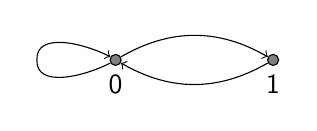
\begin{tikzpicture}
            \tikzstyle{vert}=[circle, draw, fill=black!50,
            inner sep=0pt, minimum width=4pt]
            \node[vert, label=below:0] (a) at (1,0) {};
            \node[vert, label=below:1] (b) at (3,0) {};
            \node (c) at (0,0) {};
            \path
            (a) edge [->,bend left] (b)
            (b) edge [->,bend left] (a)
            (a) edge [bend left, in=90] (0,0)
            (0,0) edge [->,bend left,out=90] (a);
        \end{tikzpicture}
    \end{center}
    What is the limit \(\lim_{n\to\infty} \frac{\chi(L_n)}{n}\)?
\end{exercise}

\begin{exercise}
    Let a number be chosen from 1 to \(N\). You can ask any yes/no questions. How many questions will be needed if one answer can be incorrect, and the questions (a) can be asked adaptively; (b) need to be written in advance?
\end{exercise}

\subsection{Logic of Knowledge}
In this section, we will refer to a set of outcomes \(A\) as a set of \emph{worlds}.
Let \(f\) be some function from \(A\) to a set \(I\) (we will perceive this as information about the world).
We are not concerned with the specific values that \(f\) takes; rather, we will focus on the equivalence classes into which \(f\) divides \(A\):
each equivalence class will consist of worlds in \(A\) with the same value of \(f\).

\begin{example}
    Let \(A = \{1,2,3,4,5\}\), and \(f(x) = x \bmod 3\). Then \(f\) divides \(A\) into three equivalence classes
    \(\{1,4\}\), \(\{2,5\}\), and \(\{3\}\).
\end{example}

Let \(B \subset A\) be some \emph{statement} about the worlds. \(B\) is \emph{true} in world \(x\) if \(x \in B\).
Otherwise, \(B\) is \emph{false} in \(x\). In world \(x\), we \emph{know that \(B\) is true} if \(y \in B\) for all
\(y \sim x\).

\begin{example}
    Let \(A = \{1,2,3,4,5\}\), and \(f(x) = x \bmod 3\). Then in worlds \(1\), \(4\), and \(3\) we know that the world is less than \(5\).
    In worlds \(2\) and \(5\) we do not know.
\end{example}
\begin{remark}
    By ``not knowing,'' we will mean ``it is not true that we know.''
\end{remark}

Common logical connectives can be applied to statements about worlds: ``AND'' (intersection), ``OR'' (union),
``NOT'' (complement).

\begin{statement}
    If in world \(x\) we know \(B\), then in world \(x\) we know that we know \(B\).
    Similarly, if in world \(x\) we do not know \(B\), then in world \(x\) we know that we do not know \(B\).
\end{statement}

Now suppose we have \(k\) people with their own knowledge about the world.
They define \(k\) equivalence relations \(\sim_1, \sim_2, \dotsc, \sim_k\) and,
accordingly, \(k\) partitions into equivalence classes.

\begin{example}
    Let the set of worlds \(A = \{1,2,3,4,5\}\) and there are two people, Alice and Bob.
    Alice knows the values \(f_A(x) = x \bmod 3\), while Bob knows \(f_B(x) = x \bmod 2\).
    Then Alice's equivalence classes are: \(\{1,4\}\), \(\{2,5\}\), and \(\{3\}\),
    while Bob's equivalence classes are: \(\{1,3,5\}\) and \(\{2,4\}\).
    In world 1, Alice knows that the world is less than 5, while Bob does not know. In world 4, both know this.
    In world 1, Alice does not know that Bob does not know that the world is less than 5 (indeed, in world 4,
    which is equivalent to 1 from Alice's perspective, Bob knows this).
\end{example}

\begin{exercise}
    Suppose there is a card known to have a non-negative integer \(n\) written on one side and the integer \(n+1\) on the other side.
    Alice and Bob are sitting opposite each other, looking at this card from different sides, and the following conversation occurs between them.
    \begin{itemize}
        \item[A:] I do not know the number on Bob's side.
        \item[B:] I do not know the number on Alice's side.
    \end{itemize}
    This is repeated 10 times, after which Alice says that she knows the number on Bob's side. What numbers could have been written on the card?
\end{exercise}

\begin{exercise}
    In a shop, there are three red hats and two white hats. Three gentlemen take turns buying a random hat and putting it on without looking
    (i.e., the gentleman does not know the color of the hat he bought). After this, the gentlemen look at each other and the following conversation occurs.
    \begin{itemize}
        \item[1:] I do not know the color of my hat.
        \item[2:] I do not know the color of my hat.
        \item[3:] Now I know the color of my hat.
    \end{itemize}
    What color is the hat on the third gentleman?
\end{exercise}

\begin{exercise}
    The king has 9 bottles of wine. One of the bottles contains poisoned wine.
    The king has two maids. Each day, any maid can mix a cocktail from different bottles in her glass and drink it, but each maid only gets one attempt per day, at a fixed time, exactly at noon (so if both maids try, one cannot take the result of the other into account on the same day). Any amount of poisoned wine in the glass will quickly kill.

    How can one discover which bottle is poisoned in two days?
\end{exercise}

\section{Probabilistic Approach}
\subsection{Shannon Entropy}

Shannon entropy defines the amount of information \(H(\alpha)\) in the probability distribution for a random variable \(\alpha\). Let \(\alpha\) take values from the set \(\{\seqn{a}{k}\}\) with probabilities \(\{\seqn{p}{k}\}\), where \(p_i \ge 0\) and \(\sum_i p_i = 1\).

We would like this definition to be consistent with Hartley's definition, i.e., the following ``boundary conditions'' hold:
\begin{itemize}
    \item if \(p_1 = \dotsb = p_k\), then \(H(\alpha) = \log k\),
    \item if \(p_1 = 1\), \(p_2 = \dotsb = p_k = 0\), then \(H(\alpha) = 0\).
\end{itemize}
We will seek \(H(\alpha)\) in the form of the expected value of the information we obtain from each outcome.
\[
H(\alpha) = \sum_i p_i \cdot \text{(information in $a_i$)}.
\]
How do we estimate how much information is in the outcome $a_i$? Let $U$ be the entire space of elementary outcomes, all of which are equally probable. Then, the event \(\alpha = a_i\) corresponds to a set of elementary outcomes with measure \(p_i\). Accordingly, if the event \(\alpha = a_i\) occurs, the size of the set corresponding to this event decreases from \(|U|\) to \(p_i |U|\), i.e., the event \(\alpha = a_i\) tells us \(\log |U| - \log (p_i |U|) = \log \frac{1}{p_i}\) bits of information.

Now let us assume the elementary outcomes are not equally probable. In this case, the event \(\alpha = a_i\) provides us with information that reduces the \emph{measure} of the set of possible outcomes by a factor of \(1/p_i\), i.e., we again obtain \(\log 1 - \log p_i = \log \frac{1}{p_i}\). This leads us to the following definition.
\begin{definition}[1948]
    The Shannon entropy of a random variable \(\alpha\) is given by
    \[
    H(\alpha) = \sum_{i=1}^k p_i \cdot \log \frac{1}{p_i}.
    \]
    (For continuity, we define \(0 \cdot \log \frac{0}{0} = 0\).)
\end{definition}

We can derive this relation from Hartley's definition of information in another way. Let \(W_n\) be the set of all words of length \(n\) consisting of letters \(\{\seqn{a}{k}\}\), where each letter \(a_i\) appears exactly \(n_i = p_i \cdot n\) times (we will assume that the probabilities \(p_i\) are rational, and that the set \(W_n\) is defined only when all \(n_i\) are integers). The information according to Hartley in \(W_n\) is given by
\[
\chi(W_n) = \log |W_n| = \log \frac{n!}{n_1! n_2! \dotsb n_k!}.
\]
This expression can be estimated using Stirling's formula.
\[
\begin{aligned}
    \chi(W_n) & = \log \frac{\poly(n) \cdot (n/e)^n}
    {\poly(n) \cdot (n_1/e)^{n_1} \cdot (n_2/e)^{n_2} \dotsm (n_k/e)^{n_k}} = \\
    & = \log \left(\left(\frac{n}{n_1}\right)^{n_1} \cdot
    \left(\frac{n}{n_2}\right)^{n_2} \dotsm
    \left(\frac{n}{n_k}\right)^{n_k}\right) + O(\log n) = \\
    & = \log \left(\left(\frac{1}{p_1}\right)^{p_1 \cdot n} \cdot
    \left(\frac{1}{p_2}\right)^{p_2 \cdot n} \dotsm
    \left(\frac{1}{p_k}\right)^{p_k \cdot n}\right) + O(\log n) = \\
    & = n \cdot \sum_{i=1}^k p_i \cdot \log \frac{1}{p_i} + O(\log n).
\end{aligned}
\]
On average, there are \(\chi(W_n)/n\) bits of information per symbol. In the limit, we obtain
\[
\lim_{n \to \infty} \frac{\chi(W_n)}{n} = \sum_{i=1}^k p_i \cdot \log \frac{1}{p_i} = H(\alpha)
\]
(the limit should be taken over an infinite subsequence of natural numbers \(n\) such that all \(\{n_i\}\) are integers).

\begin{lemma}\label{lm:entropy-properties}
    The following relations hold for Shannon entropy.
    \begin{itemize}
        \item \(H(\alpha) \ge 0\), and \(H(\alpha) = 0\) \(\iff\) the distribution of \(\alpha\) is degenerate.

        \item \(H(\alpha) \le \log k\), and \(H(\alpha) = \log k\) \(\iff\) the variable \(\alpha\) is uniformly distributed.

    \end{itemize}
\end{lemma}

To prove this, we will need the following theorem.

\begin{theorem}[Jensen's Inequality]
    Let the function \(f(x)\) be concave on some interval \(\mathcal{X}\) and let the numbers \(\seqn{q}{n} > 0\) be such that \(q_1 + \dotsb + q_n = 1\). Then for any \(\seqn{x}{n}\) from the interval \(\mathcal{X}\), the inequality holds:
    \[
    \sum_{i=1}^{n} q_{i} f(x_{i}) \leq f\left(\sum_{i=1}^{n} q_{i} x_{i}\right).
    \]
\end{theorem}

\begin{proof}[Proof of Lemma~\ref{lm:entropy-properties}]
    The first property follows directly from the definition: each term in the sum \(H(\alpha)\) is non-negative and equals zero if and only if \(p_i = 0\) or \(p_i = 1\).

    To prove the second inequality, we will move everything to the left side and apply Jensen's inequality:
    \[
    H(\alpha) - \log k
    = \sum_{i=1}^k p_i \cdot \log \frac{1}{p_i} - \sum_{i=1}^k p_i \cdot \log k
    = \sum_{i=1}^k p_i \cdot \log \frac{1}{p_i k}
    \le \log\left(\sum_{i=1}^k p_i \frac{1}{p_i k}\right) = \log 1 = 0.
    \]
\end{proof}

We denote the entropy of the joint distribution of the pair of random variables \(\alpha\) and \(\beta\) as \(H(\alpha, \beta)\).
\begin{lemma}
    The following properties hold:
    \begin{itemize}
        \item \(H(\alpha, \beta) \le H(\alpha) + H(\beta)\), with equality occurring if and only if the random variables are independent;
        \item \(H(\alpha) \le H(\alpha, \beta)\), with equality occurring if and only if \(\beta\) is completely determined by the value of \(\alpha\), i.e., \(\beta = f(\alpha)\).
    \end{itemize}
\end{lemma}

\begin{proof}
    Let us introduce notations for the probabilities of events in the joint distribution of probabilities \((\alpha, \beta)\). Let the pair \((a_i, b_j)\) have probability \(p_{i,j}\), the event \([\alpha = a_i]\) have probability \(p_{i,*} = p_{i,1} + \dotsb + p_{i,n}\), and the event \([\beta = b_j]\) have probability \(p_{*,j} = p_{1,j} + \dotsb + p_{k,j}\). In these notations, the inequality \(H(\alpha, \beta) \le H(\alpha) + H(\beta)\) can be rewritten as
    \[
    \sum_{i,j} p_{i,j} \cdot \log \frac{1}{p_{i,j}} \le
    \sum_{i} \sum_{j} p_{i,j} \cdot \log \frac{1}{p_{i,*}} +
    \sum_{j} \sum_{i} p_{i,j} \cdot \log \frac{1}{p_{*,j}}.
    \]
    Now, we will move everything to the left side and apply Jensen's inequality.
    \begin{multline*}
        \sum_{i,j} p_{i,j} \cdot \log \frac{p_{i,*} \cdot p_{*,j}}{p_{i,j}} \le
        \log\left(\sum_{i,j} p_{i,j} \cdot \frac{p_{i,*} \cdot p_{*,j}}{p_{i,j}}\right) =
        \log\left(\sum_{i,j} p_{i,*} \cdot p_{*,j}\right) = \\
        = \log \Biggl(\biggl(\underbrace{\sum_{i} p_{i,*}}_1\biggr) \cdot
        \biggl(\underbrace{\sum_{j} p_{*,j}}_1\biggr)\Biggr) = 0.
    \end{multline*}

    Equality in Jensen's inequality for \(f(x) = \log(x)\) occurs only when all points are equal, i.e., for any \(i,j\), \(\frac{p_{i,*} p_{*,j}}{p_{i,j}} = c\) for some constant \(c\). It is easy to see that \(c = 1\), because the following equality holds \(\sum_{i,j} {p_{i,*} p_{*,j}} = c \sum_{i,j} {p_{i,j}}\), in which both sums equal 1. Thus, in the case of equality, \(\alpha\) and \(\beta\) are independent.

    The proof of the second property will follow from the properties of conditional entropy.
\end{proof}


\begin{definition}\label{def:cond-entropy1}
    The entropy of \(\alpha\) given \(\beta = b_j\) is defined as
    \[
    H(\alpha\mid\beta = b_j) = \sum_i \Pr[\alpha = a_i\mid \beta = b_j] \cdot
    \log\frac{1}{\Pr[\alpha = a_i\mid \beta = b_j]}.
    \]
\end{definition}

\begin{definition}\label{def:cond-entropy2}
    The \emph{conditional (relative) entropy} of \(\alpha\) with respect to \(\beta\) is given by
    \[
    H(\alpha\mid\beta) = \sum_j \Pr[\beta = b_j] \cdot H(\alpha\mid \beta = b_j).
    \]
    In other words,
    \[
    H(\alpha\mid\beta) = \E\limits_{b_j \gets \beta}[H(\alpha\mid \beta = b_j)].
    \]
    If we substitute Definition~\ref{def:cond-entropy1}, we can obtain an expression for conditional entropy in terms of individual probabilities of events:
    \[
    H(\alpha\mid\beta) =
    \sum_j \Pr[\beta = b_j] \cdot
    \sum_i \Pr[\alpha = a_i\mid \beta = b_j] \cdot
    \log\frac{1}{\Pr[\alpha = a_i\mid \beta = b_j]}  =
    \sum_{i,j} p_{i,j} \cdot \log\frac{p_{*,j}}{p_{i,j}}.
    \]
\end{definition}

\begin{lemma}
    The conditional entropy has the following properties:
    \begin{itemize}
        \item \(H(\alpha\mid\beta) \ge 0\).
        \item \(H(\alpha\mid\beta) = 0\) \(\iff\) \(\alpha\) is uniquely determined by \(\beta\).
        \item \(H(\alpha,\beta) = H(\beta) + H(\alpha\mid\beta) = H(\alpha) + H(\beta\mid\alpha)\).
    \end{itemize}
\end{lemma}

\begin{proof}
    The first property holds because conditional entropy is the expectation of a non-negative random variable. The second property is explained by the fact that for any \(j\), the distribution \(\langle \alpha \mid \beta = b_j \rangle\) has zero entropy, i.e., the distribution is degenerate and each \(b_j\) corresponds to exactly one \(a_i\). The third property follows from the following equality:
    \[
    \sum_{i,j} p_{i,j} \cdot \log\frac{1}{p_{i,j}} =
    \sum_{i,j} p_{i,j} \cdot \log\frac{1}{p_{*,j}} +
    \sum_{i,j} p_{i,j} \cdot \log\frac{p_{*,j}}{p_{i,j}}.
    \]
    (Care must be taken if there are rows consisting entirely of zeros, i.e., \(p_{*,j} = 0\) — such rows should not be included in these sums.)
\end{proof}

\begin{corollary}
    \(H(\alpha,\beta) \ge H(\alpha)\), with equality occurring if and only if \(\beta = f(\alpha)\).
\end{corollary}

\begin{proof}
    \(H(\alpha,\beta) - H(\alpha) = H(\beta\mid\alpha) \ge 0\). By the second property of conditional entropy, equality occurs if and only if \(\beta = f(\alpha)\).
\end{proof}

\subsection{Mutual Information}

\begin{definition}
    The \emph{information in \(\alpha\) about the variable \(\beta\)} is defined as:
    \[
    I(\alpha:\beta) = H(\beta) - H(\beta\mid\alpha).
    \]
    This quantity is also referred to as the \emph{mutual information of the random variables \(\alpha\) and \(\beta\)}.
\end{definition}

\begin{lemma}
    The following relations hold for mutual information:
    \begin{enumerate}
        \item \(I(\alpha:\beta) \le H(\alpha)\).
        \item \(I(\alpha:\beta) \le H(\beta)\).
        \item \(I(\alpha:\alpha) = H(\alpha)\).
        \item \(I(\alpha:\beta) = I(\beta:\alpha)\).
        \item \(I(\alpha:\beta) = H(\alpha) + H(\beta) - H(\alpha,\beta)\).
    \end{enumerate}
\end{lemma}

\begin{definition}
    Let \(\alpha, \beta, \gamma\) be random variables. We define the \emph{information in \(\alpha\) about \(\beta\) given \(\gamma\)} as follows:
    \begin{enumerate}
        \item \(I(\alpha:\beta\mid\gamma) = H(\beta\mid\gamma) - H(\beta\mid\alpha,\gamma)\).
        \item \(I(\alpha:\beta\mid\gamma) = \sum_\ell I(\alpha:\beta \mid \gamma = c_\ell) \cdot \Pr[\gamma = c_\ell]\).
        \item \(I(\alpha:\beta\mid\gamma) = H(\alpha\mid\gamma) + H(\beta\mid\gamma) - H(\alpha,\beta\mid\gamma)\).
        \item \(I(\alpha:\beta\mid\gamma) = H(\alpha,\gamma) + H(\beta,\gamma) - H(\alpha,\beta,\gamma) - H(\gamma)\).
    \end{enumerate}
\end{definition}

\begin{lemma}
    All definitions of conditional mutual information are equivalent.
\end{lemma}

\begin{proof}
    (3) \(\iff\) (4).
    \[
    (3) = H(\alpha\mid\gamma) + H(\beta\mid\gamma) - H(\alpha,\beta\mid\gamma) =
    H(\alpha,\gamma) - H(\gamma) + H(\beta,\gamma) - H(\gamma) -
    H(\alpha,\beta,\gamma) + H(\gamma).
    \]
\end{proof}

\begin{statement}[Chain rule for mutual information]
    The following relations hold:
    \begin{enumerate}
        \item \(I((\alpha,\beta) : \gamma) = I(\alpha : \gamma) + I(\beta: \gamma \mid \alpha)\).
        \item \(I((\alpha,\beta) : \gamma \mid \delta) = I(\alpha : \gamma \mid \delta) + I(\beta: \gamma \mid \alpha, \delta)\).
    \end{enumerate}
\end{statement}


\subsection{Approachlication: Again on Finding the Fake Coin}
Now we have enough knowledge to prove that it is impossible to find one fake coin out of 14 with just three weighings, even if we do not need to determine its relative weight.

\begin{proof}
    Suppose there exists a way to find the fake coin in three weighings. Then the weighing protocol can be represented as a complete ternary tree, where each leaf is labeled with the number of the coin that turned out to be fake (we have exactly \(3^3 = 27\) outcomes).

    Let us introduce the following probability distribution \(\alpha\). Suppose the coin whose number is at the leaf corresponding to the three equalities (there is only one such leaf) has number \(i\). In our probability distribution, the coin with number \(i\) will be fake with a probability of \(1/27\). The remaining coins turn out to be fake with probabilities of \(2/27\), where with a probability of \(1/27\) the coin is lighter than the genuine one, and with the same probability, it is heavier than the genuine one.
    \[
    H(\alpha) = \log 27 = 3\log 3.
    \]

    Let the random variables \(\beta_1\), \(\beta_2\), \(\beta_3\) correspond to the results of the first, second, and third weighings, respectively. The value of \(\alpha\) is uniquely determined after three weighings:
    \[
    H(\alpha\mid\beta_1,\beta_2,\beta_3) = 0,
    \]
    and therefore
    \[
    H(\alpha) \le H(\beta_1,\beta_2,\beta_3) \le H(\beta_1) + H(\beta_2) + H(\beta_3) \le 3\log 3.
    \]
    Thus, each weighing must have an entropy of exactly \(\log 3\).

    Consider the first weighing. Let there be \(k\) coins on each side of the scale. The probability of each outcome of the weighing (\(<\), \(>\), \(=\)) with respect to the distribution \(\alpha\) must be exactly \(1/3\).
    \[
    \Pr[<] = \frac{k}{27} + \frac{k}{27} = \frac{1}{3}.
    \]
    Thus, \(2k = 9\), which means there is no such integer \(k\).
\end{proof}

\begin{exercise}
    Suppose we have \(N\) stones of different weights and a balance scale. How many weighings are needed to find
    \begin{enumerate}
        \item the heaviest and the second heaviest stone,
        \item the heaviest and the lightest stones.
    \end{enumerate}
\end{exercise}


\section{Codes}
\subsection{Uniquely Decodable Codes}
\begin{definition}
    We will call a \emph{code} a function \(C:\{\seqn{a}{n}\}\to\bitstr\),
    which assigns \emph{codewords} to the letters of a certain alphabet.
    If any message obtained by applying the code \(C\) can be decoded
    uniquely (i.e., it can only be segmented into images of \(C\) in one way),
    then such a code is called \emph{uniquely decodable}.
\end{definition}

\begin{definition}
    A code is called \emph{prefix (prefix-free)}, if no
    codeword is a prefix of another codeword.
\end{definition}

\begin{theorem}[Kraft-McMillan Inequality]\label{thm:mcmill}
    For any uniquely decodable code with a set of codewords
    \(\{\seqn{c}{n}\}\), the following inequality holds:
    \[
    \sum_{i=1}^{n} 2^{-|c_i|} \le 1.
    \]
\end{theorem}

\begin{lemma}
    The Kraft-McMillan inequality holds for prefix codes.
\end{lemma}

\begin{proof}
    Consider the tree of the prefix code and calculate the total measure of the subtrees
    corresponding to the codewords.
\end{proof}

\begin{statement}
    For prefix codes, the converse is also true: if there is a set of integers
    \(\{\seqn{\ell}{n}\}\)
    that satisfies the Kraft-McMillan inequality
    \[
    \sum_{i=1}^{n} 2^{-\ell_i} \le 1,
    \]
    then there exists a prefix code with codewords \(\{\seqn{c}{n}\}\), where \(|c_i| = \ell_i\).
\end{statement}

\begin{proof}
    Sort \(\ell_i\) in ascending order and place them in an infinite
    binary tree, choosing the leftmost free node
    of the corresponding measure each time. It can be noted that we will always be able to find such a node.
\end{proof}

\begin{corollary}
    For any uniquely decodable code, there exists a prefix code with the same
    lengths of codewords.
\end{corollary}

\begin{proof}[Proof of Theorem~\ref{thm:mcmill}]
    Assign to the codewords \(\{c_i\}\) the monomials \(\{p_i\}\) in the variables \(x\) and \(y\) such
    that each '0' in the codeword corresponds to \(x\), and each '1' corresponds to \(y\):
    \[
    c_i = 0110101 \implies p_i(x,y) = xyyxyxy.
    \]
    Consider the following expression for some \(L\).
    \[
    \left( \sum_{i=1}^n p_i(x,y) \right)^L = \sum_{\ell=L}^{\max|c_i| \cdot L} M_\ell(x,y),
    \]
    where \(M_\ell\) denotes the sum of all resulting monomials of degree \(\ell\).
    Note that in each \(M_\ell\), there are at most \(2^\ell\) monomials: otherwise,
    the code would not be uniquely decodable—each monomial (disregarding
    commutativity and associativity) could be obtained at most once.

    Now consider the value of this expression at \(x = y = \frac{1}{2}\).
    \begin{equation}\label{eq:kraftproof}
        \left( \sum_{i=1}^n p_i\bigl(\sshalf,\sshalf\bigr) \right)^L =
        \sum_{\ell=L}^{\max|c_i| \cdot L} M_\ell\bigl(\sshalf,\sshalf\bigr) \le
        \sum_{\ell=L}^{\max|c_i| \cdot L} (2^{-\ell} \cdot 2^\ell) =
        L\cdot\max|c_i| = O(L).
    \end{equation}

    Now assume that the Kraft-McMillan inequality does not hold, i.e.
    \[
    q = \sum_{i=1}^n p_i(1/2,1/2) = \sum_{i=1}^n 2^{-|c_i|} > 1.
    \]
    Comparing this with \eqref{eq:kraftproof}, we obtain a contradiction:
    \(
    q^L = O(L)
    \)
    (the left side grows exponentially, while the right side grows linearly).
\end{proof}

Let \(p_i\) be the probability assigned to each symbol of the alphabet. We will be
interested in the shortest average codes, i.e., those that minimize
\[
\sum_{i=1}^n p_i \cdot |c_i| \to \min.
\]
\begin{theorem}[Shannon]
    For any uniquely decodable code, the following holds:
    \[
    \sum_{i=1}^n p_i \cdot |c_i| \ge \sum_{i=1}^n p_i \cdot \log \frac{1}{p_i}.
    \]
\end{theorem}
\begin{proof}
    We will move everything to the right side and apply Jensen's inequality:
    \[
    \sum_{i=1}^n p_i \cdot \log \frac{2^{-|c_i|}}{p_i} \le
    \log \sum_{i=1}^n \left(p_i \frac{2^{-|c_i|}}{p_i}\right) =
    \log \sum_{i=1}^n 2^{-|c_i|} \le \log 1 = 0.
    \]
\end{proof}

\begin{theorem}[Shannon]\label{thm:shannon:optcode}
    For any probability distribution \(\{\seqn{p}{n}\}\), there exists
    a uniquely decodable/prefix code \(\{\seqn{c}{n}\}\) such that
    \[
    \sum_{i=1}^n p_i \cdot |c_i| \le \sum_{i=1}^n p_i \cdot \log \frac{1}{p_i} + 1.
    \]
\end{theorem}
\begin{remark}
    The '+1' on the right side cannot be eliminated: for example, if we have only two symbols in
    the alphabet, then \(\sum p_i \cdot |c_i| = 1\), while \(\sum
    p_i \log \frac{1}{p_i}\) can be arbitrarily close to zero.
\end{remark}

\begin{proof}
    We will show that there exists \(\{\seqn{c}{n}\}\) such that \(|c_i| =
    \bigl\lceil \log \frac{1}{p_i} \bigr\rceil\). The code exists because the lengths \(c_i\) satisfy
    the Kraft-McMillan inequality:
    \[
    \sum_{i=1}^n 2^{-|c_i|} =
    \sum_{i=1}^n 2^{-\lceil \log \frac{1}{p_i} \rceil} \le
    \sum_{i=1}^n 2^{-\log \frac{1}{p_i}} =
    \sum_{i=1}^n p_i = 1.
    \]
    Now we estimate the average length of the code:
    \[
    \sum_{i=1}^n p_i \cdot |c_i| =
    \sum_{i=1}^n p_i \cdot \bigl\lceil \log{\textstyle\frac{1}{p_i}} \bigr\rceil <
    \sum_{i=1}^n p_i \cdot \bigl(\log{\textstyle\frac{1}{p_i}} + 1\bigr) =
    \left(\sum_{i=1}^n p_i \cdot \log{\textstyle\frac{1}{p_i}}\right) + 1. \qedhere
    \]
\end{proof}

\subsection{Shannon-Fano Code}
We will sort the probabilities of the symbols in descending order: \(p_1 \ge p_2 \ge \dotsb \ge p_n\).
We will place segments of lengths \(p_1\), \(p_2\), \ldots, \(p_n\) on a line without gaps,
denoting the \(i\)-th segment as \(S_i\), and their union as \(S\).
The codes for the letters \(a_i\) for which the segment \(S_i\) falls in the left half of \(S\)
will begin with '0', while the codes for those letters for which the segment \(S_i\) falls
in the right part of \(S\) will begin with '1'. The central segment may not fall entirely
into one of the halves of \(S\). If the central segment is the first
or last, we will start its code with '0' or '1', respectively.
Otherwise, we will assign it to either half of \(S\) arbitrarily. We then
apply this strategy separately to the letters in the left half of \(S\) and separately for
the right half of \(S\). We repeat this until we obtain unique codes for all
symbols.

\begin{definition}
    A code is \emph{balanced} if for some constant \(c\) and for
    all \(i\), the following holds: \(|c_i| \le - \log p_i + c\).
\end{definition}

\begin{theorem}[Shannon]
    The average length of the Shannon-Fano code is close to the entropy but is not necessarily
    optimal:
    \[
    \sum_{i=1}^n p_i \cdot |c_i| = H + O(1).
    \]
\end{theorem}
\subsection{Huffman Code}
\begin{definition}
    We will construct the \emph{Huffman code} by induction. For \(n = 2\), the codes are \(c_1 = \langle0\rangle\), \(c_2 = \langle1\rangle\). For \(n > 2\), we will assume that the probabilities are ordered in descending order \(p_1 \ge p_2 \ge \dotsb \ge p_n\). We replace the symbols \(a_{n-1}\) and \(a_n\) with a new symbol \(a_{n-1}'\) with probability \(p_{n-1}' = p_{n-1} + p_n\). We then construct the Huffman code for \(n-1\) symbols. For the symbols \(a_{n-1}\) and \(a_n\), we take the codes \(c_{n-1} = c_{n-1}'0\) and \(c_{n} = c_{n-1}'1\).
\end{definition}

\begin{lemma}
    The average length of a codeword for the Huffman code is optimal; that is, it does not exceed the average length of any other prefix code (and thus any uniquely decodable code).
\end{lemma}

\begin{corollary}
    For the Huffman code, the inequality from Shannon's theorem~\ref{thm:shannon:optcode} holds.
\end{corollary}

\begin{remark}
    The entropy of a random variable can sometimes be conveniently viewed as the average length of the Huffman code.
\end{remark}

\subsection{Block Coding}
To mitigate the unavoidable '+1' in the average code length, we will encode not individual symbols, but blocks of symbols.
Let each block consist of \(k\) symbols. Let the random variables \(\seqn{\alpha}{k}\) be distributed as \(\alpha\) and correspond to the letters in the block.
\[
H(\seqn{\alpha}{k}) = \sum_{i=1}^k H(\alpha_i) = k \cdot H(\alpha).
\]
Then, by Shannon's theorems, we obtain the following bound on the average length of a code for a symbol in the block:
\[
H(\alpha) \le (\text{average length of the letter code in the block}) \le H(\alpha) +
\frac{1}{k}.
\]
When coding blocks of length 100, we achieve a deviation from entropy of no more than 0.01. However, we cannot apply the Huffman code since the algorithm for its construction would require passing \(n^{100}\) frequencies of the symbols.

\subsection{Arithmetic Coding}
We will construct a code with the following bound on the average length:
\[
\sum_{i=1}^n p_i \cdot |c_i| \le \sum_{i=1}^n p_i \cdot \log \frac{1}{p_i} + 2,
\]
which is worse than in Shannon's theorem.

\begin{definition}
    We will call a half-interval \emph{standard} if it has the form
    \([0.v0_2, 0.v1_2)\), where \(v\) is some sequence of bits,
    and the numbers are expressed in binary notation. We will assign to each
    standard interval \([0.v0_2, 0.v1_2)\) the code \(v0\).

    For the first letter of the code on the interval \([0,1]\), we will mark non-overlapping intervals of length
    \(p_i\) from left to right. Let the first letter of the block be \(a_{i_1}\); then for the second letter of the code, we will repeat this operation within the interval corresponding to \(p_{i_j}\) (marking non-overlapping intervals), but the lengths of the intervals will now be scaled by the factor
    \(p_i\). We will repeat this operation \(k\) times. The resulting interval will be assigned the code of the largest standard interval that is completely contained within it.
\end{definition}

\begin{statement}
    In the interval \([a,b)\), there will always be a standard interval of length \(2^{-k}\), where
    \(
    \frac{b-a}{4} < 2^{-k} \le \frac{b-a}{2},
    \)
    that is, the length of the code for any interval in arithmetic coding does not exceed \(\log \frac{4}{b-a} = \log \frac{1}{p} + 2\), where \(p\) is the probability of the corresponding block.
\end{statement}

\begin{remark}
    In the case of a Markov chain, it is possible to construct a code with the corresponding conditional probabilities.
\end{remark}

\begin{exercise}
    Let the Markov chain be defined by a graph.
    \begin{center}
        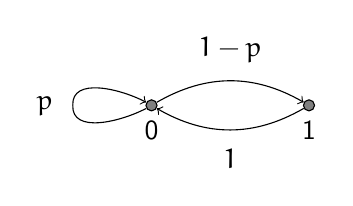
\begin{tikzpicture}
            \tikzstyle{vert}=[circle, draw, fill=black!50,
            inner sep=0pt, minimum width=4pt]
            \node[vert, label=below:0] (a) at (1,0) {};
            \node[vert, label=below:1] (b) at (3,0) {};
            \node (c) at (0,0) {};
            \path
            (a) edge [->,bend left] node[label=above:$1-p$] {} (b)
            (b) edge [->,bend left] node[label=below:$1$]   {} (a)
            (a) edge [bend left, in=90] (0,0)
            (0,0) edge [->,bend left,out=90] (a);
            \node[label=left:$p$] at (0,0) {};
        \end{tikzpicture}
    \end{center}
    Define
    \(
    h_p = \lim_{n\to\infty} \frac{H(\seqn{\alpha}{n})}{n}.
    \)
    Find \(\max\limits_p h_p\).
\end{exercise}

\subsection{Block Codes with Errors}
Let \(\seqn{\alpha}{n}\) be independent identically distributed random variables on \(\{\seqn{a}{k}\}\) with probabilities \(\seqn{p}{k}\). We consider block coding defined by the functions \(E_n\) and \(D_n\):
\[
E_n:\{\seqn{a}{k}\}^n \to \{0,1\}^{L_n},
\]
\[
D_n:\{0,1\}^{L_n} \to \{\seqn{a}{k}\}^n.
\]
\begin{definition}
    The \emph{error probability \(\varepsilon_n\)} is the probability of the following event:
    \[
    [(\seqn{\alpha}{n}) = (\seqin{a}{i}{n}) \mid D_n(E_n(\seqin{a}{i}{n}))\neq (\seqin{a}{i}{n})].
    \]
\end{definition}
\begin{theorem}[Shannon]\label{thm:blockcoding}
    In block coding allowing for errors, the following relations hold:
    \begin{enumerate}
        \item If \(h > H(\alpha) = \sum_{i=1}^{k} p_i \log \frac{1}{p_i}\), then there exist functions \((E_n, D_n)\) for \(L_n = \lceil h \cdot n \rceil\), such that \(\varepsilon_n \to 0\) as \(n \to \infty\).

        \item If \(h < H(\alpha) = \sum_{i=1}^{k} p_i \log \frac{1}{p_i}\), then for any functions \((E_n, D_n)\) for \(L_n = \lceil h \cdot n \rceil\), the error probability \(\varepsilon_n \to 1\) as \(n \to \infty\).
    \end{enumerate}
\end{theorem}
\begin{definition}
    We will say that the word \(w = \langle\seqin{a}{i}{n}\rangle\) is \emph{\(\delta\)-typical} if each letter \(a_j\) occurs in it \(t_j\) times, such that
    \[
    \begin{cases}
        t_j \le (p_j + \delta) \cdot n,\\
        t_j \ge (p_j - \delta) \cdot n.
    \end{cases}
    \]
\end{definition}
\begin{lemma}\label{lm:typicalwordprob}
    For \(\delta = n^{-0.49} = \frac{n^{0.01}}{\sqrt{n}}\), the probability of being not \(\delta\)-typical does not exceed \(\varepsilon_n\), as \(\varepsilon_n \to 0\).
\end{lemma}
\begin{proof}
    Apply Chebyshev's inequality:
    \[
    \mathrm{P}[|X - \mu| \ge \delta n] \le \frac{\sigma^2}{(\delta n)^2} =
    \frac{np_i(1-p_i)}{\delta^2 n^2} = O(n^{-0.02}). \qedhere
    \]
\end{proof}

\begin{lemma}\label{lm:typicalcount}
    For \(\delta = n^{-0.49}\) and \(h > H(\alpha)\), the number of \(\delta\)-typical words does not exceed \(2^{h \cdot n}\) (for sufficiently large \(n\)).
\end{lemma}
\begin{proof}
    First, let us consider words of a specific \emph{type}, in which letter \(i\) occurs \(n_i\) times, with \(n_1 + n_2 + \dotsb + n_k = n\). We will first estimate the number of words of the type where \(n_i = n \cdot p_i\). The number of such words is:
    \[
    \frac{n!}{n_1! n_2! \dotsm n_k!}.
    \]
    By Stirling's formula, \(n! \sim \sqrt{2\pi n}\left(\frac{n}{e}\right)^n \cdot (1 + o(1))\).
    \begin{multline}\label{eq:typicalwords}
        \log \frac{n!}{n_1! n_2! \dotsm n_k!} \approx
        \log \frac{\poly(n) \left(\frac{n}{e}\right)^n}
        {\poly(n)\left(\frac{n_1}{e}\right)^{n_1}\dotsm
            \left(\frac{n_k}{e}\right)^{n_k}} = \\
        = \log \left(\frac{n}{n_1}\right)^{n_1}\dotsm
        \left(\frac{n}{n_k}\right)^{n_k} + O(\log n)
        = \sum_{i=1}^k \underbrace{np_i}_{n_i}\cdot
        \log{\textstyle\frac{1}{p_i}} + O(\log n) < h \cdot n.
    \end{multline}
    The last inequality holds asymptotically, since we assume \(h > H(\alpha)\).
    We have only estimated this for a specific type of words. Now let us estimate for any \(\delta\)-typical word with \(n_i = n \cdot (p_i + \Delta_i)\), where \(|\Delta_i| \le \delta\). Then \eqref{eq:typicalwords} will change as follows:
    \[
    \dots =
    \sum_{i=1}^k n(p_i + \Delta_i) \cdot
    \log{\textstyle\frac{1}{p_i + \Delta_i}} + O(\log n) =
    n \cdot \sum_{i=1}^k p_i \cdot
    \log{\textstyle\frac{1}{p_i}} + O(\log n) + n \cdot O(\delta) < h \cdot n.
    \]
    (Indeed, the entropy is a continuous function, so with a small deviation, it changes by \(c \cdot \max_i \Delta_i\), where \(c\) depends on the derivative of the entropy function.)
    Thus, the total number of \(\delta\)-typical words can be estimated as the number of types multiplied by the number of \(\delta\)-typical words of one type:
    \[
    \poly(n) \cdot 2^{n \cdot H(\alpha) + n \cdot O(\delta) + O(\log n)} < 2^{h \cdot n}. \qedhere
    \]
\end{proof}

\begin{proof}[Proof of Theorem~\ref{thm:blockcoding}] \mbox{}
    \begin{enumerate}
        \item If we code only \(\delta\)-typical words, then by lemma~\ref{lm:typicalcount} it will be sufficient to have code length \(L_n\), and the probability of all non-typical words will tend to zero.

        \item Let \(\hat\varepsilon_n\) be the error probability when decoding \(\delta\)-typical words.
        We want to show that \(\hat\varepsilon_n \to 1\).
        Let us consider a specific \(\delta\)-typical word \(w=\langle\seqin{a}{i}{n}\rangle\). Let \(p_1', p_2', \dotsc, p_k'\) be the frequencies of the letters \(\seqn{a}{n}\) in the word \(w\).
        We estimate the probability of the occurrence of \(w\):
        \[
        \Pr[\langle\seqin{\alpha}{i}{n}\rangle = w] =
        p_1^{p_1' \cdot n} \cdot \dotsc \cdot p_k^{p_k' \cdot n}
        =   2^{-(\sum_i p_i' \log \frac{1}{p_i}) \cdot n}
        \le 2^{-(\sum_i p_i \log \frac{1}{p_i}) \cdot n + O(\delta_n \cdot n)}.
        \]
        In total, we can correctly code no more than \(2^{L_n}\) \(\delta\)-typical words, thus the probability of correctly decoding a \(\delta\)-typical word is
        \[
        1 - \hat\varepsilon_n \le 2^{L_n} \cdot 2^{-H(\alpha) \cdot n + O(\delta_n \cdot n)} \le
        2^{h \cdot n + 1} \cdot 2^{-H(\alpha) \cdot n + O(\delta_n \cdot n)}
        \to 0.
        \]
        Thus, \(\hat\varepsilon_n \to 1\). Together with lemma~\ref{lm:typicalwordprob}, we obtain that \(\varepsilon_n \to 1\). \qedhere
    \end{enumerate}
\end{proof}
\begin{remark}
    Using the previous theorem, one can derive an alternative proof of the inequality \(H(\alpha, \beta) \le H(\alpha) + H(\beta)\). The left side represents the asymptotic average length of the code in block coding \((\alpha, \beta)\), while the right side represents the sum of the average lengths of the codes for \(\alpha\) and \(\beta\) coded separately. Since we can consider coding \((\alpha, \beta)\) as a concatenation of codes for \(\alpha\) and \(\beta\), the inequality holds.
\end{remark}

\section{Properties of Distributions}
\subsection{Entropy Profiles}
\begin{statement}
    For any \(h \ge 0\), there exists a distribution \(\alpha\) such that \(H(\alpha) = h\).
\end{statement}
\begin{proof}
    Take some integer \(n\): \(0 \le h \le \log n\). The desired distribution is a linear combination of the distributions with probabilities \((1, 0, \dotsc, 0)\) and \((\frac{1}{n}, \frac{1}{n}, \dotsc, \frac{1}{n})\).
\end{proof}

What could the joint distribution of two random variables \(\alpha\) and \(\beta\) be? Let us consider how the \emph{entropy profile} \((H(\alpha), H(\beta), H(\alpha, \beta))\) might be structured.

\begin{statement}
    For any numbers \(h_1, h_2, h_{12} \ge 0\) that satisfy the following relations:
\[
    \left\{
    \begin{array}{lll}
        h_{12} \le h_1 + h_2 & \iff & t_0 = I(\alpha:\beta) \ge 0,\\
        h_{2} \le h_{12}     & \iff & t_1 = H(\alpha \mid \beta) \ge 0,\\
        h_{1} \le h_{12}     & \iff & t_2 = H(\beta \mid \alpha) \ge 0.
    \end{array}
    \right.
\]
    there exists a pair of random variables \((\alpha, \beta)\) with the entropy profile \((h_1, h_2, h_{12})\).

\end{statement}
\begin{proof}
    Let \(\xi_0, \xi_1, \xi_2\) be independent random variables with entropies \(t_0, t_1, t_2\) respectively. Then \(\alpha = (\xi_0, \xi_1)\) and \(\beta = (\xi_0, \xi_2)\) will be the desired variables.
    \begin{center} \mbox{}\hfill
    \parbox{.4\textwidth}{\centering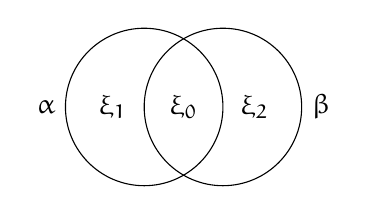
\begin{tikzpicture}
    \tikzstyle{circ}=[circle, draw, inner sep=0pt, minimum width=2cm]

    \node[circ, label=left:$\alpha$] (a) at (0,0) {};
    \node[circ, label=right:$\beta$] (b) at (1,0) {};
    \node at (-.4,0) {$\xi_1$};
    \node at (1.4,0) {$\xi_2$};
    \node at (.5,0)  {$\xi_0$};
    \end{tikzpicture}}\hfill
    	\parbox{.5\textwidth}{
            \[
            \begin{cases}
                H(\xi_0) = t_0 = h_1 + h_2 - h_{12},\\
                H(\xi_1) = t_1 = h_{12} - h_{2},\\
                H(\xi_2) = t_2 = h_{12} - h_{1}.\\
            \end{cases}
            \]\qedhere}
    \end{center}
\end{proof}

Let’s try to understand a similar question for triples of random variables. The entropy profile for the triplet \((\alpha, \beta, \gamma)\) will be defined by 7 numbers:
\[
\bigl(H(\alpha), H(\beta), H(\gamma), H(\alpha, \beta), H(\alpha, \gamma),
H(\beta, \gamma), H(\alpha, \beta, \gamma)\bigr).
\]
For the random variables \((\alpha, \beta, \gamma)\), we can write 9 independent inequalities.
\begin{equation*}
\begin{array}{lll}
H(\alpha \mid \beta, \gamma) \ge 0, & I(\alpha : \beta) \ge 0, & I(\alpha : \beta \mid \gamma) \ge 0,\\
H(\beta \mid \gamma, \alpha) \ge 0, & I(\beta : \gamma) \ge 0, & I(\beta : \gamma \mid \alpha) \ge 0,\\
H(\gamma \mid \alpha, \beta) \ge 0, & I(\gamma : \alpha) \ge 0, & I(\gamma : \alpha \mid \beta) \ge 0.
\end{array}
\end{equation*}
\begin{definition}
Define the total information of three random variables (interaction information) as
\[
    I(\alpha : \beta : \gamma) = I(\alpha : \beta) - I(\alpha : \beta \mid \gamma).
\]
\end{definition}

The relationships involving information quantities have a convenient geometric interpretation. Let’s draw three Euler circles and associate the areas of each resulting closed region with some information quantity.
    \begin{center}
    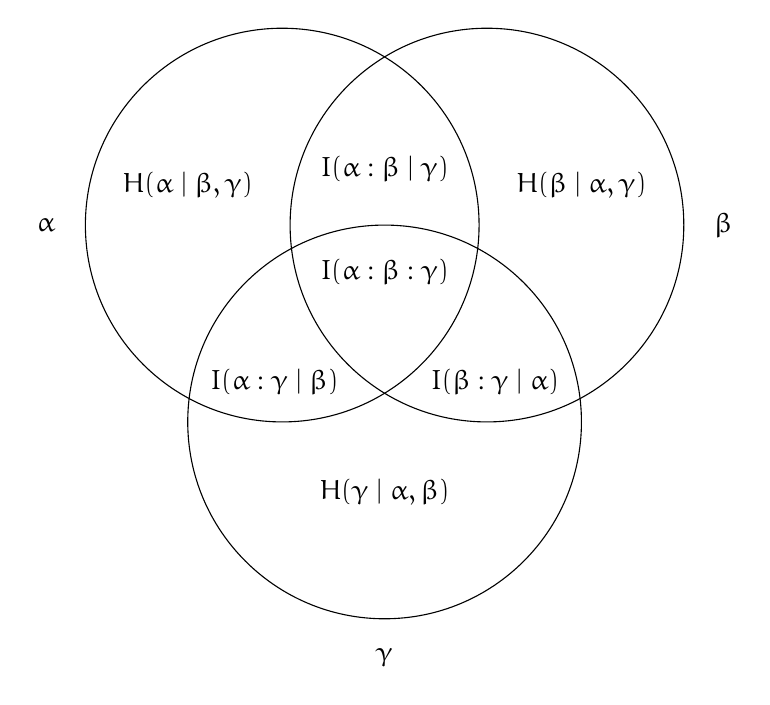
\begin{tikzpicture}
        \tikzstyle{circ}=[circle, draw, inner sep=0pt, minimum width=5cm]

        \draw(1.2,2) circle(2.5cm) node[xshift=-3cm]{$\alpha$};
        \draw(3.8,2) circle(2.5cm) node[xshift=3cm] {$\beta$};
        \draw(2.5,-0.5) circle(2.5cm) node[yshift=-3cm] {$\gamma$};

        \node at (0,2.5) {$H(\alpha \mid \beta, \gamma)$};
        \node at (5,2.5) {$H(\beta \mid \alpha, \gamma)$};
        \node at (2.5,-1.4) {$H(\gamma \mid \alpha, \beta)$};

        \node at (1.1,0) {$I(\alpha : \gamma \mid \beta)$};
        \node at (2.5,2.7) {$I(\alpha : \beta \mid \gamma)$};
        \node at (3.9,0) {$I(\beta : \gamma \mid \alpha)$};

        \node at (2.5,1.4) {$I(\alpha : \beta : \gamma)$};
    \end{tikzpicture}
    \end{center}
We can verify that this results in a correct representation. For example, the area of circle \(\alpha\) will correspond to
\[
H(\alpha) = H(\alpha \mid \beta, \gamma) + I(\alpha : \beta \mid \gamma)
+ I(\alpha : \gamma \mid \beta) + I(\alpha : \beta : \gamma),
\]
and the intersection of circles \(\alpha\) and \(\beta\) will correspond to
\[
I(\alpha : \beta) = I(\alpha : \beta \mid \gamma) + I(\alpha : \beta : \gamma).
\]
In the future, we will use this geometric interpretation to prove relationships involving information quantities.

\begin{statement}
    The total information of three random variables can be negative.
\end{statement}
\begin{proof}
    Let \(\alpha\) and \(\beta\) be independent uniformly distributed random variables over \(\{0, 1\}\). The random variable \(\gamma\) will take a value from \(\{0, 1\}\) according to the following relationship:
    \[
        \alpha \oplus \beta \oplus \gamma = 0.
    \]
    We will obtain the following picture:

    \begin{center}
    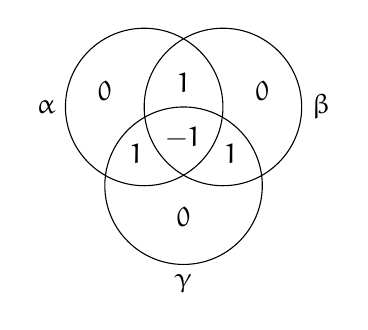
\begin{tikzpicture}
        \tikzstyle{circ}=[circle, draw, inner sep=0pt, minimum width=2cm]

        \node[circ, label=left:$\alpha$]  (a) at (1,1) {};
        \node[circ, label=right:$\beta$]  (b) at (2,1) {};
        \node[circ, label=below:$\gamma$] (c) at (1.5,0) {};
        \node at (0.5,1.2) {$0$};
        \node at (1.5,-.4) {$0$};
        \node at (2.5,1.2) {$0$};

        \node at (0.9,0.4) {$1$};
        \node at (1.5,1.3) {$1$};
        \node at (2.1,0.4) {$1$};

        \node at (1.5,0.6) {$-1$};
    \end{tikzpicture}
    \end{center}
\end{proof}
\begin{statement}
    There are no other inequalities for triples.
\end{statement}
\begin{statement}
    There are profiles that cannot be realized by any distributions, but they have measure 0.
\end{statement}
\begin{exercise}
    Prove that the following profile is realized only when \(h = \log n\) for some integer \(n\).
    \begin{center}
    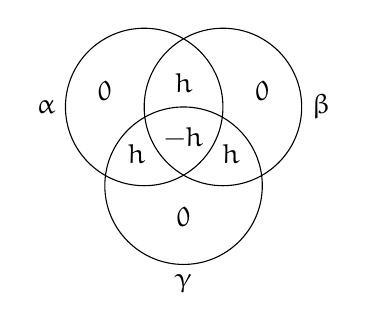
\begin{tikzpicture}
        \tikzstyle{circ}=[circle, draw, inner sep=0pt, minimum width=2cm]

        \node[circ, label=left:$\alpha$]  (a) at (1,1) {};
        \node[circ, label=right:$\beta$]  (b) at (2,1) {};
        \node[circ, label=below:$\gamma$] (c) at (1.5,0) {};
        \node at (0.5,1.2) {$0$};
        \node at (1.5,-.4) {$0$};
        \node at (2.5,1.2) {$0$};

        \node at (0.9,0.4) {$h$};
        \node at (1.5,1.3) {$h$};
        \node at (2.1,0.4) {$h$};

        \node at (1.5,0.6) {$-h$};
    \end{tikzpicture}
    \end{center}
\end{exercise}
\begin{statement}
    \(2H(\alpha, \beta, \gamma) \le H(\alpha, \beta) + H(\alpha, \gamma) + H(\beta, \gamma)\).
\end{statement}
\begin{proof}
    Note how many times each area appears in the left/right part of the inequality.
    \begin{center}
    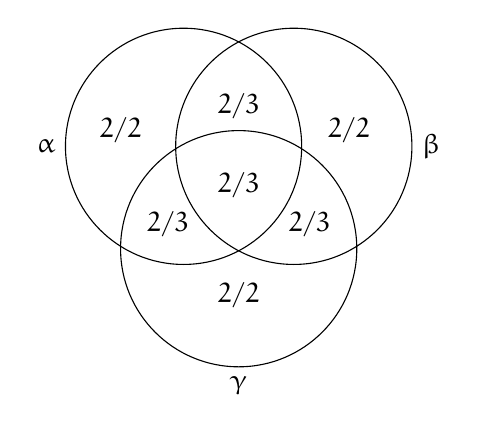
\begin{tikzpicture}
        \tikzstyle{circ}=[circle, draw, inner sep=0pt, minimum width=3cm]

        \node[circ, label=left:$\alpha$]  (a) at (1,1.3) {};
        \node[circ, label=right:$\beta$]  (b) at (2.4,1.3) {};
        \node[circ, label=below:$\gamma$] (c) at (1.7,0) {};
        \node at (0.2,1.5) {$2/2$};
        \node at (3.1,1.5) {$2/2$};
        \node at (1.7,-.6) {$2/2$};

        \node at (0.8,0.3) {$2/3$};
        \node at (2.6,0.3) {$2/3$};
        \node at (1.7,1.8) {$2/3$};

        \node at (1.7,0.8) {$2/3$};
    \end{tikzpicture}
    \end{center}
Thus, the statement simplifies to \(0 \le I(\beta : \gamma) + I(\alpha : \beta \mid \gamma) +
I(\alpha : \gamma \mid \beta)\).
\end{proof}

\begin{corollary}[Theorem~\ref{thm:volume}]
For \(A \subset \bitstr \times \bitstr \times \bitstr\)
\[2\chi(A) \le \chi_{12}(A) + \chi_{13}(A) + \chi_{23}(A).\]
\end{corollary}
\begin{proof}
    Let \((\alpha, \beta, \gamma)\) be uniformly distributed over \(A\) (i.e., the random variables are the coordinates of points in the set \(A\)).
    \[
        2\chi(A) = 2H(\alpha, \beta, \gamma) \le
        \underbrace{H(\alpha, \beta)}_{\le \chi_{12}(A)} +
        \underbrace{H(\alpha, \gamma)}_{\le \chi_{13}(A)} +
        \underbrace{H(\beta, \gamma)}_{\le \chi_{23}(A)}.
    \]
\end{proof}
We can consider a generalization of this theorem for an arbitrary number of coordinates.
\begin{theorem}[Shirer's Lemma]
    Let \(X\) be a random variable distributed over \(\bits^n\).
    For any distribution \(S\) on subsets of \([n]\), where
    \(\Pr[i \in S] \ge \mu\), it holds that \(\E[H(X_S)] \ge \mu \cdot H(X)\).
\end{theorem}
\begin{proof}
    For any set \(T = \{\seqn{i}{k}\} \subset [n]\),
    \(i_1 < i_2 < \dotsb < i_k\), we have
    \[
        H(X_T) = H(X_{i_1}) + H(X_{i_2} \mid X_{i_1}) + \dotsb + H(X_{i_k} \mid X_{i_1}, \dotsc, X_{i_{k-1}}).
    \]
    We will use the fact that \(H(X_{i_t} \mid X_{i_1}, \dotsc, X_{i_{t-1}}) \ge H(X_{i_t} \mid X_{<i_t})\), then
    \[
        H(X_T)
        \ge H(X_{i_1} \mid X_{<i_1}) + H(X_{i_2} \mid X_{<i_2}) + \dotsb + H(X_{i_k} \mid X_{<i_k}).
    \]
    Now let’s apply this fact to the distribution \(S\).
    \begin{align*}
        \E_S[H(X_S)]
        &\ge \E_S\biggl[\sum_{i \in S} H(X_i \mid X_{<i})\biggr]
         = \sum_{i \in [n]} \Pr[i \in S] \cdot H(X_i \mid X_{<i})\\
        &\ge \mu \sum_{i \in [n]} H(X_i \mid X_{<i}) = \mu \cdot H(X).\tag*{\qedhere}
    \end{align*}
\end{proof}
Shirer's Lemma has many applications.
\begin{example}[Counting Triangles in a Graph]
    Let \(G = (V, E)\) be an undirected graph with \(t\) triangles, and let \(\ell = |E|\). We will show that \(t \le \frac{(2\ell)^{3/2}}{6}\).
    \begin{proof}
        Let the triplet of random variables \((\alpha, \beta, \gamma)\) be uniformly distributed over the vertices of the triangles, and let \(X = (\alpha, \beta, \gamma)\). Then \(H(X) = H(\alpha, \beta, \gamma) = \log(6t)\), since each triangle occurs with six different permutations. Consider the distribution \(S\), uniform on subsets \(\{1, 2, 3\}\) of size 2. Then \(\Pr[i \in S] = \frac{2}{3}\). By Shirer's Lemma,
    \[
        \E_S[H(X_S)] \ge \frac{2}{3} \log(6t),
    \]
    i.e., there exists \(T \subset \{1, 2, 3\}\) for which \(H(X_T) \ge \frac{2}{3} \log(6t)\).
    On the other hand, \(X_T\) is a distribution over the edges of the graph, so \(\log(2\ell) \ge H(X_T)\). From this, we get that \(2\ell \ge (6t)^{2/3}\).
    \end{proof}
    A generalization for embedding arbitrary graphs can be found in~\cite{rao10}.
\end{example}

\begin{statement}\label{st:someentropyineq}
    For any \(\alpha\), \(\beta\), and \(\gamma\), the following inequality holds:
    \[
        H(\gamma) \le H(\gamma \mid \alpha) + H(\gamma \mid \beta) + I(\alpha : \beta).
    \]
\end{statement}
If \(H(\gamma \mid \alpha) = H(\gamma \mid \beta) = 0\)
(i.e., \(\gamma\) is uniquely determined by both \(\alpha\) and \(\beta\)),
then \(H(\gamma) \le I(\alpha : \beta)\).
\begin{proof}
    Let’s note how many times each area appears in the left/right part of the inequality.
    \begin{center}
    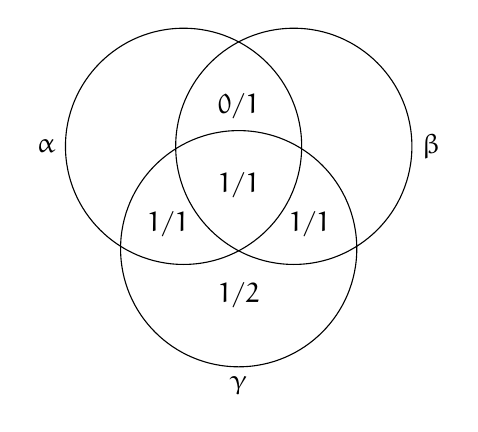
\begin{tikzpicture}
        \tikzstyle{circ}=[circle, draw, inner sep=0pt, minimum width=3cm]

        \node[circ, label=left:$\alpha$]  (a) at (1,1.3) {};
        \node[circ, label=right:$\beta$]  (b) at (2.4,1.3) {};
        \node[circ, label=below:$\gamma$] (c) at (1.7,0) {};
        \node at (1.7,-.6) {$1/2$};
        \node at (1.7,1.8) {$0/1$};
        \node at (1.7,0.8) {$1/1$};

        \node at (0.8,0.3) {$1/1$};
        \node at (2.6,0.3) {$1/1$};

    \end{tikzpicture}
    \end{center}
    Thus, the inequality simplifies to \(0 \le H(\gamma \mid \alpha, \beta) +
    I(\alpha : \beta \mid \gamma)\).
\end{proof}
\begin{exercise}
    Suppose \(\alpha \to \beta \to \gamma\) forms a Markov chain, i.e., the distribution
    \(\langle \gamma \mid \beta \rangle = \langle \gamma \mid \alpha, \beta \rangle\).
    Prove that \(I(\alpha : \gamma) \le I(\alpha : \beta)\) and \(I(\alpha : \gamma) \le I(\beta : \gamma)\).
\end{exercise}
\begin{exercise}
    Suppose \(\alpha \to \beta \to \gamma \to \delta\) forms a Markov chain.
    Prove that \(I(\alpha : \beta) \le I(\beta : \gamma)\).
\end{exercise}
\begin{exercise}\label{ex:existsdelta}
    Let \(\alpha\), \(\beta\), and \(\gamma\) have the following profile.
    \begin{center}
    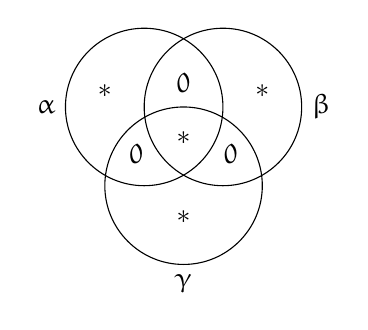
\begin{tikzpicture}
        \tikzstyle{circ}=[circle, draw, inner sep=0pt, minimum width=2cm]

        \node[circ, label=left:$\alpha$]  (a) at (1,1) {};
        \node[circ, label=right:$\beta$]  (b) at (2,1) {};
        \node[circ, label=below:$\gamma$] (c) at (1.5,0) {};
        \node at (0.5,1.2) {$*$};
        \node at (1.5,-.4) {$*$};
        \node at (2.5,1.2) {$*$};

        \node at (0.9,0.4) {$0$};
        \node at (1.5,1.3) {$0$};
        \node at (2.1,0.4) {$0$};

        \node at (1.5,0.6) {$*$};
    \end{tikzpicture}
    \end{center}
    Prove that there exists a random variable \(\delta\) such that
    \[
        \begin{cases}
            H(\delta \mid \alpha) = 0,\\
            H(\delta \mid \beta)  = 0,\\
            H(\delta \mid \gamma) = 0,\\
            H(\delta) = I(\alpha : \beta : \gamma).
        \end{cases}
    \]
    Moreover, \(I(\alpha : \beta \mid \delta) = I(\alpha : \gamma \mid \delta) = I(\beta : \gamma \mid \delta) = 0\).
\end{exercise}
\begin{exercise}
    Let’s take random variables from the previous exercise as \(x, y, a, b\): \(x = \alpha\),
    \(y = \beta\), \(a = \gamma\), \(b = \delta\). Show that for any such \((a, b, x, y)\) from the condition
    \(I(x : y \mid a) = I(x : a \mid y) = I(y : a \mid x) = 0\), it follows that
    \[
        I(a : b) \le I(a : b \mid x) + I(a : b \mid y) + I(x : y).
    \]
    [Hint: Apply the inequality from statement~\ref{st:someentropyineq}.]
\end{exercise}
\begin{exercise}
    Let’s take random variables from exercise~\ref{ex:existsdelta} as \(x, y, a, b\): \(x = \alpha\),
    \(y = \beta\), \(a = \gamma\), \(b = \delta\). Show that there exist such \((a, b, x, y)\) for which
    \[
        I(a : b) \not\le I(a : b \mid x) + I(a : b \mid y) + I(x : y).
    \]
    (That is, the condition in the previous exercise was necessary.)
\end{exercise}
\begin{statement}[Inequality for 5 Random Variables]
    \[
        I(a : b) \le I(a : b \mid x) + I(a : b \mid y) + I(x : y)
        + I(a : b \mid z) + I(a : z \mid b) + I(b : z \mid a).
    \]
\end{statement}
\begin{corollary}[Zhang, Yeung, 1998]
    An inequality for 4 random variables that cannot be expressed through the basic inequalities.
    \[
        I(a : b) \le 2I(a : b \mid x) + I(a : b \mid y) + I(x : y)
        + I(a : x \mid b) + I(b : x \mid a).
    \]
\end{corollary}
\begin{statement}
    For 4 random variables, there are infinitely many inequalities that are independent of each other.
\end{statement}

\subsection{Inequalities for Triplets}
We will prove the following statement under various assumptions:
\[
    H(a \mid x) + H(a \mid y) \le H(a).
\]

\begin{statement}
    If \(a, x, y\) are such that
\[
    \begin{cases}
        H(a \mid x, y) = 0,\\
        I(x : y \mid a) = 0.
    \end{cases}
\]
then \(H(a \mid x) + H(a \mid y) \le H(a)\).
\end{statement}
\begin{proof}
    We need to prove the non-negativity of \(h\).
    \begin{center}
    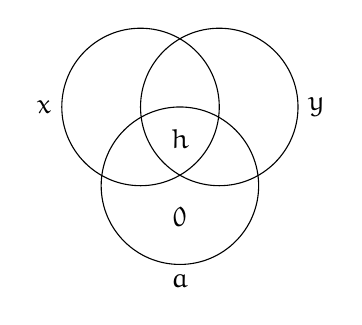
\begin{tikzpicture}
        \tikzstyle{circ}=[circle, draw, inner sep=0pt, minimum width=2cm]

        \node[circ, label=left:$x$]  (x) at (1,1) {};
        \node[circ, label=right:$y$] (y) at (2,1) {};
        \node[circ, label=below:$a$] (a) at (1.5,0) {};
        \node at (1.5,-.4) {$0$};

        \node at (1.5,0.6) {$h$};
    \end{tikzpicture}
    \end{center}
Since \(I(x : y \mid a) = 0\), it follows that \(h = I(x : y) \ge 0\).
\end{proof}
\begin{statement}\label{st:entropy:triple-rect}
    If \(a, x, y\) are such that \(H(a \mid x, y) = 0\) and
\[
    \begin{cases}
        A_i \sim X_j\\
        A_i \sim Y_k
    \end{cases} \implies A_i \sim (X_j, Y_k),
\]
then \(H(a \mid x) + H(a \mid y) \le H(a)\). (The notation \(A_i \sim X_j\) means \(\Pr[a = A_i \land x = X_j] > 0\).)
\end{statement}
\begin{remark}
    The condition \(H(a \mid x, y) = 0\) can be interpreted as \(a = f(x, y)\).
\end{remark}
% todo: ask Shenya how to explain this more simply
\begin{proof}
    We will construct a new distribution \((a', x', y')\):
    \begin{itemize}
        \item \(a'\) has the same distribution as \(a\),
        \item the conditional distribution of \(x'\) given \(a'\) coincides
            with the conditional distribution of \(x\) given \(a\),
        \item the conditional distribution of \(y'\) given \(a'\) coincides
            with the conditional distribution of \(y\) given \(a\),
        \item \(x'\) and \(y'\) are independent.
    \end{itemize}
    \[
    \Pr[a' = A_i, x' = X_j, y' = Y_k] =
    \Pr[a' = A_i] \cdot \Pr[x' = X_j \mid a' = A_i] \cdot \Pr[y' = Y_k \mid a' = A_i].
    \]
    Thus,
    \[
        H(a', x', y') = H(a') + H(x' \mid a') + H(y' \mid a') - \underbrace{I(x' : y' \mid a')}_{0}.
    \]
    On the other hand,
    \[
        H(a', x', y') \le H(x') + H(y') + H(a' \mid x', y').
    \]
    Furthermore, we can erase the indicators almost everywhere.
    \[
        H(x) + H(y) + H(a' \mid x', y') \ge H(a', x', y') = H(a) + H(x \mid a) + H(y \mid a).
    \]
    We will show that \(H(a' \mid x', y') = 0\), i.e., \(a' = f(x', y')\). Indeed:
    if the triplet \((A_i, X_j, Y_k)\) in the new distribution appears with positive
    probability, then it also appeared in the original distribution with positive
    probability, hence \(a' = f(x', y')\).
    We get: \(H(a) + H(x \mid a) + H(y \mid a) \le H(x) + H(y)\). Adding \(H(a)\) to both sides of the inequality:
    \[
       H(x, a) + H(y, a) \le H(x) + H(y) + H(a) \implies H(a \mid x) + H(a \mid y) \le H(a). \qedhere
    \]
\end{proof}
\begin{problem}[Vereshchagin~\cite{KRV18}]
    Consider a bipartite graph with vertices \((L, R)\) with colored edges.
    All edges incident to a single vertex are of different colors, the degree in the left part is at least \(n\),
    and in the right part is at least \(m\). Suppose it is known that for a pair of vertices \((x \in L, y \in R)\)
    there is at most one common color. Prove that the number of colors is at least \(n \cdot m\).

    Note that monochrome edges form matchings. For each color \(c\), connect all
    vertices on the left that are matched with \(c\) to those on the right that are matched with \(c\). This forms a biclique of
    edges of color \(c\).

    Consider the distribution on triplets \((a, x, y)\) (color, vertex from the left part, vertex from the right
    part): we choose the color proportionally to the size (number of edges) of the corresponding biclique and
    select a random edge of that color. It can be checked that the following relation holds:
\[
    \begin{cases}
        A_i \sim X_j,\\
        A_i \sim Y_k,
    \end{cases} \implies A_i \sim (X_j, Y_k).
\]
Now we apply: \(\underbrace{H(a \mid x)}_{\ge \log n} +
                  \underbrace{H(a \mid y)}_{\ge \log m} \le H(a) \le \log (\text{\# colors})\).
\end{problem}
\subsection{Conditional Inequality for a Quadruple}
\begin{statement}
    If for random variables \(a, b, x, y\) the following holds
    \[
        \begin{cases}
            I(x:y \mid a) = 0,\\
            H(a \mid x, y) = 0,
        \end{cases}
    \]
    then \(I(a:b) \le I(a:b \mid x) + I(a:b \mid y) + I(x:y)\).
\end{statement}
\begin{proof}
    We will construct a new distribution \((a', b', x', y')\):
    first, we choose a value \((a', b') \sim (a, b)\).
    For a fixed value of \((a', b')\), we independently choose \(x'\) and \(y'\) such that the conditional probability distributions with respect to \(a'\) are the same as those of \(x\) and \(y\) with respect to \(a\).
    \begin{multline*}
    H(a', b', x', y') = H(a', b') + H(x \mid a', b') + H(y \mid a', b') - \underbrace{I(x':y' \mid a', b')}_{0} =\\
    = H(a, b) + H(x \mid a, b) + H(y \mid a, b).
    \end{multline*}
    On the other hand,
    \begin{multline*}
    H(a', b', x', y') \le H(b') + H(x' \mid b') + H(y' \mid b') + H(a' \mid x', y') =\\
    = H(b) + H(x \mid b) + H(y \mid b) + H(a' \mid x', y').
    \end{multline*}
    We will show that \(H(a' \mid x', y') = 0\). This was satisfied in the original distribution by assumption.
    Let \([a' = A_i, x' = X_j, y' = Y_k]\) in the new distribution occur with positive probability. Therefore, it also occurs in the original distribution with positive probability (given a fixed \(a'\), \(x'\) and \(y'\) are independent), which preserves the corresponding functional dependence of \(a'\) on \((x', y')\).

    As a result, we obtain
    \[
        H(a, b) + H(x \mid a, b) + H(y \mid a, b) \le H(b) + H(x \mid b) + H(y \mid b).
    \]
    We can rewrite this inequality using unconditional entropies:
    \[
        H(a, b) + H(x, a, b) - H(a, b) + H(y, a, b) - H(a, b) \le H(b) + H(x, b) - H(b) + H(y, b) - H(b).
    \]
    Simplifying gives us:
    \begin{equation}\label{eq:condineq1}
        H(x, a, b) + H(y, a, b) + H(b) \le H(x, b) + H(y, b) + H(a, b).
    \end{equation}
    Now we will do the same for \(I(a:b) \le I(a:b \mid x) + I(a:b \mid y) + I(x:y)\).
    \begin{equation*}
        \begin{array}{ll}
        H(a) + H(b) - H(a, b) \le
        & H(a, x) + H(b, x) - H(a, b, x) - H(x) + \mbox{} \\
        & H(a, y) + H(b, y) - H(a, b, y) - H(y) + \mbox{} \\
        & H(x) + H(y) - H(x, y).
        \end{array}
    \end{equation*}
    Simplifying yields:
    \begin{equation}\label{eq:condineq2}
        \begin{array}{ll}
        H(a, b, x) + H(a, b, y) + H(b) + H(x, y) \le
        & H(b, x) + H(b, y) + H(a, b) + \mbox{} \\
        & H(a, x) + H(a, y) - H(a).
        \end{array}
    \end{equation}

    Note that we only need to prove \(H(x, y) \le H(a) + H(x \mid a) + H(y \mid a)\).
    Adding this inequality to \eqref{eq:condineq1} will yield \eqref{eq:condineq2}.
    Let’s note how many times each area contributes to the left/right side of the inequality.
    \begin{center}
    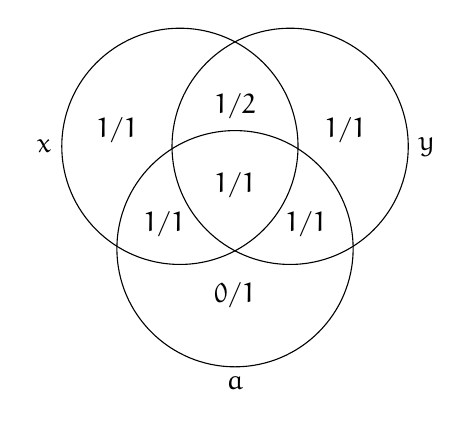
\begin{tikzpicture}
        \tikzstyle{circ}=[circle, draw, inner sep=0pt, minimum width=3cm]

        \node[circ, label=left:$x$]  (a) at (1,1.3) {};
        \node[circ, label=right:$y$] (b) at (2.4,1.3) {};
        \node[circ, label=below:$a$] (c) at (1.7,0) {};
        \node at (0.2,1.5) {$1/1$};
        \node at (3.1,1.5) {$1/1$};
        \node at (1.7,-.6) {$0/1$};

        \node at (0.8,0.3) {$1/1$};
        \node at (2.6,0.3) {$1/1$};
        \node at (1.7,1.8) {$1/2$};

        \node at (1.7,0.8) {$1/1$};
    \end{tikzpicture}
    \end{center}
    That is, it is equivalent to \(H(a \mid x, y) + I(x:y \mid a) \ge 0\).
\end{proof}
Questions to think about: Come up with an interpretation for this inequality. Zhang and Yeung proved this same inequality in 1997 under the assumption \(I(x:y) = I(x:y \mid a) = 0\). Is there a combinatorial interpretation of this statement?

\begin{exercise}
A rectangular table is divided into (combinatorial) rectangles such that each row intersects at least \(n\) rectangles and each column intersects at least \(m\) rectangles. Prove that the total number of rectangles is at least \(nm\).
\end{exercise}


\section{Cryptography}
\subsection{Symmetric Key Encryption}

Consider the task of encoding a message using symmetric encryption. We will assume that the computational resources of the adversary are unlimited. Let us suppose that we encrypt a message $m$ with an encryption key $k$. During the encryption of the message, we obtain the \emph{ciphertext} $c = E(k, m)$. The recipient of the ciphertext also knows the key $k$ and can recover the original message $m = D(k, c)$.

We will assume that $m$ and $k$ are random variables. The adversary does not know $m$ and $k$, but knows $c$. For a \emph{perfect} encryption scheme, the following conditions must hold:
\[
\begin{cases}
    H(c \mid k, m) = 0,\\
    H(m \mid k, c) = 0,\\
    I(c : m) = 0.
\end{cases}
\]

\begin{theorem}[Shannon]
    $H(k) \ge H(m)$, even if the condition $H(c \mid k, m) = 0$ is violated
    (i.e., the algorithm $E$ uses random bits).
\end{theorem}
\begin{remark}
    A one-time pad has this property.
\end{remark}
\begin{proof}
    According to the condition, $x + w = 0$, i.e., $x = -w$.

    \begin{center}
        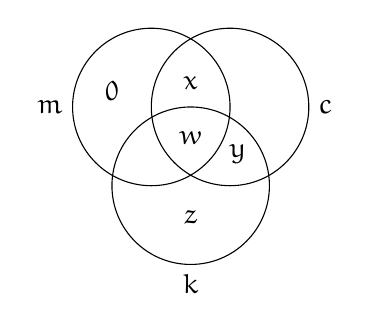
\begin{tikzpicture}
            \tikzstyle{circ}=[circle, draw, inner sep=0pt, minimum width=2cm]

            \node[circ, label=left:$m$]  (x) at (1,1) {};
            \node[circ, label=right:$c$] (y) at (2,1) {};
            \node[circ, label=below:$k$] (z) at (1.5,0) {};
            \node at (0.5,1.2) {$0$};
            \node at (1.5,-.4) {$z$};

            \node at (1.5,1.3) {$x$};
            \node at (2.1,0.4) {$y$};

            \node at (1.5,0.6) {$w$};
        \end{tikzpicture}
    \end{center}
    Since the mutual information is non-negative, we have $w + y \ge 0$, i.e.,
    $y \ge -w = x$. Now, from $y \ge x$ and $z \ge 0$, it follows that $H(k) \ge H(m)$.
\end{proof}

\subsection{Secret Sharing Schemes}

Let us have a certain secret $S_0$ and $n$ participants, and we want to share this secret among them in such a way that they can only use it together, while any subset of participants cannot.

\begin{definition}
    A \emph{perfect secret sharing scheme} is a joint distribution of probabilities $(S_0, \seqn{S}{n})$ such that
    \[
    \begin{cases}
        H(S_0 \mid \seqn{S}{n}) = 0,\\
        H(S_0 \mid \seqin{S}{i}{k}) = H(S_0), & k < n.
    \end{cases}
    \]
    The second condition can be rewritten as $I(S_0 : \seqin{S}{i}{k}) = 0$.
\end{definition}

For a perfect secret sharing scheme, there is a simple construction. Let us assume that $S_0$ is written (encoded) using $\ell$ bits. We will independently and uniformly choose $S_1, \dotsc, S_{n-1} \in \{0,1\}^\ell$. $S_n$ is determined by the condition
$S_0 \oplus S_1 \oplus S_2 \oplus \dotsb \oplus S_n = \vec 0$ (coordinate-wise sum modulo 2).

\begin{statement}
    The proposed secret sharing scheme is perfect.
\end{statement}

\begin{definition}
    A \emph{threshold perfect secret sharing scheme} is a joint distribution of probabilities $(S_0, \seqn{S}{n})$ such that
    \[
    \begin{cases}
        H(S_0 \mid \seqin{S}{i}{t}) = 0,\\
        H(S_0 \mid \seqin{S}{i}{k}) = H(S_0), & k < t.
    \end{cases}
    \]
\end{definition}

\paragraph{Shamir's Threshold Scheme.} Let us assume that the secret $S_0$ is an element of some finite field $\mathbb{F}_q$. We will choose a random polynomial $p$ over the field $\mathbb{F}_q$ of degree at most $t-1$: we will choose $t-1$ coefficients independently and uniformly, and determine the last (constant) coefficient from the condition $p(0) = S_0$. We will randomly select and inform all participants of some set of distinct non-zero elements of the field $\seqn{a}{n} \in \mathbb{F}_q$ and compute the participants' secrets as the value of the polynomial at the corresponding points $S_i = p(a_i)$. Now, any $t$ participants can gather, use the formula for polynomial interpolation, and compute $S_0 = p(0)$. If fewer participants gather, they will have no information about $S_0$.

\begin{statement}
    Shamir's threshold scheme is perfect.
\end{statement}
\begin{proof}
    Any polynomial of degree less than $t-1$ can be extended to a polynomial of higher degree with any value at point $0$.
\end{proof}

\begin{definition}
    A \emph{perfect secret sharing scheme for an access structure $\Gamma \subset 2^{[n]}$} (with $\Gamma$ being upward closed) is a joint distribution of probabilities $(S_0, \seqn{S}{n})$ such that
    \[
    \begin{cases}
        H(S_0 \mid \seqin{S}{i}{m}) = 0, & \{\seqn{i}{m}\} \in \Gamma,\\
        H(S_0 \mid \seqin{S}{i}{m}) = H(S_0), & \{\seqn{i}{m}\} \not\in \Gamma.
    \end{cases}
    \]
\end{definition}

\begin{definition}
    An \emph{ideal secret sharing scheme} is a perfect secret sharing scheme with the additional requirement of "efficiency".
    \[
    \forall i \in \{1, 2, \dotsc, n\},\ H(S_i) \le H(S_0).
    \]
\end{definition}

\begin{statement}
    If participant $i$ is \emph{essential} in the access structure $\Gamma$ (i.e., there exists
    some $s \in \Gamma$ such that $s \setminus \{i\} \not\in \Gamma$), then $H(S_i) \ge H(S_0)$.
\end{statement}

\begin{remark}
    Shamir's scheme is ideal.
\end{remark}

\begin{proof}
    Let $s=\{i, \seqn{j}{k}\} \in \Gamma$, and $s \setminus \{i\} \not\in \Gamma$.
    We denote the mutual information $I(S_0 : \seqin{S}{j}{k} \mid S_i)$ as $h$,
    and $I(S_i : \seqin{S}{j}{k} \mid S_0)$ as $g$. From the condition
    $I(S_0 : \seqin{S}{j}{k}) = 0$, we obtain that
    $I(S_0 : S_i : \seqin{S}{j}{k}) = -h$, and similarly, from
    $I(S_i : \seqin{S}{j}{k}) \ge 0$, we get that $g \ge h$.

    \begin{center}
        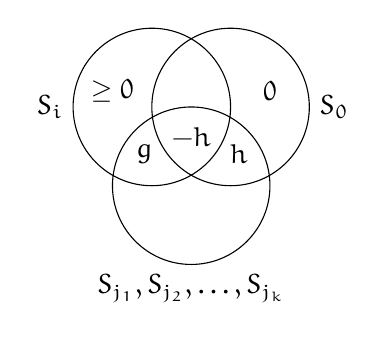
\begin{tikzpicture}
            \tikzstyle{circ}=[circle, draw, inner sep=0pt, minimum width=2cm]

            \node[circ, label=left:$S_i$]  (a) at (1,1) {};
            \node[circ, label=right:$S_0$]  (b) at (2,1) {};
            \node[circ, label=below:$\seqin{S}{j}{k}$] (c) at (1.5,0) {};
            \node at (0.5,1.2) {$\ge 0$};
            \node at (2.5,1.2) {$0$};

            \node at (2.1,0.4) {$h$};
            \node at (0.9,0.4) {$g$};

            \node at (1.5,0.6) {$-h$};
        \end{tikzpicture}
    \end{center}
    Thus, $H(S_i) \ge H(S_0)$.
\end{proof}

\begin{remark}
    This statement shows that there cannot be a more "efficient" secret sharing scheme than an ideal one.
\end{remark}

\begin{statement}
    For any access structure $\Gamma$, there exists a perfect secret sharing scheme.
\end{statement}

\begin{proof}
    Let us create a separate set of secrets $S^A_{i_1}, S^A_{i_2}, \dotsc, S^A_{i_k}$ for each subset
    $A = \{\seqn{i}{k}\} \in \Gamma$: $S^A_{i_1} \oplus S^A_{i_2} \oplus \dotsb \oplus S^A_{i_k} = S_0$.
    (It is sufficient to consider only minimal sets $A$.)
\end{proof}

\begin{remark}
    The proposed scheme is not ideal.
\end{remark}

\begin{statement}
    There exist access structures for which there is no ideal secret sharing scheme.
\end{statement}

\begin{proof}
    Consider the access structure defined by the following graph (the edges correspond to the authorized
    sets).
    \begin{center}
        \begin{tikzpicture}
            \tikzstyle{vert}=[circle, draw, fill=black!50,
            inner sep=0pt, minimum width=4pt]
            \node at (0,0.5) {};
            \foreach \i/\n in {1/a, 2/b, 3/c, 4/d}
            \node[vert, label=below:\i] (\n) at (\i,0) {};

            \path (a) edge (b);
            \path (b) edge (c);
            \path (c) edge (d);
        \end{tikzpicture}
    \end{center}
    We will show that for this access structure, $H(S_2) + H(S_3) \ge 3H(S_0)$, in other words,
    $\max_i \frac{H(S_i)}{H(S_0)} \ge \frac{3}{2}$.

    For the proof, we will need three lemmas. Let us denote $h = H(S_0)$.

    \begin{lemma}
        $H(S_2 \mid S_1, S_3) \ge h$.
    \end{lemma}

    \begin{proof}
        The second participant can recover the secret using either the secret of the first or the secret of the third participant,
        i.e., $I(S_2 : S_0 \mid S_1, S_3) = h$.
        \begin{center}
            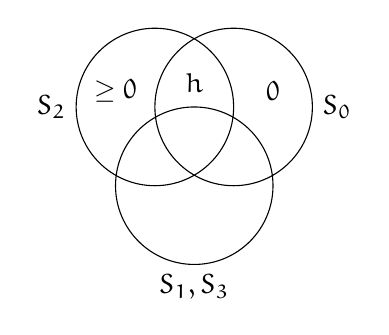
\begin{tikzpicture}
                \tikzstyle{circ}=[circle, draw, inner sep=0pt, minimum width=2cm]

                \node[circ, label=left:$S_2$]  (a) at (1,1) {};
                \node[circ, label=right:$S_0$]  (b) at (2,1) {};
                \node[circ, label=below:{$S_1, S_3$}] (c) at (1.5,0) {};
                \node at (0.5,1.2) {$\ge 0$};
                \node at (2.5,1.2) {$0$};
                \node at (1.5,1.3) {$h$};
            \end{tikzpicture}
        \end{center}
        Thus, $H(S_2 \mid S_1, S_3) \ge I(S_2 : S_0 \mid S_1, S_3) = h$.
    \end{proof}

    \begin{lemma}
        $H(S_3 \mid S_1) \ge h$.
    \end{lemma}

    \begin{proof}
        Similarly to the previous lemma, we obtain that $H(S_3 \mid S_1, S_4) \ge h$, and consequently,
        $H(S_3 \mid S_1) \ge h$.
        \begin{center}
            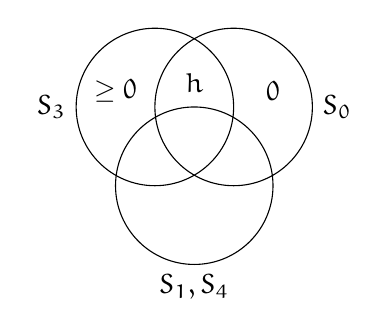
\begin{tikzpicture}
                \tikzstyle{circ}=[circle, draw, inner sep=0pt, minimum width=2cm]

                \node[circ, label=left:$S_3$]  (a) at (1,1) {};
                \node[circ, label=right:$S_0$]  (b) at (2,1) {};
                \node[circ, label=below:{$S_1, S_4$}] (c) at (1.5,0) {};
                \node at (0.5,1.2) {$\ge 0$};
                \node at (2.5,1.2) {$0$};
                \node at (1.5,1.3) {$h$};
            \end{tikzpicture}
        \end{center}
    \end{proof}

    \begin{lemma}\label{lm:secret4:l3}
        $I(S_1 : S_3 \mid S_2) \ge h$.
    \end{lemma}

    \begin{proof}
        The following scheme should be interpreted as entropy conditioned on $S_2$.
        \begin{center}
            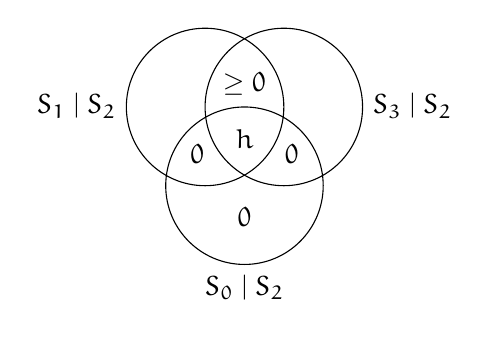
\begin{tikzpicture}
                \tikzstyle{circ}=[circle, draw, inner sep=0pt, minimum width=2cm]

                \node[circ, label=left: $S_1 \mid S_2$]  (a) at (1,1) {};
                \node[circ, label=right:$S_3 \mid S_2$]  (b) at (2,1) {};
                \node[circ, label=below:$S_0 \mid S_2$] (c) at (1.5,0) {};

                \node at (0.9,0.4) {$0$};
                \node at (1.5,1.3) {$\ge 0$};
                \node at (2.1,0.4) {$0$};

                \node at (1.5,-.4) {$0$};
                \node at (1.5,0.6) {$h$};
            \end{tikzpicture}
        \end{center}
        Note that $I(S_1 : S_0 \mid S_2) = h$ and $I(S_3 : S_0 \mid S_2) = h$, while
        $I(S_1 : S_0 \mid S_2, S_3) = 0$ and $I(S_3 : S_0 \mid S_1, S_2) = 0$.
        Thus, $I(S_1 : S_3 : S_0 \mid S_2) = h$, hence $I(S_1 : S_3 \mid S_2) \ge h$.
    \end{proof}

    Now we just need to sum the results of the three lemmas:
    \[
    H(S_2) + H(S_3) \ge H(S_2, S_3) = H(S_2 \mid S_1, S_3) + H(S_3 \mid S_1) + I(S_1 : S_3 \mid S_2) +
    I(S_2 : S_1) \ge 3h.
    \]
\end{proof}

\begin{exercise}
    Prove that for any secret sharing scheme for this structure,
    $\max_i \frac{H(S_i)}{H(S_0)} \ge \frac{3}{2}$.
    \begin{center}
        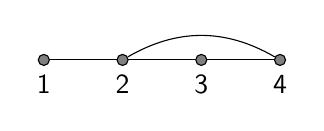
\begin{tikzpicture}
            \tikzstyle{vert}=[circle, draw, fill=black!50,
            inner sep=0pt, minimum width=4pt]
            \node[vert, label=below:1] (a) at (1,0) {};
            \node[vert, label=below:4] (d) at (4,0) {};

            \path (a) edge (d);

            \node[vert, label=below:2] (b) at (2,0) {};
            \node[vert, label=below:3] (c) at (3,0) {};

            \path (b) edge[bend left] (d);
        \end{tikzpicture}
    \end{center}
\end{exercise}

\begin{theorem}[Csirmaz'94]
    There exist access structures $\Gamma$ on $n$ participants such that for any secret sharing scheme,
    $\max_i \frac{H(S_i)}{H(S_0)} \ge \Omega\left(\frac{n}{\log n}\right)$.
\end{theorem}

\begin{proof}
    Choose $n$ and $k$ such that $n = 2^k + k - 1$, and two sets of participants
    \[
    \begin{array}{l}
        A = \{\seqn{a}{k}\},\\
        B = \{\seqn{b}{2^k - 1}\}.
    \end{array}
    \]
    To define the access structure, we need two families of sets. Let $\{A_0, \seqn{A}{2^k-1}\}$ be all subsets of $A$, where $A_0 = A$ and for any $i < j$, $A_i \not\subseteq A_j$ (for example, they can be ordered by decreasing size). We will construct the sets $\{B_0, \seqn{B}{2^k - 1}\}$ as follows: $B_0 = \emptyset$, $B_i = \{\seqn{b}{i}\}$. Now we are ready to define the access structure $\Gamma$: $\Gamma = \{U_i\}_{i=0}^{2^k-1}$, where $U_i = A_i \cup B_i$.

    As in previous statements, we denote $H(S_0)$ as $h$. In the following reasoning, we will use the following notation: by the entropy of a set of participants $X = \{\seqn{x}{t}\} \subset A \cup B$, we will mean the entropy of the secrets belonging to the participants of this set, i.e., $H(X) = H(\seqin{S}{x}{t})$.

    \begin{lemma}\label{lm:secretlb}
        For $i = \{0, 1, 2, \dots, 2^k-2\}$
        \[
        H(A \cup B_i) - H(B_i) \ge H(A \cup B_{i+1}) - H(B_{i+1}) + h.
        \]
    \end{lemma}

    From this lemma, it follows that
    \begin{multline*}
        H(A) = H(A \cup B_0) - H(B_0) \ge H(A \cup B_{1}) - H(B_1) + h \ge \dotsb \ge\\
        \ge \underbrace{H(A \cup B_{2^k-1}) - H(B_{2^k-1})}_{\ge 0} + (2^k - 1) \cdot h.
    \end{multline*}
    Thus, we obtain that $H(A) = H(\seqin{S}{a}{k}) \ge (2^k - 1) \cdot h$. Consequently, there exists an $i$ such that $H(S_{a_i}) \ge \frac{2^k - 1}{k} \cdot h$.
    Recall that we chose $n = 2^k + k - 1$, i.e., $H(S_{a_i}) \ge \Omega\left(\frac{n}{\log n}\right) \cdot h$. It remains to prove the lemma.

    \begin{proof}[Proof of lemma~\ref{lm:secretlb}]
        We will prove two inequalities:
        \begin{enumerate}
            \item $H(A_{i+1} \cup B_i) + H(B_{i+1}) \ge H(A_{i+1} \cup B_{i+1}) + H(B_i)$.
            \item $H(A \cup B_i) + H(A_{i+1} \cup B_{i+1}) \ge H(A \cup B_{i+1}) + H(A_{i+1} \cup B_i) + h$.
        \end{enumerate}
        Note that if we add these two inequalities, we will obtain the statement of the lemma.

        The first inequality states the non-negativity of conditional joint information.
        Indeed, let us recall the formula for conditional joint information:
        \[
        I(x:y \mid z) \ge 0 \iff H(x,z) + H(y,z) \ge H(x,y,z) + H(z).
        \]
        Thus, the first inequality asserts that $I(A_{i+1} : \{b_{i+1}\} \mid B_i) \ge 0$.

        Similarly, the second inequality asserts that $I(A : \{b_{i+1}\} \mid A_{i+1} \cup B_i) \ge h$.
        The proof of this assertion is analogous to lemma~\ref{lm:secret4:l3}—it is necessary to consider the conditional distribution given $A_{i+1} \cup B_i$.
        \begin{center}
            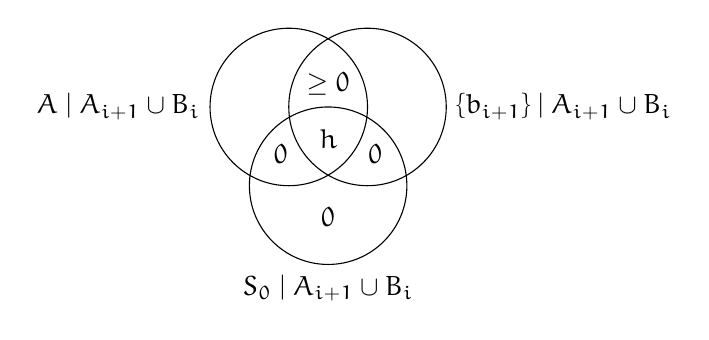
\begin{tikzpicture}
                \tikzstyle{circ}=[circle, draw, inner sep=0pt, minimum width=2cm]

                \node[circ, label=left:$A \mid A_{i+1} \cup B_i$]  (a) at (1,1) {};
                \node[circ, label=right:{$\{b_{i+1}\} \mid A_{i+1} \cup B_i$}]  (b) at (2,1) {};
                \node[circ, label=below:{$S_0 \mid A_{i+1} \cup B_i$}] (c) at (1.5,0) {};
                \node at (0.9,0.4) {$0$};
                \node at (1.5,1.3) {$\ge 0$};
                \node at (2.1,0.4) {$0$};

                \node at (1.5,-.4) {$0$};
                \node at (1.5,0.6) {$h$};
            \end{tikzpicture}
        \end{center}
    \end{proof}
    This lemma concludes the proof of the theorem.
\end{proof}

\begin{remark}
    Lower bounds on the excessive complexity of perfect secret sharing schemes imply lower bounds on the circuit complexity of monotonic functions.
\end{remark}



\section{Communication Complexity}
Let $X$, $Y$, and $Z$ be three finite sets, and let a function $f: X \times Y \to Z$ be given. Two players, whom we will call Alice and Bob, solve the \emph{communication problem for the function $f$} if:
\begin{enumerate}
    \item The sets $X$, $Y$, $Z$, and the function $f$ are known to both players,
    \item Alice knows some $x \in X$,
    \item Bob knows some $y \in Y$,
    \item Alice and Bob aim to compute $f(x,y)$.
\end{enumerate}
To solve this communication problem, Alice and Bob can send messages to each other. The task is considered solved if both players know $f(x,y)$. We are interested in the minimum number of bits that need to be sent to compute $f(x,y)$.

\begin{definition}
    A \emph{communication protocol} for the function $f: X \times Y \to Z$ is a rooted binary tree that describes the joint computation of the function $f$ by Alice and Bob. In this tree, each internal vertex $v$ is labeled with either A or B, indicating whose turn it is, Alice's or Bob's, respectively. For each vertex labeled A, a function $g_v: X \to \bits$ is defined, which tells Alice which bit to send if the computation is at this vertex. Similarly, for each vertex $v$ labeled B, a function $h_v: Y \to \bits$ is defined, which specifies the bit that Bob should send at this vertex. Each internal vertex has two children, with the edge to the first child labeled $0$, and the edge to the second child labeled $1$. Each leaf is labeled with a value from the set $Z$.

    The computation according to such a protocol on a specific pair of inputs $(x,y)$ is structured as follows: initially, the computation is at the root. At each internal vertex $v$, depending on the label, either Alice or Bob sends one bit (determined by the corresponding function $g_v$ or $h_v$). After this, the computation moves to one of the children of vertex $v$ through the edge labeled with the bit sent at vertex $v$. When the computation reaches a leaf, it concludes. The result of the computation is the label at the leaf.
\end{definition}

We will say that the communication protocol \emph{computes the function $f$} if for all pairs $(x,y) \in X \times Y$, the computation reaches a leaf labeled $f(x,y)$. We can now give a formal definition of the \emph{communication complexity of the function $f$}.

Analogously, we can define a \emph{communication protocol that computes the relation $R \subset (X \times Y) \times Z$}—we just need to additionally require that Alice's and Bob's responses are consistent.

\begin{definition}
    The \emph{communication complexity} of the function $f$ is defined as the smallest depth of the protocol (the maximum edge length of the path from the root to a leaf) that computes the function $f$. It is denoted as $D(f)$.
\end{definition}

\begin{statement}
    For any $f: \{0,1\}^n \times\{0,1\}^n \to \bits$, $D(f) \le n + 1$.
\end{statement}
\begin{proof}
    Alice sends her input to Bob, and Bob sends Alice the value of $f$.
\end{proof}

\begin{example} Examples of functions with non-trivial upper bounds on communication complexity.
    \begin{enumerate}
        \item (Pointer Chasing) $D(\mathrm{PC}) \le k \log n$,
        where \[PC(x,y) = \underbrace{x(y(x(y(x(y(x(y(x}_{\text{$k$ rounds}}(0))))))))).\]
        The players have a bipartite directed graph with $2n$ vertices, where the out-degree of each vertex is 1. Alice knows the left part, and Bob knows the right part. Initially, they place a token on vertex 0 from Alice's part and start moving it along the edges. They need to make $k$ transitions along the edges of the graph. The answer is the number of the final vertex.

        \item $D(\mathrm{MED}) = O(\log^2 n)$, where $x$ and $y$ are interpreted as characteristic functions of subsets of $[n]$, and $\mathrm{MED}(x,y)$ is the median of their union. (It can be shown that $D(\mathrm{MED}) = \Theta(\log n)$.)

        \item $D(\mathrm{CIS}_G) = O(\log^2 n)$, where $x$ is interpreted as the characteristic function of some clique in the graph $G$, and $y$ as the characteristic function of some independent set in the graph $G$. $\mathrm{CIS}(x,y) = 1$ if the clique and the independent set share a vertex. (Note: It is not known whether there are graphs $G$ for which this problem cannot be solved in $O(\log n)$.)
    \end{enumerate}
\end{example}

\subsection{Lower Bounds}
Consider a communication protocol for some function $f: X \times Y \to Z$. For each vertex $v$, we define the set $R_v \subset X \times Y$—the set of all pairs $(x,y) \in X \times Y$ for which the computation reaches vertex $v$.

\begin{statement}
    For all vertices $v$, the set $R_v$ is a combinatorial rectangle, i.e., there exist subsets $X_v \subset X$ and $Y_v \subset Y$ such that $R_v = X_v \times Y_v$.
\end{statement}

\begin{proof}
    We will show this by induction. It holds for the root. Assume it holds for some vertex $v$ labeled A: $R_v = X_v \times Y_v$. If Alice sends a bit $b$ and the computation moves to vertex $u$, then $R_u = X_u \times Y_u$, where $X_u = \{x \in X_v \mid g_v(x) = b\}$ and $Y_u = Y_v$. Similarly, if Bob sends a bit $b$ and the computation moves to vertex $u$, then $R_u = X_u \times Y_u$, where $X_u = X_v$ and $Y_u = \{y \in Y_v \mid h_v(y) = b\}$.
\end{proof}

\begin{corollary}
    The leaves of the communication protocol for the function $f$ define a partition of the set $X \times Y$ into monochromatic rectangles.
\end{corollary}

We denote $C^R(f)$ as the minimum number of \emph{monochromatic} rectangles covering $X \times Y$.

\begin{statement}
    $D(f) \ge \log C^R(f)$.
\end{statement}

\begin{proof}
    $D(f) \ge \log (\text{\# leaves}) \ge \log C^R(f)$.
\end{proof}

\paragraph{Rectangle Size Method.} We define a certain semi-additive measure on subrectangles of $X \times Y$. Then the following estimate holds:
\[
C^R(f) \ge \frac{w(X \times Y)}{\max\limits_{\text{mono. } A \times B} w(A \times B)}.
\]

\paragraph{Fooling Set Method.} This is a special case of the rectangle size method, where a certain set $F \subset X \times Y$ is fixed, and the measure $w$ is defined as follows:
\[
w(A \times B) = |(A \times B) \cap F|.
\]
If no monochromatic rectangle contains more than one element from $F$, then $C^R(f) \ge |F|$.

\paragraph{Matrix Rank Method.} Consider the \emph{function matrix $f$}—a matrix where the rows are indexed by the elements of $X$, the columns by the elements of $Y$, and the entry $(x,y)$ contains $f(x,y)$. If we regard this function matrix as a matrix $M$ over some sufficiently large field, it can be shown that $C^R(f) \ge \rank M$.

\begin{exercise}
    Prove the previous statements.
\end{exercise}

\begin{statement}
    $D(\mathrm{EQ}_n) = n + 1$, where $\mathrm{EQ}_n(x,y) = 1 \iff x = y$.
\end{statement}

\begin{statement}
    $D(\mathrm{GE}_n) = n + 1$, where $\mathrm{GE}_n(x,y) = 1 \iff x \ge y$.
\end{statement}

\subsection{Probabilistic Protocols}
We can consider a communication game in which participants have the option to use random bits. This can be formalized as follows: Alice receives a pair $(x,r)$ as input, where $x \in X$, and $r$ is a random string. Similarly, Bob receives a pair $(y,s)$ where $y \in Y$, and $s$ is a random string. The functions $g_v$ and $h_v$ written at the vertices of the protocol for such a game will take two arguments—the input and the random string, i.e., the messages sent can depend on the random bits. Accordingly, the result of the game will depend on $x,y,r,s$.

\begin{definition}
    We say that a probabilistic protocol $\epsilon$-computes $f$ if for any pair $x,y$, with probability (over the choice of $(r,s)$) at least $1 - \epsilon$, the result of the protocol equals $f(x,y)$ (from the perspective of both players). The minimum height of a probabilistic protocol that $\epsilon$-computes $f$ is denoted by $R^\epsilon(f)$.
\end{definition}

\begin{exercise}
    Prove that $R^\epsilon(\mathrm{EQ}_n) = O(\log n + \log(1/\epsilon))$.
\end{exercise}

\begin{exercise}
    Prove that $R^\epsilon(\mathrm{GE}_n) = O(\log n(\log n + \log(1/\epsilon)))$.
\end{exercise}

\begin{exercise}
    Prove that if Alice and Bob have access to a common source of randomness (i.e., $r = s$), they can $\epsilon$-compute the predicate $\mathrm{EQ}_n$ by sending $O(\log(1/\epsilon))$ bits.
\end{exercise}

\begin{exercise}
    Prove that if Alice and Bob have access to a common source of randomness, then for any fixed positive $\epsilon$, they can $\epsilon$-compute the predicate $\mathrm{GE}_n$ with an error of at most $\epsilon$ by sending $O(\log n)$ bits.
\end{exercise}

\subsection{Connection Between Protocols and Formulas}
\begin{definition}
    \emph{Karchmer-Wigderson game for the function $f : \{0,1\}^n \to \{0,1\}$} is the following communication game: Alice receives $x \in f^{-1}(0)$, Bob receives $y \in f^{-1}(1)$, and they together try to find an index $i \in [n]$ such that $x_i \neq y_i$. In other words, the Karchmer-Wigderson game is a communication task for the \emph{relation}
    $$R_f = \{((x,y),i) \mid x \in f^{-1}(0), y \in f^{-1}(1), x_i \neq y_i\}.$$
    The relation $R_f$ is called the \emph{Karchmer-Wigderson relation} for the function $f$.
\end{definition}

\begin{definition}
    \emph{A formula in De Morgan's basis for the function $f:\{0,1\}^n \to \{0,1\}$} is a boolean formula with variables $\{\seqn{x}{n}\}$ corresponding to the individual bits of the input to $f$, and with connectives $\{\land, \lor, \neg\}$, computing the function $f$. De Morgan's laws allow us to assume that all $\neg$ are positioned directly in front of the variables. Note that the structure of a De Morgan formula represents a rooted tree (the leaves correspond to variables, and the internal vertices correspond to logical connectives).
\end{definition}

We call the \emph{formula complexity} $L(f)$ of the function $f : \{0,1\}^n \to \{0,1\}$ the size (the number of variable occurrences) of the smallest formula that computes $f$. More formally, we should not speak about a specific function, but about a sequence of functions.

\begin{definition}
    For the function $f:\bitstr\to\{0,1\}$, we define a sequence of functions $\{\seqn{f}{n},\dotsc\}$, where $f_i: \{0,1\}^i\to\{0,1\}$ and $\forall x\in\{0,1\}^i, f(x) = f_i(x)$. Then, the formula complexity $L(f)$ of the function $f$ is bounded by $g(n)$ if for every $n$ there exists a formula $\phi_n$ of size at most $g(n)$ that computes the function $f_n$.
\end{definition}

\begin{theorem}[Shannon]
    There exists a function $f$ such that $L(f) = \Omega(2^n/n)$.
\end{theorem}
\begin{proof}
    Let $n \ge 2$. We will count the number of formulas of size at most $s$ (here, by the size of the formula, we mean the number of vertices in the tree corresponding to the formula). We will number the vertices of the tree level by level from the root to the leaves (the root will have number 1, its children will have numbers 2 and 3, etc.). Now, for each vertex in this order, we will write a brief description: for internal vertices, the description will be the operation at the vertex (either $\land$ or $\lor$), for leaves labeled $x_i$ we write $(i, +)$, and for leaves labeled $\neg x_i$, we write $(i,-)$. As a result, we obtain a sequence of $s$ elements, from which we can reconstruct the original formula. The number of distinct sequences of this kind does not exceed $(3n)^s$.

    At the same time, the total number of functions
    $f: \{0,1\}^n \to \{0,1\}$ is exactly $2^{2^n}$. What must $s$ be for the number of distinct formulas to be sufficient to compute all functions on $n$ bits?
    $$(3n)^s \ge 2^{2^n} \implies s \cdot \log(3n) \ge 2^n \implies s = \Omega(2^n/n).$$
    Since a formula defines a binary tree, the number of vertices and the number of leaves (the number of variable occurrences) differ only by a factor of two.
\end{proof}

\begin{remark}
    This counting shows that there exist functions with exponential formula complexity. Moreover, any random function has this complexity with high probability. However, it is not known if there are \emph{explicit} functions of high complexity. The best-known lower bound on the formula complexity of an explicit function is $\tilde\Omega(n^3)$ (the bound for Andreev's function, proven by Håstad).
\end{remark}

\begin{theorem}[Karchmer, Wigderson, 1988]
    For every formula $\phi$ computing $f$, there exists a protocol $\Pi_\phi$ for the Karchmer-Wigderson relation $R_f$ such that its tree coincides with the tree describing the structure of the formula $\phi$. The converse is also true: if there is a protocol for $R_f$, then there is a formula for $f$ with the same structure.
\end{theorem}

\begin{proof}
    Alice's move will correspond to the connective $\land$, while Bob's move will correspond to the connective $\lor$.

    \begin{itemize}
        \item \textbf{formula $\to$ protocol}\\
        Each internal vertex of the protocol corresponds to some subformula of the original formula $\phi$. We will maintain the following invariant: let $\phi_v$ be the subformula corresponding to the current vertex $v$ of the protocol, then $\phi_v(x) = 0$ and $\phi_v(y) = 1$. This holds for the initial vertex (since it holds for $\phi$). If this is true for the current vertex, and $\phi_v = \phi_{v0} \land \phi_{v1}$, then Alice sends a bit $b$ such that $\phi_{vb}(x) = 0$ (such a bit must exist by the properties of $\land$, since $\phi_v(x) = 0$). At the same time, we know that $\phi_v(y) = \phi_{v0}(y) = \phi_{v1}(y) = 1$, i.e., the invariant is maintained. Similarly, if $\phi_v = \phi_{v0} \lor \phi_{v1}$, then Bob sends a bit $b$ such that $\phi_{vb}(y) = 1$ (we correspondingly know that $\phi_v(x) = \phi_{v0}(x) = \phi_{v1}(x) = 0$). When Alice and Bob reach a leaf, by induction, it follows that the value at this leaf for Alice's input differs from the value at the leaf for Bob's input, meaning the variable number at the leaf corresponds to the index of the differing bit.

        \item \textbf{protocol $\to$ formula}\\
        We will consecutively build formulas for the internal vertices of the protocol from the leaves to the root. We will maintain the following invariant: let $v$ be a vertex of the protocol, and $X_v \times Y_v$ be the corresponding rectangle, then the formula $\phi_v$ for vertex $v$ is such that for all $x \in X_v$, $\phi_v(x) = 0$ and for all $y \in Y_v$, $\phi_v(y) = 1$. Let us assume we have built formulas $\phi_{v0}$ and $\phi_{v1}$ for the children of some vertex $v$. If the vertex $v$ corresponds to Alice's move, then for all Alice's inputs from the set $X_v$, the formula $\phi_v$ must equal 0. Moreover, by the inductive hypothesis, we know that for some inputs of Alice (on which Alice sends 0) $\phi_{v0} = 0$, and for the rest, it must be that $\phi_{v1} = 0$. On the other hand, for all Bob's inputs $y \in Y_v$, we have $\phi_{v0}(y) = \phi_{v1}(y) = 1$. Therefore, if we set $\phi_v = \phi_{v0} \land \phi_{v1}$, the invariant will hold. Similarly, if the vertex corresponds to Bob's move, we should set $\phi_v = \phi_{v0} \lor \phi_{v1}$.

        Finally, we need to explain what we will do with the leaves. Note that if a certain index $i$ is written in a leaf of the protocol, then it can only include pairs of inputs for which either ($x_i = 0$, $y_i = 1$) or inputs for which ($x_i = 1$, $y_i = 0$), but cannot include both at the same time. Otherwise, one could use the properties of combinatorial rectangles and provide Alice and Bob with inputs having identical $i$-th bits that would lead to the same leaf.
        \[
        \begin{cases}
            (x,y) \in R_\ell, & x_i = 0, y_i = 1,\\
            (x',y') \in R_\ell, & x'_i = 1, y'_i = 0.
        \end{cases} \implies (x', y) \in R_\ell.
        \]
        Thus, we can assume that in each leaf, in addition to the index of the differing bit, the values of this bit for Alice and Bob are also recorded. If in the leaf $\ell$ with the differing bit index $i$, it is recorded that ($x_i = 0$, $y_i = 1$), then $\phi_\ell = x_i$; otherwise, $\phi_\ell = \neg x_i$. \qedhere
    \end{itemize}
\end{proof}

Thus, we have established a correspondence between protocols and formulas that preserves structure. The problem is that we previously measured the complexity of protocols in terms of maximum depth, while the complexity of formulas was measured in terms of the number of leaves. Let's define the complexity of a protocol in terms of the number of leaves.

\begin{definition}
    For the relation $R_f$, we denote by $L(R_f)$ the minimum number of leaves in a communication protocol for $R_f$.
\end{definition}

\begin{corollary}
    For any function $f$, $L(f) = L(R_f)$.
\end{corollary}

With some loss, we can relate the minimum size of a formula for $f$ to the minimum depth of a formula for $f$.
\begin{statement}[\cite{BB94}]
    For any $\alpha > 1$, such that for any formula $\phi$ of size $s$, there exists an equivalent formula $\phi'$ of size $s^\alpha$ and depth $O(\log s)$ (the constant depends on $\alpha$).
\end{statement}
We will prove a weaker statement for a specific $\alpha \approx 4$.
\begin{proof}
    We define a recursive algorithm $A(\phi)$:
    we find in $\phi$ a subformula $\psi$ of size from $s/3$ to $2s/3$.
    We return $\phi' = (A(\psi) \land A(\phi|_{\psi = 1})) \lor (\neg A(\psi) \land A(\phi|_{\psi = 0})).$
    The depth of recursion will be $\log_{3/2}(s)$, increasing the depth by two at each iteration.
    Therefore, the total depth is $2 \cdot \log_{3/2}(s)$. Thus, the size of the formula $\phi'$ is at most
    $2^{2 \cdot \log_{3/2}(s)} = O(s^4).$
\end{proof}

\begin{definition}
    Let $\mu$ be some distribution over the inputs of Alice and Bob,
    and $X$, $Y$ be the corresponding random variables.
    The \emph{external information cost} of protocol $\Pi$ on distribution $\mu$ is:
    $$\IC_\mu^{ext}(\Pi) = I(\Pi(X,Y) : X, Y).$$
    The \emph{internal information cost} of protocol $\Pi$ on distribution $\mu$ is:
    $$\IC_\mu^{int}(\Pi) = I(\Pi(X,Y) : X \mid Y) + I(\Pi(X,Y) : Y \mid X).$$
\end{definition}

\begin{lemma}
    For any protocol $\Pi$ and any distribution $\mu$,
    \[
    D(\Pi) \ge \IC_\mu^{ext}(\Pi) \ge \IC_\mu^{int}(\Pi).
    \]
\end{lemma}
\begin{proof}
    The first inequality is trivial (one cannot disclose more information than the number of bits transmitted).

    The second inequality can be reduced to statement~\ref{st:entropy:triple-rect}. First, let's express mutual information in terms of entropy.
    \[
    \IC_\mu^{ext}(\Pi) = I(\Pi(X,Y) : X, Y) = H(\Pi(X,Y)) - H(\Pi(X,Y) \mid X, Y) = H(\Pi(X,Y)).
    \]
    The last equality holds because the protocol is deterministic and $\Pi(X,Y)$ is completely determined by the values of $X$ and $Y$.
    Similarly, we obtain
    \[
    \IC_\mu^{int}(\Pi) = H(\Pi(X,Y) \mid Y) + H(\Pi(X,Y) \mid X).
    \]
    It remains to ensure that $a = \Pi(X,Y)$, $x = X$, $y = Y$ satisfy the conditions of statement~\ref{st:entropy:triple-rect},
    and hence
    \[
    H(\Pi(X,Y)) \ge H(\Pi(X,Y) \mid Y) + H(\Pi(X,Y) \mid X).
    \]
\end{proof}

\begin{theorem}[\cite{DMWW12}]
    Let $\Pi$ be a communication protocol. For any distribution $\mu$:
    \(
    \log L(\Pi) \ge \IC_\mu^{ext}(\Pi).
    \)
    Furthermore, there exists a distribution $\mu^*$ for which
    \(
    \log L(\Pi) = \IC_{\mu^*}^{ext}(\Pi).
    \)
    We will call $\mu^*$ the \emph{hardest} distribution for $\Pi$.
\end{theorem}
\begin{proof} For deterministic protocols, $\IC^{ext}(\Pi) = H_\mu(\Pi)$.
    The first statement of the theorem follows from the upper bound on entropy (the entropy
    of a random variable does not exceed the logarithm of the number of outcomes):
    \[
    \IC_\mu^{ext}(\Pi) = H_\mu(\Pi) \le \log L(\Pi).
    \]

    To prove the second statement, we present the distribution $\mu^*$:
    we randomly (uniformly) select a leaf $l$ of the protocol $\Pi$ and in the corresponding rectangle $R_l$, we choose any pair $(x,y)$. The resulting distribution $\mu^*$ is uniform over the leaves of $\Pi$, therefore
    \[
    \IC_{\mu^*}^{ext}(\Pi) = H_{\mu^*}(\Pi) = \log L(\Pi).
    \]
\end{proof}

\begin{corollary}
    Let $f$ be a boolean function, $s \in \mathbb{N}$. $L(f) \ge s$ if and only if there exists a distribution $\mu$ for any protocol $\Pi$ for $R_f$ such that:
    $\IC_\mu^{ext}(\Pi) \ge \log s$.
\end{corollary}

\begin{theorem}[Khrapchenko]
    $L(\oplus_n) \ge n^2$.
\end{theorem}
\begin{proof}
    We will show that for any protocol there exists a distribution $\mu$: $\IC^{ext}_\mu(\Pi) \ge 2\log n$.
    From this, it directly follows that $L(\oplus_n) \ge n^2$.
    The distribution $\mu$ will be the uniform distribution over pairs of the form $(x,x \oplus e_i)$,
    where $\oplus_n(x) = 0$, and the string $e_i$ has a 1 in position $i$ and 0s in all other positions.
    That is, the pairs of inputs from the distribution $\mu$ will always differ in exactly one bit.
    \[
    \IC_\mu^{ext}(\Pi)
    \ge \IC_\mu^{int}(\Pi)
    = I(\Pi:X \mid Y) + I(\Pi:Y \mid X).
    \]
    Let's consider one of the summands $I(\Pi:X \mid Y)$.
    \[\begin{aligned}
        I(\Pi:X \mid Y) &= H(X \mid Y) - H(X \mid Y,\Pi)\\
        &= H(i \mid Y) - H(i \mid Y,\Pi)\\
        &= \log n - 0.
    \end{aligned}\]
    Thus, $\IC_\mu^{ext}(\Pi) \ge 2\log n$.
\end{proof}

\begin{exercise}
    Prove that for any boolean function $f$ and any distribution $\mu$,
    there exists a protocol $\Pi$ for $R_f$: $\IC^{int}_\mu(\Pi) \le 2\log n$.
\end{exercise}
\begin{exercise}
    We will call the \emph{universal relation} for strings of length $n$ the relation
    $U_n = \{(x,y,i) \mid x,y \in \bits^n, x_i \neq y_i\}$ (this is a generalization of the concept
    of the Karchmer-Wigderson relation). We will call the \emph{extended universal relation} for strings of length $n$ the relation
    $U'_n = U_n \cup \{(x,x,\perp) \mid x \in \bits^n\}$
    (by solving the communication problem for the extended universal relation,
    Alice and Bob may obtain \emph{identical} strings, and then they should respond with $\perp$).

    Prove the following statements:
    \begin{enumerate}
        \item $4 \cdot L(U_n) \ge L(U'_n) \ge L(U_n)$.
        \item $L(U'_n) \ge 2^n$.
    \end{enumerate}
\end{exercise}
\begin{exercise}
    Let $f:\bits^n \to \bits$ be some boolean function. We define the function $(\lor_m \circ f): \bits^{m \times n} \to \bits$
    as follows: $$(\lor_m \circ f)(\seqn{x}{m}) = f(x_1) \lor f(x_2) \lor \dotsb \lor f(x_m),$$
    where $x_i \in \bits^n$ (i.e., we have defined the composition of function $\lor_m$ and $f$). Prove that $L(\lor_m \circ f) =
    m \cdot L(f)$.
\end{exercise}


\section{Continuous Distributions and Applications to Machine Learning}
We start from an example that demonstrates that entropy of a random variable over infinite set doesn't always act as we expect.
\begin{exercise}
    Consider a random variable $\alpha$ distributed over $\{0,1,2,\dotsc\}$,
    such that $\Pr[\alpha = n] = p^n (1-p)$ for some $p\in(0,1)$.
    Compute $H(\alpha)$ and $H(\alpha\mid \alpha>0)$.
    How much do you learn from the fact that $\alpha > 0$?
\end{exercise}


\subsection{Differential Entropy}
Let's try to generalize Shannon's entropy for the continuous case.
To do this, start with a continuous function
has probability density function (p.d.f.) $\rho(x)$
$f$ discretized into bins of size $\Delta$.
By the mean-value theorem there exists a value $x_i$ in each bin such that
\[
\rho(x_i) \Delta = \int\limits_{i\Delta}^{(i + 1)\Delta} \rho(x)\, dx.
\]
So, the integral of the function $p$ can be approximated (in the Riemannian sense) by
\[
\int\limits_{-\infty }^{\infty }f(x)\,dx =
\lim_{\Delta \to 0}\sum_{i=-\infty}^{\infty} \rho(x_i)\Delta.
\]
Now lets define entropy for bins of size $\Delta$.
\[
H^\Delta = -\sum_{i=-\infty}^{\infty} \rho(x_i) \Delta\cdot \log (\rho(x_i)\Delta).
\]
Now expanding the logarithm, we have
\[
H^\Delta =
    -\sum_{i=-\infty}^{\infty} \rho(x_i)\Delta\cdot \log(\rho(x_i))
    -\sum_{i=-\infty}^{\infty} \rho(x_i)\Delta\cdot \log(\Delta).
\]

As $\Delta\to 0$, we have
\[
\begin{aligned}
    \sum_{i=-\infty}^{\infty} \rho(x_i) \Delta\quad &\to \quad\int\limits_{-\infty}^{\infty} \rho(x)\,dx=1\\
    \sum_{i=-\infty}^{\infty} \rho(x_i) \Delta\cdot \log\rho(x_i)\quad&\to \quad\int\limits_{-\infty}^{\infty} \rho(x)\cdot\log \rho(x)\,dx.
\end{aligned}
\]
Note, that $\log(\Delta) \to -\infty$, so we need a special definition of the differential or continuous entropy:
\[
H(\rho) = \lim_{\Delta \to 0}\left(\mathrm {H}^\Delta+\log \Delta \right)=-\int\limits_{-\infty}^{\infty} \rho(x)\cdot\log \rho(x)\,dx,
\]
which is, as said before, referred to as \emph{the differential entropy}. This means that the differential entropy is not a limit of the Shannon entropy for $\Delta\to\infty$. Rather, it differs from the limit of the Shannon entropy by an infinite offset.
Differential entropy does not have all the properties of discreet entropy, since probability density functions can be greater than 1.
So, the differential entropy is not scale-invariant (the same distribution of length in meters and centimeters will have different values of differential entropy).
For example, the uniform distribution $\mathcal{U}(0,1/2)$ has negative differential entropy:
$$\int\limits_{0}^{1/2}-2\log(2)\,dx=-\log(2)\,$$
at the same time $\mathcal{U}(0,1)$ has zero differential entropy.

\begin{theorem}
Let $\rho = \mathcal{N}(\mu,\sigma)$.
\[
H(\rho) = \frac{1}{2}(1+\log(e\pi\sigma^2)).
\]
\end{theorem}

Let $Q(\rho, \varepsilon)$ is the average number of yes/no question that
we need to guess a real value with random distribution $\rho$ with error at most $\varepsilon$.
Let's break the number line into segments of length $\epsilon$ and let $\{x_i\}$ be the centers of this segments.
\[
    Q(\rho, \varepsilon) = -\sum_i \rho(x_i)\cdot\varepsilon\cdot\log(\rho(x_i)\cdot\varepsilon) \approx \log(1/\varepsilon) + H(\rho)
\]

\begin{theorem}
    With a normal distribution, differential entropy is maximized for a given variance. A Gaussian random variable has the largest entropy among all random variables of equal variance, or, alternatively, the maximum entropy distribution under constraints of mean and variance is the Gaussian.
\end{theorem}

We can define other informational quantities in the continuous setting.
The differential joint entropy is defined as
\[
H(X, Y) = - \int\limits_x\int\limits_y p_{X, Y}(x, y) \ \log p_{X, Y}(x, y) \;dx \;dy.
\]
The differential conditional entropy is similarly defined as
\[
H(Y \mid X) = - \int\limits_x \int\limits_y p(x, y) \ \log p(y \mid x) \;dx \;dy.
\]
The mutual information is defined as usual,
\[
    I(X,Y) = H(Y) - H(Y \mid X) = H(X) + H(Y) - H(X,Y).
\]

\begin{theorem} Differential entropy has the following properties.
    \begin{enumerate}
        \item
            Differential entropy is translation invariant, i.e. for a constant $c$, $H(X+c)=H(X)$.


        \item     Differential entropy is not scale-invariant. For a constant $a$,
         $H(aX)=H(X)+\log|a|$.


        \item For two random variables $X$ and $Y$, $I(X:Y) \ge 0$ and $H(X\mid Y)\leq H(X)$ with equality if and only if $X$ and $Y$ are independent.
    \end{enumerate}
\end{theorem}

\subsection{Cross-entropy}
If $X\sim P$ with a p.d.f. or a p.m.f. $p(x)$, and we try to estimate by a new probability distribution $Q$ with a p.d.f. or a p.m.f. $q(x)$, then we can compute a~\emph{cross-entropy} of $P$ and $Q$.
\[
    \CE(P,Q) = \E_{x \sim P} [- \log q(x)] = \sum_{x} p(x)\cdot \log\frac{1}{q(x)}.
\]
Note that cross-entropy is always at least $H(X)$.
\[
\CE(P, Q) = \E_{x \sim P} [- \log q(x)] \geq \E_{x \sim P} [- \log p(x)] = H(X),
\]
with equality if and only if $P = Q$.
Alternatively, $H(X)$ gives a lower bound of the average number of bits needed to encode symbols drawn from $P$.

\subsection{Kullback–Leibler Divergence}
\emph{Kullback–Leibler (KL) divergence (relative entropy)} provides a way to measure if two distributions are close together or not.
Given a random variable that follows the probability distribution with a p.d.f. (continuous) or a p.m.f. (discrete) $p(x)$, and we estimate by another probability distribution with a p.d.f. or a p.m.f. $q(x)$. Then the Kullback–Leibler (KL) divergence (or relative entropy) between $p(x)$ and $q(x)$ is
\[
\KL(P\parallel Q) = \E_{x \sim P} \left[ \log \frac{p(x)}{q(x)} \right] =
\E_{x \sim P} [- \log q(x)] -  \E_{x \sim P} [- \log p(x)] = \CE(P,Q) - H(P).
\]

\begin{theorem}[Properties of KL-divergence]
    KL-divergence has the following properties.
\begin{enumerate}
    \item KL divergence is non-symmetric, i.e., there are $P,Q$ such that
    $\KL(P\midd Q) \neq \KL(Q\midd P).$

    \item KL divergence is non-negative, i.e.,
    $\KL(P\midd Q) \geq 0.$
    The equality holds only when $P=Q$.

    \item If there exists an $x$ such that $p(x)>0$ and $q(x)=0$, then $\KL(P\midd Q) = \infty$.

    \item There is a close relationship between KL divergence and mutual information.
    \begin{enumerate}
    \item $I(X:Y) = \KL(P(X, Y)\midd P(X)\cdot P(Y)).$\label{lst:KL-prop:3-1}
    \item $I(X:Y) = \E_Y \{ \KL(P(X \mid Y) \midd P(X)) \}.$\label{lst:KL-prop:3-2}
    \item $I(X:Y) = \E_X \{ \KL(P(Y \mid X) \midd P(Y)) \}.$\label{lst:KL-prop:3-3}
    \end{enumerate}
\end{enumerate}
\end{theorem}
In \ref{lst:KL-prop:3-1}, we interpret mutual information as the KL divergence between $P(X,Y)$
and the product of $P(X)$ and $P(Y)$, and thus is a measure of how different the joint distribution is from the distribution if they were independent. In \ref{lst:KL-prop:3-2}, mutual information tells us the average reduction in uncertainty about $Y$ that results from learning the value of the $X$’s distribution. Similarly to \ref{lst:KL-prop:3-3}.

\begin{theorem}[Pinsker's inequality]
     For two probability distributions $P$ and $Q$ on a measurable space $(X,\Sigma)$
    \[
    \delta (P,Q)\leq {\sqrt {{\frac {1}{2\log e}}D_{\mathrm {KL} }(P\parallel Q)}},
    \]
    where $\delta (P,Q)=\sup_{A\in \Sigma} \bigl \{ |P(A)-Q(A)|\bigr \}$ is the total variation distance (or statistical distance) between $P$ and $Q$.
\end{theorem}

\subsection{Applications in Machine Learning}
%TODO: Read https://spectra.mathpix.com/article/2021.09.00014/info-theory
\subsubsection{Feature Selection}

Feature selection aims to identify the most relevant features for building a predictive model. Information-theoretic measures like mutual information can quantify the relevance of each feature with respect to the target variable.

\paragraph{Method} Calculate the mutual information between each feature and the target variable. Select features with the highest mutual information values.

\paragraph{Benefit} Helps in reducing dimensionality and improving model performance by removing irrelevant or redundant features.

\subsubsection{Decision Trees}

Decision trees use entropy and \emph{information gain} to split nodes and build a tree structure. Information gain, based on entropy, measures the reduction in uncertainty after splitting a node.
\emph{The information gain $IG(T,A)$} for a dataset $T$ and attribute $A$ is:
\[
    IG(T,A) = H(T) - \sum_{v \in Values(A)} \frac{|T_v|}{|T|}\cdot H(T_v),
\]
where $T_v$ is the subset of $T$ with attribute $A$ having value $v$.
(Note that it is in fact mutual information.)

\subsubsection{Regularization and Model Selection}

KL divergence is used in regularization techniques like variational inference in Bayesian neural networks. By minimizing KL divergence between the approximate and true posterior distributions, we achieve better model regularization.

\subsubsection{Information Bottleneck}

The information bottleneck method aims to find a compressed representation of the input data that retains maximal information about the output.

\paragraph{Objective} Maximize mutual information between the compressed representation and the output while minimizing mutual information between the input and the compressed representation.

\paragraph{Applications} Used in deep learning for learning efficient representations.

\subsubsection{Classification}
Classification in machine learning performed by logistic regression or artificial neural networks often employs a standard loss function, called cross-entropy loss, that minimizes the average cross entropy between ground truth and predicted distributions.
Minimizing cross-entropy loss is equivalent to maximizing the log-likelihood function.


\section{Algorithmic Approach}
\subsection{Relative Complexity}
How much information is in the first million digits of $\pi$?

\begin{definition}
    A partial function $f:\bitstr\to\bitstr$ is \emph{computable} if there exists a program $P$ such that:
    \begin{itemize}
        \item for $\forall x \in \dom f$: $P(x)$ outputs $f(x)$,
        \item for $\forall x \not\in \dom f$: $P(x)$ does not halt.
    \end{itemize}
\end{definition}
Every computable function defines a \emph{description language}.
Example: consider an implementation of \texttt{unzip} program such that it goes into infinite cycle if the input archive is ill-formed. Such program defines description language for all possible files (bit messages with length that is multiple of $8$).

\begin{definition}
    Let $F:\bitstr\to\bitstr$ be a computable function. The \emph{complexity of $x$ relative to (description language) $F$} is defined as
    \[K_F(x) = \min\{|p| : F(p) = x\}.\]
\end{definition}

This gives us a way to bound the complexity of the first million digits of $\pi$ relative to \texttt{unzip}: the minimum size of \texttt{zip} archive that decompresses into the first million digits of $\pi$ is of size roughly $450000$ bytes. At the same time, if instead of \texttt{unzip} we consider \texttt{python3}, then the program that prints the first million digits of $\pi$ in Python is shorter than $500$ bytes, and hence relative complexity is at most $500$ bytes.

\begin{definition}
    We say that the description language of $F$ is \emph{not worse} than the description language of $G$, and denote it by $F \prec G$, if there exists a constant $c_G$ such that for $\forall x \in \bitstr$,
    \[K_F(x) \le K_G(x) + c_G.\]
\end{definition}

\begin{theorem}[Solomonov-Kolmogorov]\label{thm:solomonov-kolmogorov}
    There exists a computable function $F$ such that for any other computable function $G$, the relation $F \prec G$ holds.
\end{theorem}

We will first prove a simpler statement.
\begin{statement}
    Let $F$ and $G$ be two description languages. Then there exists a description language $H$ such that $H \prec F$ and $H \prec G$.
\end{statement}

\begin{proof}
    Define $H$ as follows: $H(0x) = F(x)$, $H(1x) = G(x)$ (if for some input $x$ the values of $F(x)$ or $G(x)$ are not defined, then $H$ is also not defined for the corresponding input $0x$ or $1x$). It is easy to verify that for any $x$, we have $K_H(x) \le K_F(x) + 1$ and $K_H(x) \le K_G(x) + 1$.
\end{proof}

\begin{proof}[Proof of Theorem~\ref{thm:solomonov-kolmogorov}]
    We will number all programs with natural numbers (the number of programs is countable). Let $F_N$ be the program with number $N$ (for Turing machines, $N$ is called the \emph{Gödel number}). Consider the function $U(\langle N, x\rangle) = F_N(x)$, where the pair $\langle N, x\rangle$ is encoded as $\underbrace{11\dots1}_{N}0x$. Then
    \[
    K_U(x) \le K_{F_N}(x) + N + 1.
    \]
    (For Turing machines, $U$ is the universal Turing machine.)
\end{proof}

\begin{definition}
    We will call $K(x) = K_U(x)$ the \emph{Kolmogorov complexity of $x$}.
\end{definition}

\begin{lemma} Kolmogorov complexity has the following properties.
    \begin{enumerate}
        \item There exists a constant $c$ such that for all $x$, $K(x) \le |x| + c$.
        \item There exists a constant $c$ such that for all $x$, $K(xx) \le |x| + c$.
        \item For any optimal $F_1$ and $F_2$, it holds that $F_1 \prec F_2$ and $F_2 \prec F_1$, i.e., there exists a constant $c$ such that
        \(
        |K_{F_1} - K_{F_2}| \le c.
        \)
    \end{enumerate}
\end{lemma}

\begin{proof} The third property follows from the definition. We will prove the first two.
    \begin{enumerate}
        \item Consider $H(x) = x$. Then
        \(K(x) \le K_H(x) + c = |x| + c\).
        \item Consider $H(p) = pp$. Then
        \(K(xx) \le K_H(xx) + c = |x| + c\).    \qedhere
    \end{enumerate}
\end{proof}

The question is: can there be a length $n$ such that for all $x \in \{0,1\}^n$, $K(x) < n$?
\begin{statement}
    For any $n$, there exists $x \in \{0,1\}^n$ such that $K(x) \ge n$ (i.e., $x$ is incompressible).
\end{statement}
\begin{proof}
    There are $2^n$ words of length $n$. The number of words with complexity less than $n$ is no more than the number of programs of length less than $n$:
    \(
    1 + 2 + \dotsb + 2^{n-1} = 2^n - 1 < 2^n.
    \)\qedhere
\end{proof}

\begin{statement}
    There exists a constant $c > 0$ such that for $99\%$ of words of length $n$:
    \[
    n - c \le K(x) \le n + c = |x| + c.
    \]
\end{statement}
\begin{proof}
    The second inequality has already been proven. The first inequality follows from the fact that the number of programs of length at most $n - c$ is at most $1 + 2 + \dotsb + 2^{n-c} \le 2^{n - c + 1}$, which means that the proportion of words with such complexity cannot exceed $2^{-c + 1}$. For $c = 11$, this proportion is less than $0.1\%$.
\end{proof}

\begin{statement}
    There does not exist a computable function $f:\bitstr\to\bitstr$ that is
    defined everywhere and satisfies $f(\bar n) = x_n$, where $K(x_n) \ge n$ ($\bar n$ denotes the binary representation of the number $n$).
\end{statement}
\begin{proof} On one hand, the complexity $K(x_n)$ is large, while on the other hand, we can describe $x_n$ using $\log n$ bits.
    \[
    n \le K(x_n) \le K_f(x_n) + O(1) \le \log n + O(1). \qedhere
    \]
\end{proof}

\begin{remark}
    This statement can be strengthened by replacing ``defined everywhere'' with ``defined for an infinite number of inputs.'' The proof remains the same.
\end{remark}

\begin{corollary}
    The mapping $x \to K(x)$ is not computable.
\end{corollary}

\begin{remark}
    There is a fairly simple proof of this fact based on Berry's paradox. This paradox consists of proposing to consider
    \begin{center}
        The smallest positive integer not definable in under sixty letters.
    \end{center}
    This phrase contains 57 letters and defines that very smallest number, leading to a contradiction. Similarly, assuming that such a mapping is computable, we can describe the first string $x$ for which $K(x) \ge n$ using $\log n$ bits.
\end{remark}

\begin{corollary}
    The optimal description language corresponds to a function that is undefined on some inputs.
\end{corollary}

\begin{corollary}[Chaitin's theorem]
    Let there be some formal theory such that we can write `$K(x) > c$'. For all sufficiently large $c$ and for all $x$, the formulas `$K(x) > c$' are unprovable (and almost all of these statements are true).
\end{corollary}

\begin{proof}
    If for any $c$, there exists an $x$ such that `$K(x) > c$' is provable, then by enumerating all proofs, we can construct $x$ based on $c$.
\end{proof}

\begin{corollary}[Gödel's first incompleteness theorem]
    Any consistent formal system $F$ within which a certain amount of elementary arithmetic can be carried out is incomplete; i.e. there are statements of the language of $F$ which can neither be proved nor disproved in $F$.
\end{corollary}

\begin{remark}
    This, among other things, provides a way to generate unprovable statements with good probability.
\end{remark}

\begin{statement}\label{st:kologorov:entropy}
    Let $x = \langle{011010010\dotso 10110}\rangle$ of length $n$ contain $p \cdot n$ ones and $(1-p) \cdot n$ zeros, then
    \[
    K(x) \le \left(p \cdot \log \frac{1}{p} + (1-p) \cdot \log \frac{1}{1-p}\right) \cdot n + O(\log n).
    \]
\end{statement}

\begin{proof}
    Consider the following description:
    \begin{center}
        $\langle$number of '1's, number of '0's, index of the permutation with the given number of '1's and '0's$\rangle$.
    \end{center}
    The total number of permutations is
    \[
    \binom{n}{pn} = 2^{\left(p \cdot \log \frac{1}{p} + (1-p) \cdot \log \frac{1}{1-p}\right) \cdot n + O(\log n)}.
    \]
    Thus, $K(x) \le \left(p \cdot \log \frac{1}{p} + (1-p) \cdot \log \frac{1}{1-p}\right) \cdot n + O(\log n) = H(p) \cdot n + O(\log n)$.
\end{proof}

\begin{remark}
    In the proof, it is important to encode this triplet in such a way that it can be uniquely split into three parts. For example, one could double all the bits of the first components and add a separator '01'.
\end{remark}

\subsection{Conditional Kolmogorov Complexity}
\begin{definition} The complexity of the \emph{conditional description} of $x$ given $y$ relative to $F$ is:
    \[K_F(x \mid y) = \min\{|p| : F(p,y) = x\}.\]
\end{definition}

\begin{definition} A conditional description $F$ is \emph{not worse} than a conditional description $G$, denoted $F \prec G$, if there exists a constant $c$ such that for any $x$ and $y$,
    \[
    K_F(x \mid y) \le K_G(x \mid y) + c.
    \]
\end{definition}

\begin{theorem}
    There exists an optimal method for conditional descriptions $F$ such that for any other method of conditional description $G$, it holds that $F \prec G$.
\end{theorem}

\begin{definition}
    The complexity of the optimal description of $x$ given $y$ relative to the optimal method of conditional description is called the \emph{conditional Kolmogorov complexity of $x$ given $y$}, denoted $K(x \mid y)$.
\end{definition}

\begin{statement}
    Conditional Kolmogorov complexity has the following properties.
    \begin{enumerate}
        \item $K(x \mid y) \le K(x) + O(1)$.
        \item $K(x \mid y) \le |x| + O(1)$.
        \item There exists a constant $c$ such that for all $n$, for all $y$, for $99\%$ of words $x$ of length $n$, the following holds: \(|K(x \mid y) - n| \le c\).
        \item $K(x \mid x) = O(1)$.
        \item Let $f$ be a computable function. Then there exists a constant $c_f$ such that for all $x$, $K(f(x) \mid x) \le c_f$.
    \end{enumerate}
\end{statement}

\subsection{Complexity of a Pair}
We denote the complexity of a pair by $K(x,y) = K(\langle x,y\rangle)$, where $\langle\cdot,\cdot\rangle$ is an arbitrary computable encoding of pairs.

\begin{statement}
    The following statement is \emph{false}:
    \[
    \exists c\ \forall x,y\ K(x,y) \le K(x) + K(y \mid x) + c.
    \]
\end{statement}

\begin{proof}
    We will prove by contradiction. Let $|x| + |y| = n$. Then
    \[
    K(x,y) \le K(x) + K(y \mid x) + c \le |x| + |y| + 2 \cdot O(1) + c = n + O(1).
    \]
    On one hand, the number of distinct pairs is $(n+1) \cdot 2^n$. On the other hand, from the complexity estimate, the number of distinct descriptions of pairs cannot exceed $2^{n + O(1)}$.
\end{proof}

\begin{theorem}
    \(
    \forall x,y,\ K(x,y) \le K(x) + K(y \mid x) + O(\log K(x,y)).
    \)
\end{theorem}

\begin{proof}
    Consider the following encoding method for pairs: $\langle \overline{\overline{|p|}}01pq\rangle$, where $\overline{\overline{|p|}}$ is the binary representation of $|p|$, in which each bit is doubled.
\end{proof}

\begin{theorem}[Kolmogorov-Levin]\label{thm:kolmogorov-levin}
    \[
        \forall x,y,\ |K(x,y) - K(x) - K(y \mid x)| \le O(\log K(x,y)).
    \]
\end{theorem}

\begin{definition}
    \emph{Mutual information of $x$ and $y$:}
    \[
    I(x:y) = K(y) - K(y \mid x),
    \]
    \[
    I(y:x) = K(x) - K(x \mid y).
    \]
\end{definition}

Thus, the Kolmogorov-Levin theorem is a theorem about the symmetry of mutual information.
\[
I(x:y) = K(x) + K(y) - K(x,y) + O(\log K(x,y)) = I(y:x).
\]

\begin{proof}[Proof of Theorem~\ref{thm:kolmogorov-levin}]
    The inequality `$\le$' has already been proven. It remains to prove `$\ge$'.
    \[
    \underbrace{K(x)}_{m} + \underbrace{K(y \mid x)}_l \le \underbrace{K(x,y)}_n + \underbrace{O(\log K(x,y))}_{O(\log n)}.
    \]
    Let $S = \{(a,b) \mid K(a,b) \le n\}$. Note that $(x,y) \in S$ and $|S| \le 2^{n+1}$.
    Consider $S_x = \{(x,b) \mid (x,b) \in S\}$.
    By definition, $(x,y) \in S_x$.
    We will show that
    \[
    l = K(y \mid x) \le \log |S_x| + O(\log n).
    \]
    We will enumerate the set $S$. During this enumeration, we will obtain points from $S_x$. To specify $y$, we need to indicate the index of $(x,y)$ in this enumeration. Additionally, to start such an enumeration, we need to know the number $n$. Thus,
    \[|S_x| \ge 2^{l - c \cdot \log n} \ge 2^{l'},\]
    where $l'$ is the nearest integer less than or equal to $l$, i.e., $l' = \lfloor l - c \cdot \log n \rfloor$.

    Let us look again at the enumeration of $S$. During the enumeration, we encounter "heavy sections"—those in which the number of elements is at least $2^{l'}$. To specify the section $S_x$, we need to indicate its ordinal number in the enumeration of $S$ among all "heavy sections". Thus,
    \[
    m = K(x) \le \log(\text{\# heavy sections}) + O(\log n) + O(\log l').
    \]
    The number of heavy sections is at most $|S|/2^{l'}$.
    \[
    m = K(x) \le \log \frac{|S|}{2^{l'}} + O(\log n) = n - l + O(\log n).
    \]
    Thus, we obtain the statement of the theorem: $m + l \le n + O(\log n)$.
\end{proof}

\begin{corollary}
    $|I(x:y) - I(y:x)| \le O(\log K(x,y))$.
\end{corollary}

\begin{remark}
    Choose $n$ such that its binary representation is incompressible, i.e., $K(\bar n) = \log n + O(1)$. Take $x \in \{0,1\}^n$ such that $K(x \mid \bar n) = n + O(1)$. Then
    \begin{itemize}
        \item\(
        I(\bar n : x) = K(x) - K(x \mid \bar n) = n + O(1) - (n + O(1)) = O(1),
        \)
        \item\(
        I(x : \bar n) = K(\bar n) - K(\bar n \mid x) = (\log n + O(1)) - O(1) = \log n + O(1).
        \)
    \end{itemize}
    Thus, it is not possible to reduce the logarithmic gap in the Kolmogorov-Levin theorem.
\end{remark}

\begin{exercise}
    $2K(x,y,z) \le K(x,y) + K(x,z) + K(y,z) + O(\log n)$, with $n = |x| + |y| + |z|$.
\end{exercise}

\begin{exercise}
    $K(x,y,z) + K(z) \le K(x,z) + K(y,z) + O(\log n)$, with $n = |x| + |y| + |z|$.
\end{exercise}

\begin{exercise}
    $K(z) \le K(z \mid x) + K(z \mid y) + I(x:y) + O(\log n)$, with $n = |x| + |y| + |z|$.
\end{exercise}


\subsection{Method of Incompressible Objects}
\begin{definition}
    \emph{Finite automaton with multiple heads} is a finite automaton where at each step the transition function, based on the internal state of the automaton and the symbols under the heads, returns the next state and the indices of the heads to be moved, with at least one head moving at each step.
\end{definition}

We define the class $\mathcal{L}_k$ as the class of languages recognized by finite automata with $k$ heads.

\begin{theorem}\label{thm:kDFA}
    $\mathcal{L}_k \subsetneq \mathcal{L}_{k+1}$.
\end{theorem}

We define the following family of languages over the alphabet $\{0,1,\#\}$
\[
A_n = \{w_1\#w_2\#\dotsb\#w_n\#w_n\#\dotsb\#w_1 \mid w_i \in \bitstr\},
\]
where $w_i \in \bitstr$, for all $i \in \{1,2,\dotsc,n\}$.

For $n = 1$, the language $A_1 = \{w_1\#w_1\}$ requires two heads (by the pumping lemma, a finite automaton with one head cannot recognize this language).

For $n = 3$, it can be recognized with four heads:
\[
\underset{\fbox{1}}{w_1}\#w_2\#w_3\#\underset{\fbox{2}}{w_3}\#\underset{\fbox{3}}{w_2}\#\underset{\fbox{4}}{w_1}.
\]
But it can also be done with three heads (can you find a trick?):
\[
\underset{\fbox{1}}{w_1}\#\underset{\fbox{2}}{w_2}\#w_3\#w_3\#\underset{\fbox{3}}{w_2}\#w_1.
\]

If this trick is used for $k$ heads, then one could recognize the language $A_n$ for $n \le (k-1) + (k-2) + \dotsb + 1$, i.e., $n = \frac{k \cdot (k-1)}{2}$. Thus, a finite automaton with $k$ heads recognizes the language $A_n$ for $n \le \frac{k \cdot (k-1)}{2}$.

\begin{lemma}
    $A_n$ is not recognized by a finite automaton with $k$ heads if $n > \frac{k \cdot (k-1)}{2}$.
\end{lemma}

\begin{proof}
    We say that a pair of heads $(i,j)$ \emph{inspects} $w_\ell$ if there is a step in the operation of the finite automaton when the $i$-th head reads a symbol from the left copy of $w_\ell$ and the $j$-th head reads a symbol from the right copy of $w_\ell$.

    For any $x \in A_n$ and for any pair $(i,j)$, there exists at most one block $w_\ell$ such that the pair $(i,j)$ inspects $w_\ell$. If $n > k \cdot (k-1)/2$, then there will be a block that is not inspected by any pair of heads. Let us consider some $x \in A_n$ and assume that the block $w_\ell$ is not inspected.

    \begin{remark}
        The block $w_\ell$ is not inspected, so as long as some heads are in the left copy of $w_\ell$, no heads can be in the right copy of $w_\ell$.
    \end{remark}

    We will write the \emph{protocol of the automaton's operation on the word $x$ with the highlighted $\ell$}. We will record the state of the automaton each time the following events occur:
    \begin{itemize}
        \item entry of a head into the copy of $w_\ell$,
        \item exit of a head from the copy of $w_\ell$.
    \end{itemize}
    The state of the automaton will be described by its internal state and the positions of all heads. We denote such a protocol by $\pi(x,\ell)$.

    Suppose that for a specific $x$
    \[
    x = w_1\#w_2\#\dotsb\#w_\ell\#\dotsb\#w_n\#w_n\#\dotsb\#w_\ell\#\dotsb\#w_1,
    \]
    the finite automaton does not inspect the block $\ell$. Consider the input $x'$ with a different block $w'_\ell$:
    \[
    x' = w_1\#w_2\#\dotsb\#w'_\ell\#\dotsb\#w_n\#w_n\#\dotsb\#w'_\ell\#\dotsb\#w_1.
    \]

    \begin{statement}
        It is impossible for block $\ell$ to also not be inspected for $x'$ while the protocols are equal, i.e., $\pi(x,\ell) = \pi(x',\ell)$.
    \end{statement}

    \begin{proof}
        If the protocols are equal, then the automaton must also accept the input
        \[
        x'' = w_1\#w_2\#\dotsb\#w_\ell\#\dotsb\#w_n\#w_n\#\dotsb\#w'_\ell\#\dotsb\#w_1.
        \]
        If some heads are in $w_\ell$, then the automaton operates on $x''$ as it does on input $x$. If some heads are in $w'_\ell$, then the automaton operates as it does on input $x'$. Therefore, it must accept $x'' \not\in A_n$. This leads us to a contradiction.
    \end{proof}

    We have shown that for different $x$ we must have different protocols. Thus, knowing $\ell$ and the protocol, we can recover $w_\ell$—to do this, we need to know all other blocks and the protocol.

    Our observation can be rewritten as follows:
    \[
    K(w_\ell \mid w_1,\dots,w_{\ell-1},w_{\ell+1},\dotsc,w_n,\ell,\pi(x,\ell)) = O(1).
    \]
    We assume that all blocks have length $N$. Furthermore, we require that $x$ is incompressible, i.e., $K(x) = K(w_1,w_2,\dotsc,w_n) \ge n \cdot N$.
    Then,
    \[
    n \cdot N \le K(w_1,\dotsc,w_n) \le
    \underbrace{(n-1) \cdot N}_{\{w_i\}_{i \neq \ell}} +
    \underbrace{O(\log n)}_{\ell} +
    \underbrace{4 \cdot k \cdot O(k \log n N)}_{\text{complexity}\ \pi(x,\ell)}.
    \]
    As $N \to \infty$, we obtain a contradiction: $n \cdot N \le (n-1)N + O(k^2 \log n N)$.
\end{proof}

\begin{proof}[Proof of Theorem~\ref{thm:kDFA}]
    The language $A_{\frac{k \cdot (k + 1)}{2}}$ lies in $\mathcal{L}_{k+1}$ but does not lie in $\mathcal{L}_k$.
\end{proof}

\subsection{Method of Incompressible Objects}
\begin{definition}
    \emph{Finite automaton with multiple heads} is a finite automaton where at each step the transition function, based on the internal state of the automaton and the symbols under the heads, returns the next state and the indices of the heads to be moved, with at least one head moving at each step.
\end{definition}

We define the class $\mathcal{L}_k$ as the class of languages recognized by finite automata with $k$ heads.

\begin{theorem}\label{thm:kDFA}
    $\mathcal{L}_k \subsetneq \mathcal{L}_{k+1}$.
\end{theorem}

We define the following family of languages over the alphabet $\{0,1,\#\}$
\[
A_n = \{w_1\#w_2\#\dotsb\#w_n\#w_n\#\dotsb\#w_1 \mid w_i \in \bitstr\},
\]
where $w_i \in \bitstr$, for all $i \in \{1,2,\dotsc,n\}$.

For $n = 1$, the language $A_1 = \{w_1\#w_1\}$ requires two heads (by the pumping lemma, a finite automaton with one head cannot recognize this language).

For $n = 3$, it can be recognized with four heads:
\[
\underset{\fbox{1}}{w_1}\#w_2\#w_3\#\underset{\fbox{2}}{w_3}\#\underset{\fbox{3}}{w_2}\#\underset{\fbox{4}}{w_1}.
\]
But it can also be done with three heads (can you find a trick?):
\[
\underset{\fbox{1}}{w_1}\#\underset{\fbox{2}}{w_2}\#w_3\#w_3\#\underset{\fbox{3}}{w_2}\#w_1.
\]

If this trick is used for $k$ heads, then one could recognize the language $A_n$ for $n \le (k-1) + (k-2) + \dotsb + 1$, i.e., $n = \frac{k \cdot (k-1)}{2}$. Thus, a finite automaton with $k$ heads recognizes the language $A_n$ for $n \le \frac{k \cdot (k-1)}{2}$.

\begin{lemma}
    $A_n$ is not recognized by a finite automaton with $k$ heads if $n > \frac{k \cdot (k-1)}{2}$.
\end{lemma}

\begin{proof}
    We say that a pair of heads $(i,j)$ \emph{inspects} $w_\ell$ if there is a step in the operation of the finite automaton when the $i$-th head reads a symbol from the left copy of $w_\ell$ and the $j$-th head reads a symbol from the right copy of $w_\ell$.

    For any $x \in A_n$ and for any pair $(i,j)$, there exists at most one block $w_\ell$ such that the pair $(i,j)$ inspects $w_\ell$. If $n > k \cdot (k-1)/2$, then there will be a block that is not inspected by any pair of heads. Let us consider some $x \in A_n$ and assume that the block $w_\ell$ is not inspected.

    \begin{remark}
        The block $w_\ell$ is not inspected, so as long as some heads are in the left copy of $w_\ell$, no heads can be in the right copy of $w_\ell$.
    \end{remark}

    We will write the \emph{protocol of the automaton's operation on the word $x$ with the highlighted $\ell$}. We will record the state of the automaton each time the following events occur:
    \begin{itemize}
        \item entry of a head into the copy of $w_\ell$,
        \item exit of a head from the copy of $w_\ell$.
    \end{itemize}
    The state of the automaton will be described by its internal state and the positions of all heads. We denote such a protocol by $\pi(x,\ell)$.

    Suppose that for a specific $x$
    \[
    x = w_1\#w_2\#\dotsb\#w_\ell\#\dotsb\#w_n\#w_n\#\dotsb\#w_\ell\#\dotsb\#w_1,
    \]
    the finite automaton does not inspect the block $\ell$. Consider the input $x'$ with a different block $w'_\ell$:
    \[
    x' = w_1\#w_2\#\dotsb\#w'_\ell\#\dotsb\#w_n\#w_n\#\dotsb\#w'_\ell\#\dotsb\#w_1.
    \]

    \begin{statement}
        It is impossible for block $\ell$ to also not be inspected for $x'$ while the protocols are equal, i.e., $\pi(x,\ell) = \pi(x',\ell)$.
    \end{statement}

    \begin{proof}
        If the protocols are equal, then the automaton must also accept the input
        \[
        x'' = w_1\#w_2\#\dotsb\#w_\ell\#\dotsb\#w_n\#w_n\#\dotsb\#w'_\ell\#\dotsb\#w_1.
        \]
        If some heads are in $w_\ell$, then the automaton operates on $x''$ as it does on input $x$. If some heads are in $w'_\ell$, then the automaton operates as it does on input $x'$. Therefore, it must accept $x'' \not\in A_n$. This leads us to a contradiction.
    \end{proof}

    We have shown that for different $x$ we must have different protocols. Thus, knowing $\ell$ and the protocol, we can recover $w_\ell$—to do this, we need to know all other blocks and the protocol.

    Our observation can be rewritten as follows:
    \[
    K(w_\ell \mid w_1,\dots,w_{\ell-1},w_{\ell+1},\dotsc,w_n,\ell,\pi(x,\ell)) = O(1).
    \]
    We assume that all blocks have length $N$. Furthermore, we require that $x$ is incompressible, i.e., $K(x) = K(w_1,w_2,\dotsc,w_n) \ge n \cdot N$.
    Then,
    \[
    n \cdot N \le K(w_1,\dotsc,w_n) \le
    \underbrace{(n-1) \cdot N}_{\{w_i\}_{i \neq \ell}} +
    \underbrace{O(\log n)}_{\ell} +
    \underbrace{4 \cdot k \cdot O(k \log n N)}_{\text{complexity}\ \pi(x,\ell)}.
    \]
    As $N \to \infty$, we obtain a contradiction: $n \cdot N \le (n-1)N + O(k^2 \log n N)$.
\end{proof}

\begin{proof}[Proof of Theorem~\ref{thm:kDFA}]
    The language $A_{\frac{k \cdot (k + 1)}{2}}$ lies in $\mathcal{L}_{k+1}$ but does not lie in $\mathcal{L}_k$.
\end{proof}

\subsection{Definition of Randomness}
When speaking about finite sequences, it is quite unclear how to draw the line between random and non-random sequences. Let us attempt to give a formal definition of a random infinite sequence in the language of Kolmogorov complexity. What properties do we want from this definition?

Consider the sequence $\bar{x} = x_1 x_2 x_3 \dotso x_n \dotso$. A natural definition would be of the form $\forall n \, K(x_1 x_2 x_3 \dotso x_n) \ge n - c$. We will show that for the usual definition of Kolmogorov complexity, such a definition does not make sense.

\begin{statement}
    For any sequence $\bar{x} = x_1 x_2 x_3 \dotso x_n \dotso$, there exists an $n$ such that
    \[
    K(x_1, \dotsc, x_n) \le n - \log n + O(1).
    \]
    (i.e., for any $c$, there exists a prefix such that $K(x_1, \dotsc, x_n) \le n - c$).
\end{statement}
\begin{proof}
    Take some prefix of length $k$ and interpret it as the binary representation of some number $m$ (adding a leading one), and consider its continuation of length $m$:
    \[
    \underbrace{1 x_1 x_2 x_3 \dotso x_k}_{\overline{m}}
    \underbrace{x_{k+1} \dotso x_{k + m}}_y,
    \]
    where $|y| = m$. Let $n = m + k$. Then it is claimed that
    \[
    K(x_1 \dotso x_{m+k}) \le K(y) + O(1) \le m + O(1) \le n - k + O(1) \le n - \log n + O(1).
    \]
    Indeed, knowing the string $y$, one can determine $m = |y|$ and prepend $\overline{m}$ to the beginning without the leading one.
\end{proof}

\begin{definition}
    \emph{Prefix complexity of $x$ relative to $F$}:
    \[
    KP_F(x) = \min \{|p| : F(p) = x\},
    \]
    where $F$ is a function with a (non)prefix domain of definition, i.e., if $F(p_1)$ and $F(p_2)$ are defined, then $p_1 \not\sqsubset p_2$.
\end{definition}
\begin{definition}
    A non-prefix method of describing $F$ is \emph{not worse} than a non-prefix method of describing $G$, denoted $F \prec G$, if $\exists c \, \forall x \, KP_F(x) \le KP_G(x) + c$.
\end{definition}
\begin{theorem}
    There exists an optimal method of non-prefix description.
\end{theorem}
\begin{proof}
    The problem is that not all programs have a non-prefix domain of definition. One can transform any program $\pi_i$ into a program with a non-prefix domain of definition $\pi'_i$ such that
    \begin{itemize}
        \item if $\pi_i$ computes a function $F_i$ with a non-prefix domain of definition, then $\pi'_i$ also computes $F_i$,
        \item if $\pi_i$ computes something else, then $\pi'_i$ computes some function with a non-prefix domain of definition (the domain can be empty).
    \end{itemize}
    After this, we will use a construction similar to that in Theorem~\ref{thm:solomonov-kolmogorov} (Solomonov-Kolmogorov):
    $UP(\underbrace{11\dotso 1}_n 0p) = \pi_n'(p)$.

    We define the operation of program $\pi_n'$: on input $p$, program $\pi_n'$ runs program $\pi_n$ in parallel on all inputs:
    \[\pi_n(0), \pi_n(1), \pi_n(00), \pi_n(01), \dotsc, \pi_n(p), \dotsc\]
    If at any point it is discovered that $\pi_n$ has a non-prefix domain of definition, then $\pi'(p)$ enters a loop. If at any point $\pi(p)$ halts and no violation of non-prefixity has been detected, then $\pi'(p) = \pi(p)$.
\end{proof}
\begin{definition}
    $KP(x) = KP_{UP}(x)$, the prefix complexity relative to $UP$, is called \emph{prefix Kolmogorov complexity of $x$}.
\end{definition}
\begin{exercise}
    $KP(x,y) \le KP(x) + KP(y) + O(1)$.
\end{exercise}

\begin{definition}
    A sequence $\bar{x} = x_1 x_2 \dotso x_n \dotso$ is called \emph{Martin-Löf random} if $\exists c \, \forall n \, KP(x_1 \dotso x_n) \ge n - c$.
\end{definition}

\begin{statement}
    The prefix Kolmogorov complexity has the following properties:
    \begin{itemize}
        \item $KP(x) \le K(x) + 2\log K(x) + O(1)$.
        \item $\sum_{x \in \{0,1\}^k} 2^{-KP(x)} \le 1$.
    \end{itemize}
\end{statement}
\begin{proof}\mbox{}
    \begin{itemize}
        \item The term $2\log K(x)$ arises from the transformation of the string $p$ into a non-prefix string $p' = \overline{\overline{|p|}}01p$.
        \item Similarly to the Kraft-MacMillan inequality for prefix codes.
    \end{itemize}
\end{proof}

\begin{theorem}
    Almost all sequences $\bar{x} = x_1 x_2 \dotso x_n \dotso$ are Martin-Löf random, i.e., non-random sequences have measure 0 according to Bernoulli measure.
\end{theorem}
\begin{proof}
    We construct a covering set
    \[
    A_c = \bigcup_{KP(x_1 \dotso x_n) \le n - c} \Omega_{x_1 \dotso x_n},
    \]
    where $\Omega_p = \{\text{all sequences continuing $p$}\}$. $A_c$ covers all non-random Martin-Löf sequences. Indeed, any non-random sequence has a prefix that determines such $\Omega_p$. What is the measure of $A_c$?
    \begin{multline*}
        \mu(A_c) \le
        \sum_{KP(x_1 \dotso x_n) \le n - c} 2^{-n} \le
        \sum_{KP(x_1 \dotso x_n) \le n - c} 2^{-KP(x_1 \dotso x_n) - c} \le\\
        \le \sum_{x_1 \dotso x_n} 2^{-KP(x_1 \dotso x_n) - c} =
        2^{-c} \cdot \sum_{x_1 \dotso x_n} 2^{-KP(x_1 \dotso x_n)} \le 2^{-c}.
    \end{multline*}
    Thus, for any $\varepsilon$, we can present a covering of non-random Martin-Löf sequences by a countable number of cones.
\end{proof}
\begin{statement}
    The following properties hold for Martin-Löf random sequences:
    \begin{itemize}
        \item Every Martin-Löf random sequence is non-computable.
        \item If $\bar{x}$ is Martin-Löf random, then
        \[
        \lim_{n\to\infty} \frac{\text{number of ones}}{n} = \frac{1}{2}.
        \]
    \end{itemize}
\end{statement}
\begin{proof}\mbox{}
    \begin{itemize}
        \item If $\bar{x}$ is computable, then
        \[
        KP(x_1 \dotso x_n) \le K(x_1 \dotso x_n) + 2\log K(x_1 \dotso x_n) \le \log n + 2 \log \log n + O(1).
        \]
        \item The estimate $K(x_1 \dots x_n) \le H(p) \cdot n + O(\log n)$ is used from statement~\ref{st:kologorov:entropy}.
    \end{itemize}
\end{proof}

\begin{exercise}
    Prove that the following sequences are not Martin-Löf random:
    \begin{itemize}
        \item $x_1 0 x_3 0 x_5 \dotso x_{2n+1} 0 x_{2n+3} \dotso$,
        \item $x_1 x_1 x_2 x_2 x_3 x_3 \dotso x_n x_n \dotso$.
    \end{itemize}
\end{exercise}

\begin{theorem}[Law of Large Numbers in Hardy-Littlewood Form]
    For almost all sequences $\bar{x} = x_1 x_2 \dotso x_n \dotso$ (with probability 1)
    \[
    \left|\frac{x_1 + x_2 + \dotsb + x_n}{n} - \frac{1}{2}\right| =
    O\left(\sqrt{\frac{\ln n}{n}}\right).
    \]
\end{theorem}
\begin{proof}
    Let there be a total of $p_n \cdot n$ ones and $(1 - p_n) \cdot n$ zeros in $x_1 \dotso x_n$.
    \[
    KP(x_1 \dotso x_n) \le K(x_1 \dotso x_n) + O(\log n) \le
    H(p) \cdot n + O(\log n).
    \]
    Let $p = \frac{1}{2} + \delta_n$. We expand $H(p)$ in a series around $\frac{1}{2}$:
    \[
    H(1/2 + \delta_n) \cdot n = (1 - c_H \cdot \delta_n^2 + o(\delta_n^2)) \cdot n
    \le (1 - c'_H \cdot \delta_n^2) \cdot n.
    \]
    Thus, for the random sequence (i.e., with probability 1):
    \[
    n - c \le KP(x_1 \dotso x_n) \le n - c'_H \cdot \delta_n^2 \cdot n + O(\log n).
    \]
    We obtain that $\delta_n^2 \le O\left(\frac{\log n}{n}\right)$.
\end{proof}
\begin{remark}
    A stronger law of large numbers has the estimate
    $(1+\varepsilon)\sqrt{\frac{2 \log \log n}{n}}$.
\end{remark}

\section{Applications of Kolmogorov Complexity}

\subsection{Infinity of the Set of Prime Numbers}
\begin{theorem}
    There are infinitely many prime numbers.
\end{theorem}
\begin{proof}
    We prove by contradiction. Suppose there are only $m$ prime numbers: $\seqn{p}{m}$. Then any integer can be expressed as a product of powers of these primes:
    \[
    x = p_1^{k_1}\cdot p_2^{k_2}\cdot\dotsm\cdot p_m^{k_m},
    \]
    which defines the set of powers $\seqn{k}{m}$. Each $k_i \le \log x$, meaning it can be represented using $O(\log \log x)$ bits. The number $m$ is an absolute constant, so any $x$ can be represented with $O(\log \log x)$ bits. Meanwhile, there exist random $n$-bit numbers $x$ with complexity at least $n$. This leads to a contradiction:
    \[ n \le K(x) \le O(\log \log x) = O(\log n).\]
\end{proof}

\subsection{Information Transfer on a Tape}
We will prove that copying a word of length $n$ on a single-tape Turing machine requires $\Omega(n^2)$ steps. To do this, let us consider a more general problem—the problem of transferring information across the tape. Suppose a certain "buffer" area of width $b$ is allocated on the tape.
\begin{center}
    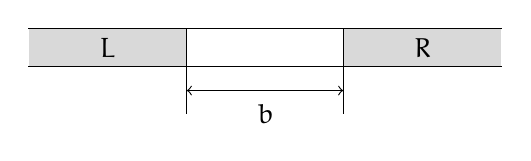
\begin{tikzpicture}
        \node[minimum width=2cm,fill=gray!30] (l) at (0,0) {$L$};
        \node[minimum width=2cm, right of=l, node distance=4cm, fill=gray!30] (r) {$R$};

        \draw[draw] (l.south west) -- (r.south east);
        \draw[draw] (l.north west) -- (r.north east);

        \draw[draw] (r.north west) -- ($ (r.south west)+(0,-.6) $);
        \draw[draw] (l.north east) -- ($ (l.south east)+(0,-.6) $);

        \draw[draw,<->] ($ (r.south west)+(0,-.3) $) -- ($ (l.south east)+(0,-.3) $);

        \node at ($ (l.south east)+(1,-.6) $) {$b$};
    \end{tikzpicture}
\end{center}
We will be interested in the speed of information transfer through the "buffer zone" from left to right, i.e., from area $L$ to area $R$. Suppose initially area $R$ is empty. What can be the complexity of string $R$ after $t$ steps from the start of operation? We will show that the complexity of $R$ does not exceed $(t\log m)/b + O(\log t)$, where $m$ is the number of states of the Turing machine. This can be explained informally: each state "carries" no more than $\log m$ bits of information, and in one step, information is transferred to one cell, so after $t$ steps, we will have transferred no more than $t\log m$ bits of information. We need to transfer information over a distance of $b$, which gives us $(t\log m) / b$.

\begin{theorem}
    Let a Turing machine with $m$ states be fixed. Then there exists a constant $c$ such that for any $b$ and for any computation with a buffer zone of $b$ (initially this zone and the tape to the right of it are empty, and the machine's head is to the left of the zone), the complexity of the right part of the tape $R(t)$ after $t$ steps of computation does not exceed
    $$\frac{t\log m}{b} + 4\log t + c.$$
\end{theorem}
\begin{proof}
    We will draw a boundary somewhere within the buffer zone, and each time the Turing machine's head crosses the boundary from left to right, we will record in which state it crossed it. We will call such a work protocol the \emph{trace} of the machine. Note that the trace can be used to reconstruct the operation of the machine to the right of the boundary—indeed, the behavior of the Turing machine to the right of the boundary depends only on the state in which the machine crossed the boundary and on what has already been written on the tape to the right of the boundary.

    To reconstruct $R(t)$, we need to specify the trace $S$, the number of steps $t' \le t$ that the Turing machine took to the right of the boundary, and the distance $b' < b$ from the boundary to $R$. We get
    $$
    K(R(t)) \le |\langle S, b', t'\rangle| + c
    \le |S|\cdot\log m + 2\log b + 2\log t + c
    \le |S|\cdot\log m + 4\log t + c.
    $$
    This inequality holds for any initial state and position of the boundary. If for the given $L$ we choose the \emph{shortest} trace for all possible boundary positions, then its length is guaranteed to be less than $t/b$ (there are $b + 1$ different boundary positions, and at each step only one of the possible boundaries is crossed, so the total length of the traces does not exceed $t$). Therefore, our estimate is valid for $|S| < t/b$.
\end{proof}

From this, we immediately obtain a quadratic lower bound for copying on a single-tape Turing machine. By copying, we mean the following process: initially, the tape contains some word $x \in \bitstr$, and to its right, the tape is empty. At the end of the Turing machine's operation, the tape should contain $xx$.

\begin{theorem}
    There exists a constant $\epsilon > 0$ such that for any $n$, there exists a word of length $n$ whose copying by machine $M$ takes at least $\epsilon n^2$ steps.
\end{theorem}
\begin{proof}
    For simplicity, let us assume that $n$ is even. Let $x$ be a word whose second half $u$ is incompressible (i.e., has complexity $\ge n/2$). We apply the theorem on the speed of information transfer, considering a buffer zone of length $n/2$ to the right of $x$.
    \begin{center}
        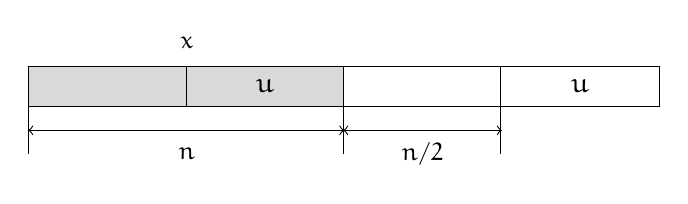
\begin{tikzpicture}[node distance=2cm]
            \node[minimum width=2cm,minimum height=.5cm,fill=gray!30] (a) at (0,0) {};
            \node[minimum width=2cm,minimum height=.5cm,right of=a, fill=gray!30] (b) {$u$};
            \node[minimum width=2cm,minimum height=.5cm,right of=b] (c)  {};
            \node[minimum width=2cm,minimum height=.5cm,right of=c] (d)  {$u$};

            \draw[draw] (a.south west) -- (d.south east);
            \draw[draw] (a.north west) -- (d.north east);

            \foreach \n in {a,d} {
                \draw[draw] (\n.north east) -- (\n.south east); }

            \foreach \n in {a,c,d} {
                \draw[draw] (\n.north west) -- ($ (\n.south west)+(0,-.6) $); }

            \draw[draw,<->] ($ (a.south west)+(0,-.3) $) -- ($ (b.south east)+(0,-.3) $);
            \draw[draw,<->] ($ (c.south west)+(0,-.3) $) -- ($ (c.south east)+(0,-.3) $);

            \node at ($ (a.north east)+(0,.3) $) {\small $x$};
            \node at ($ (a.south east)+(0,-.6) $) {\small $n$};
            \node at ($ (c.south)+(0,-.6) $) {\small $n/2$};
        \end{tikzpicture}
    \end{center}

    Assume the copying took $t$ steps, then the complexity of zone $R$ is at least $n/2$. On the other hand, by the previous theorem, the complexity of $R$ does not exceed $(t\log m)/b + 4\log t + c$, where $b = n/2$. Thus, we obtain that
    \[
    \frac{n}{2} \le \frac{t\log m}{b} + 4\log t + c.
    \]
    Assuming $t < n^2$ (otherwise, there is nothing to prove), we have $4\log t < 8\log n$. Hence,
    \[
    t \ge \frac{n^2}{4\log m} - O(n\log n).
    \]
    We can eliminate the second term if we choose $\epsilon$ slightly less than $1/(4\log m)$.
\end{proof}


\subsection{Algorithm for Adding Bit Numbers}
Let $\bar x = \overline{x_{n-1}\dotso x_0}$ and $\bar y = \overline{y_{n-1}\dotso y_0}$ be two $n$-bit numbers. We propose an algorithm for adding $\bar x$ and $\bar y$, which performs an average of $\log n$ operations (assuming that bitwise operations on $n$-bit numbers are done in $O(1)$).

The algorithm will be structured as follows.
\begin{itemize}
    \item First iteration.\\
    Compute $\bar z^{(1)}$: $z_i^{(1)} = x_i \oplus y_i$.\\
    Compute $\bar c^{(1)}$: $c_i^{(1)} = x_{i-1} \land y_{i-1}$ (carry vector).
    \item Iteration $k+1$.\\
    Compute $\bar z^{(k+1)}$: $z_i^{(k+1)} = z_i^{(k)} \oplus c_i^{(k)}$.\\
    Compute $\bar c^{(k+1)}$: $c_i^{(k+1)} = z_{i-1}^{(k)} \land c_{i-1}^{(k)}$.
\end{itemize}
Iterations stop when $\bar c^{(k)} = 0$.

Under what input can we perform $t$ iterations? It is claimed that this can only happen if $\bar x$ and $\bar y$ have continuous blocks of length $t$, where the corresponding bits are opposite, and there is a '$1$' following them.
\begin{center}
    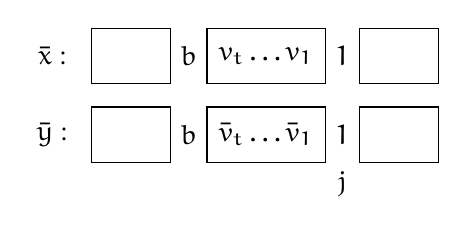
\begin{tikzpicture}[node distance=1cm]
        \tikzstyle{bigrect}=[draw, minimum width=1.5cm, minimum height=.7cm];
        \tikzstyle{rect}=[draw, minimum width=1cm, minimum height=.7cm];
        \node (y) at (0,0) {$\bar y:$};
        \node (x) at (0,1) {$\bar x:$};
        \node[rect,right of=x] (x1) {};
        \node[rect,right of=y] (y1) {};
        \node[right = 0mm of x1] (x2) {$b$};
        \node[right = 0mm of y1] (y2) {$b$};
        \node[right = 0mm of x2,bigrect] (x3) {$v_t\dotso v_1$};
        \node[right = 0mm of y2,bigrect] (y3) {$\bar v_t\dotso\bar v_1$};
        \node[right = 0mm of x3] (x4) {$1$};
        \node[right = 0mm of y3] (y4) {$1$};
        \node[right = 0mm of x4,rect]  {};
        \node[right = 0mm of y4,rect]  {};
        \node[below = 1mm of y4] {$j$};
    \end{tikzpicture}
\end{center}

Since $\bar x$ and $\bar y$ have a common block of bits of length $t$, we have
\[
K(\bar x \mid \bar y) \le (n - t - 2) + \underbrace{\log n}_{t} + \underbrace{\log n}_{j} + O(\log\log n).
\]
From this, it follows that $t \le n - K(\bar x \mid \bar y) + 2\log n + O(\log\log n)$. The average number of iterations in the algorithm can be estimated as
\[
\sum_t t \cdot [\text{fraction of pairs $(x, y)$ with a common block of length $t$}].
\]

We introduce the notation
$K(\bar x \mid \bar y) \le n - \underbrace{(t - 2\log n - O(\log\log n))}_{s}$ and we will call $s$ the \emph{defect of randomness}, i.e., $s = t - 2\log n + O(\log\log n)$ and $t \le s + 2\log n + O(\log\log n)$.

The fraction of pairs $(\bar x, \bar y)$ such that $K(\bar x \mid \bar y) = n - s$ is no more than $2^{-s + 1}$. We are interested in an asymptotic estimate, so we can assume that
\[
t \le s + 2\log n + O(\log\log n) \le s + 3\log n.
\]
Then the average number of iterations in the algorithm is at most
\[
\sum_s (s + 3\log n) \cdot 2^{-s + 1} = 6\log n \sum_s 2^{-s} + 2 \sum_s \frac{s}{2^s}
= O(\log n) + O(1).
\]
It is important to note that from $n - s \le n + O(1)$, we find that $-s \le O(1)$.

\subsection{Lovász Local Lemma}
Let a certain set of events $\{\seqn{A}{n}\}$ be given, and for each event, its probability is known as $\Pr[A_i] = \varepsilon_i$. What is the probability that none of these events occurs? There are two extreme cases.

\begin{itemize}
    \item If nothing is known about the nature of the events $\{A_i\}_{i=1}^n$, then
    \[
    \Pr[\overline{A}_1\land\overline{A}_2\land\dotsb\land\overline{A}_n]
    \ge 1 - \varepsilon_1 - \varepsilon_2 -\dotsb -\varepsilon_n.
    \]

    \item If all $\{A_i\}_{i=1}^n$ are independent collectively, then
    \[
    \Pr[\overline{A}_1\land\overline{A}_2\land\dotsb\land\overline{A}_n]
    = (1 - \varepsilon_1)\cdot(1 - \varepsilon_2) \cdot\dotso\cdot (1 - \varepsilon_n).
    \]
\end{itemize}

The Lovász Local Lemma provides an estimate in the intermediate case where the dependence between events is \emph{local}: each $A_i$ is dependent only on a relatively small number of \emph{neighbors}. We denote by $N(i)$ the set of neighbors of event $i$.

\begin{theorem}[Lovász Local Lemma] Let a set of $n$ events $\{\seqn{A}{n}\}$ be given, in which each event $A_i$ is independent of all events $A_j$, where $j \not\in N(i)$. If for each $i$, $\varepsilon_i < 1$ is chosen such that
    \[
    \Pr[A_i] \le \varepsilon_i \cdot \prod_{j \in N(i)} (1 - \varepsilon_j),
    \]
    then the probability that none of the events occur is
    \[
    \Pr[\overline{A}_1\land\overline{A}_2\land\dotsb\land\overline{A}_n]
    \ge (1 - \varepsilon_1)\cdot(1 - \varepsilon_2) \cdot\dotso\cdot (1 - \varepsilon_n).
    \]
\end{theorem}
\begin{proof}
    We start with a pair of simple statements. By the definition of conditional probability,
    \[
    \Pr[A \mid B] = \frac{\Pr[A \land B]}{\Pr[B]} \le \frac{\Pr[A]}{\Pr[B]}.
    \]
    This statement can be \emph{“relativized”}, i.e., we can add an additional condition $C$ to all probabilities:
    \begin{equation}\label{eq:lll:fact}
        \Pr[A \mid B \land C] \le \frac{\Pr[A \mid C]}{\Pr[B \mid C]}.
    \end{equation}

    We will prove the theorem by induction. The proof of the inductive step will consist of proving two statements.
    \begin{enumerate}
        \item For any $i$ and a set $J = \{\seqn{j}{k}\} \subset [n]$, with $i \not\in J$:
        \begin{equation}\label{eq:lll:ind1}
            \Pr[A_i \mid \overline A_{j_1} \land \overline A_{j_2} \land \dotsb \land \overline A_{j_k}] \le \varepsilon_i.
        \end{equation}
        \item For any disjoint sets $I, J \subset [n]$, $I = \{\seqn{i}{\ell}\}$, $J = \{\seqn{j}{m}\}$:
        \begin{equation}\label{eq:lll:ind2}
            \Pr[\overline A_{i_1} \land \overline A_{i_2} \land \dotsb \land \overline A_{i_\ell} \mid
            \overline A_{j_1} \land \overline A_{j_2} \land \dotsb \land \overline A_{j_m}] \ge
            (1 - \varepsilon_{i_1}) \cdot (1 - \varepsilon_{i_2}) \cdot \dotso \cdot (1 - \varepsilon_{i_\ell}).
        \end{equation}
    \end{enumerate}
    The relationship between these two statements will be formulated in the form of the following two lemmas.

    \begin{lemma}\label{lm:lll:l1}
        If inequality~\eqref{eq:lll:ind1} holds for all $k \le t$, then inequality~\eqref{eq:lll:ind2} holds for $\ell + m \le t + 1$.
    \end{lemma}
    \begin{proof}
        We will expand the probability on the left side of inequality~\eqref{eq:lll:ind2}
        using the “relativized” (i.e., with additional condition) definition of conditional probability $\Pr[A \land B \mid C] = \Pr[A \mid B \land C] \cdot \Pr[B \mid C]$
        (this formula will need to be applied $k$ times):
        \[
        \begin{aligned}
            \Pr[\overline A_{i_1} \land \overline A_{i_2} \land \dotsb \land \overline A_{i_\ell} \mid
            \overline A_{j_1} \land \overline A_{j_2} \land \dotsb \land \overline A_{j_m}] =\,
            &\Pr[\overline A_{i_1} \mid \overline A_{i_2} \land \dotsb \land \overline A_{i_\ell} \land
            \overline A_{j_1} \land \dotsb \land \overline A_{j_m}]\\
            \cdot&\Pr[\overline A_{i_2} \mid \overline A_{i_3} \land \dotsb \land \overline A_{i_\ell} \land
            \overline A_{j_1} \land \dotsb \land \overline A_{j_m}]\\
            &\ \vdots\\
            \cdot&\Pr[\overline A_{i_\ell} \mid
            \overline A_{j_1} \land \dotsb \land \overline A_{j_m}]\\
            \ge\,&(1 - \varepsilon_{i_1}) \cdot (1 - \varepsilon_{i_2}) \cdot \dotso \cdot (1 - \varepsilon_{i_\ell}).
        \end{aligned}
        \]
    \end{proof}

    \begin{lemma}\label{lm:lll:l2}
        If inequality~\eqref{eq:lll:ind2} holds for all $\ell$ and $m$ such that $\ell + m = t$, then inequality~\eqref{eq:lll:ind1} holds for $k = t$.
    \end{lemma}
    \begin{proof}
        If $J \cap N(i) = \emptyset$, then inequality~\eqref{eq:lll:ind1} holds, because
        $A_i$ is independent collectively with $\seqin{A}{i}{k}$. Otherwise, we introduce the following notations:
        \[N = \bigwedge_{j \in J \cap N(i)} \overline A_j,\quad
        F = \bigwedge_{j \in J \setminus N(i)} \overline A_j.
        \]
        In these notations, the left side of inequality~\eqref{eq:lll:ind1} can be rewritten as:
        \[
        \Pr[A_i \mid N \land F]
        \le \frac{\Pr[A_i \mid F]}{\Pr[N \mid F]}
        =   \frac{\Pr[A_i]}{\Pr[N \mid F]}
        \le \frac{\varepsilon_i \cdot \prod_{j \in N(i)} (1 - \varepsilon_j)}
        {\prod_{j \in J \cap N(i)} (1 - \varepsilon_j)} \le \varepsilon_i.
        \]
        Here, the first inequality is an application of inequality~\eqref{eq:lll:fact}; equality holds
        because $A_i$ is independent of $F$ (i.e., $A_i$ is independent of non-neighbors of $A_i$), and the second inequality
        follows directly from the condition of the theorem (numerator) and inequality~\eqref{eq:lll:ind2} for $\ell + m = k$ (denominator).
    \end{proof}

    Now we can describe how the induction will be structured. The base case of the induction is inequality~\eqref{eq:lll:ind1}
    for $k = 0$ (which follows from the condition of the theorem), which is the same as inequality~\eqref{eq:lll:ind2} for
    $\ell = 1$ and $m = 0$.
    Now we assume that we have already proven inequalities~\eqref{eq:lll:ind1} for $k < t$ and inequality~\eqref{eq:lll:ind2} for
    $\ell + m \le t$. We first apply lemma~\ref{lm:lll:l2} and obtain inequality~\eqref{eq:lll:ind1} for $k = t$.
    Then, using lemma~\ref{lm:lll:l1}, we will obtain inequality~\eqref{eq:lll:ind2} for $\ell + m = t + 1$.

    The proof is completed by the following observation: the local lemma of Lovász is a special case of
    inequality~\eqref{eq:lll:ind2} for $\ell = n$ and $m = 0$.
\end{proof}

\begin{corollary}[Lovász Local Lemma for the Symmetric Case]
    Suppose that in the condition of the Lovász Local Lemma it is additionally known that each event $A_i$
    has a probability of at most $p$ and a number of neighbors of at most $d$.
    Then, if \[ep(d + 1) \le 1,\] there is a positive probability that none of the events $A_i$ occurs.
\end{corollary}
\begin{proof}
    By Lovász's lemma, we need to choose $\varepsilon_i$ such that
    \[
    \Pr[A_i] \le p \le \varepsilon_i \cdot \prod_{j \in N(i)} (1 - \varepsilon_j).
    \]
    Let's take the same $\varepsilon$ for all events. Then it is enough to find $\varepsilon$ satisfying the condition
    \[
    p \le \varepsilon \cdot (1 - \varepsilon)^d.
    \]
    Consider the expression $(d\varepsilon) \cdot (1 - \varepsilon)^d$. If we sum all $d + 1$ factors (brackets), the total will be $d$. Thus, we need to maximize the product given a fixed sum of factors. The maximum occurs when all factors are equal, i.e., $d\varepsilon = 1 - \varepsilon$, and consequently $\varepsilon = 1/(d + 1)$.
    At this same value, the maximum of the original expression $\varepsilon \cdot (1 - \varepsilon)^d$ is achieved.
    We obtain
    \[
    p \le \frac{1}{d + 1} \cdot \biggl(1 - \frac{1}{d + 1}\biggr)^d.
    \]
    It remains to note that if $(1 + \frac{1}{d})^d < e$, then $(1 - \frac{1}{d + 1})^d > 1/e$ for $d \ge 1$.
\end{proof}

\begin{exercise}
    In each cell of a finite tape, we want to write a number from $1$ to $N$. However,
    for each boundary between cells, some pairs of numbers $(l,r)$ are forbidden,
    meaning that $l$ cannot be to the left of the boundary while $r$ is to the right. Prove
    that if for each boundary the proportion of forbidden pairs among all pairs is no greater
    than $4/27$, then the filling is possible.
\end{exercise}

\begin{exercise}
    Prove a similar result constructively and without using the local lemma of Lovász,
    if the set of bad pairs has measure less than $1/4$. (This shows that in this
    problem, the local lemma of Lovász does not provide an optimal answer.)
\end{exercise}

\begin{theorem}
    Let $\alpha < 1$ be some positive real number.
    Suppose that for each $n$, some binary words, totaling no more than $2^{\alpha n}$,
    are declared forbidden. Then there exists a number $N$ and an infinitely long sequence
    of zeros and ones that does not contain forbidden substrings longer than $N$.
\end{theorem}
\begin{proof}
    By compactness considerations, it is sufficient to prove the existence of arbitrarily long
    finite sequences without forbidden substrings.

    We will assume that the bits of the sequence are equally probable and independent. The occurrence
    of a forbidden sequence of length $n$ at a given position (on a given interval $I$)
    has a probability of $2^{(\alpha - 1)n}$, where $n$ is the length of the interval. As an estimate
    in Lovász's lemma for this event, we take $2^{(\beta - 1)n}$ for some
    $\beta \in (0,\alpha)$. We need to choose $\beta$ such that the condition of Lovász's lemma is satisfied.

    The neighbors of the event on interval $I$ are the events on intervals $J$ that overlap
    with $I$. Since the probabilities of events depend on the length, it is convenient to group
    the intervals by lengths. There are $n+k-1$ intervals of length $k$ overlapping with the given interval $I$
    of length $n$. For each of them, a factor of $(1-2^{(\beta - 1)k})$ appears on the right side of the estimate from Lovász's lemma, leading to
    \[
    \bigl(1-2^{(\beta - 1)k}\bigr)^{n+k-1}.
    \]
    Now we multiply this over all $k$ starting from some $N$. Thus,
    for the application of Lovász's lemma, we need that
    \[
    2^{(\alpha - 1)n} \le 2^{(\beta - 1)n} \cdot \prod_{k \ge N}
    \bigl(1-2^{(\beta - 1)k}\bigr)^{n+k-1}.
    \]
    (In this formula, the right side also accounts for the interval $I$ when $n=k$,
    but this only decreases the right side.) We will show that a stronger inequality holds: we will roughly estimate $n+k - 1 \le nk$ (i.e., we will reduce the numbers in the product),
    take the $n$-th root, and move $2^{\beta - 1}$ to the left.
    \[
    2^{(\alpha - \beta)} \le \prod_{k \ge N} \bigl(1-2^{(\beta - 1)k}\bigr)^k.
    \]
    We apply Bernoulli's inequality to the right side ($(1 - x)^k \ge 1 - kt$) — this will further strengthen the inequality. We obtain
    \[
    2^{(\alpha - \beta)} \le 1 - \sum_{k \ge N} k2^{(\beta - 1)k}.
    \]
    The series on the right converges for $\beta < 1$, and the left side is less than $1$
    for $\alpha < \beta$. Thus, for $\alpha$, we can choose $\beta < \alpha$
    and sufficiently large $N$ such that this inequality holds, which means the original weaker inequality also holds. Therefore, we can apply
    the local lemma of Lovász for words of length at least $N$.

    To obtain an infinite good word, we will construct it iteratively.
    We start with some good word of length $1$, which has infinitely many
    good extensions (it is easy to see that such a word exists). We will gradually add
    one symbol at a time so that the resulting word also has infinitely many
    good extensions (it is easy to see that at each step, at least one of the symbols will fit).
\end{proof}

\begin{exercise}[Levin's Lemma]
    Let $\alpha < 1$ be some positive real number.
    Then there exists an infinite sequence of zeros and ones,
    in which all substrings of sufficiently large length $n$ have complexity
    of at least $\alpha n$.
\end{exercise}

\begin{exercise}\label{ex:lll:rects}
    Prove a two-dimensional analog of the previous theorem: it is possible to fill an infinite
    grid with zeros and ones such that any rectangle of sufficiently large area is not forbidden, if for each
    rectangle of area $k$, no more than $2^{\alpha k}$ forbidden ones are chosen,
    where $\alpha < 1$.
\end{exercise}

Let $w=w_0w_1w_2\dotso$ be an infinite sequence. For any finite
set $F\subset\mathbb{N}$ of indices, we denote by $w(F)$ the word composed
of the symbols of $w$ at the positions specified by $F$ (in increasing order of indices). Consider a pair $(F, X)$,
where $F$ is a finite set of indices, and $X$ is a word of length $|F|$. We say that
the sequence $w$ is forbidden by the pair $(F,X)$ if $w(F) = X$. Such pairs
are called \emph{forbiddances}, and the number of elements in $F$ is called the \emph{size of the forbiddance}. A forbiddance \emph{covers} the indices in $F$.

\begin{theorem}\label{thm:lll:subseq}
    Let $\alpha < 1$ be some positive real number and let
    $\{(F,X)\}$ be a set of forbiddances, where for any index $i$
    and number $n$, there are no more than $2^{\alpha n}$ forbiddances of size $n$
    that cover $i$. Then there exists a number $N$ and a sequence
    that is not forbidden by any forbiddance of size greater than $N$.
\end{theorem}
\begin{proof}
    Similarly to the previous theorem, we will prove this statement for
    finite sequences and then use compactness.

    We apply Lovász's lemma to the violations of forbiddances.
    The probability of violating a forbiddance of size $n$ is $2^{-n}$.
    For a forbiddance of size $n$, we take $\varepsilon_i = 2^{-\beta n}$,
    where $\beta$ is some constant greater than $\alpha$.

    The neighbors of a forbiddance will be the forbiddances that intersect with it (covering a common index).
    For Lovász's lemma, we need to take a forbiddance of size $n$ and check that $2^{-n}$ is not greater than $2^{-\beta n}$,
    multiplied by the product of factors $(1-2^{-\beta m})$ for all forbiddances intersecting with the given one.

    We will split the product into parts corresponding to the different intersection points.
    There are a total of $n$ such possible points. Furthermore, at each point, we will group the factors
    by sizes. Then for a given point and a given size of forbiddance $m$, we will obtain no more than
    $2^{\alpha m}$ factors of the form $(1-2^{-\beta m})$. Thus, we need to verify the inequality
    \[
    2^{-n}\le 2^{-\beta n}\cdot\prod_{m\ge N} (1-2^{-\beta m})^{2^{\alpha m}n}.
    \]
    Taking the $n$-th root, we have
    \[
    2^{\beta-1}\le \prod_{m\ge N} (1-2^{-\beta m})^{2^{\alpha m}}.
    \]
    By Bernoulli's inequality, this holds if
    \[
    2^{\beta-1}\le 1 - \sum_{m\ge N} 2^{\alpha m}\cdot 2^{-\beta m}.
    \]
    Since the left-hand side is less than $1$, and the series on the right converges, for
    sufficiently large $N$, this inequality holds.

    Analogously to the previous theorem, we can construct an infinite sequence
    that does not violate forbiddances of large size (we first need to choose $\beta$, then
    sufficiently large $N$, and apply Lovász's lemma to sequences
    of arbitrary length).
\end{proof}

\begin{corollary}
    Let $\alpha < 1$ be some positive real number.
    There exists a sequence $w$ and a constant $N$ such that
    \[
    \max_{t\in F} K(F,w(F) \mid t) \ge \alpha |F|
    \]
    for all $F\subset\mathbb{N}$ containing at least $N$ elements.
\end{corollary}

\begin{remark}
    In this corollary, the left side of the inequality in the Kolmogorov complexity concerning $w(F)$
    somehow includes $F$. This is because the complexity of a subsequence
    can be "encoded" in the set of indices: for example, in $F$ we can write
    the indices of zeros within $w$, making $K(w(F)) = O(1)$. The maximum conditional complexity
    on the left arises because we want to be able to "shift" the set of indices $F$
    along the sequence, so $t$ in this case serves as something like a "reference point."
    In this formulation, for example, the set of indices $\{2,4,6\}$ will
    have the same complexity as $\{i, i+2, i+4\}$ for any $i$, even if the complexity of $i$ is large.
\end{remark}

Note that from this it follows, in particular, that any finite set $F$
of size at least $N$ has an element $t$ for which
\[
K(w(F) \mid F, t) \ge \alpha |F| - 2K(F \mid t).
\]
If we omit $t$ from the left side, we get that for any sufficiently large $F$
\[
K(w(F) \mid F) \ge \alpha |F| - 2\max_{t\in F} K(F \mid t).
\]
If we consider the indices arranged in a plane, and take rectangles as $F$,
then the term subtracted on the right will be logarithmic and can be compensated by
$\alpha$. This leads to the statement of exercise~\ref{ex:lll:rects}.
\begin{proof}
    We apply theorem~\ref{thm:lll:subseq}, where for the forbiddances $(F,Z)$ the inequality
    $K(F,Z\mid t) < \alpha|F|$ holds for all $t\in F$. Thus, for
    each index $t$, the number of forbiddances of size $k$ that include $t$
    does not exceed $2^{\alpha k}$.
\end{proof}

\subsubsection{``Effective'' proof of Lovász's lemma}
All previous discussions about Lovász's lemma were non-constructive—we proved
the existence of certain objects but did not explain how to find them. Moreover,
in our proofs, a ``good'' object could have an exponentially small
probability, making it unlikely to randomly ``guess'' it within a
reasonable (polynomial) number of attempts.

In this section, we will propose a very simple probabilistic algorithm
that, with constant probability, will find a ``good'' object in polynomial time. We will consider the application of the algorithm to
a specific problem. Suppose we need to find a binary word, given
some set of forbiddances; in other words, we need to find a satisfying assignment for a CNF formula. We will select a random set of values for the variables. Some
fraction of forbiddances will be violated in this case. We will take some
forbiddance and choose values for the variables involved in it again.
Most likely, this forbiddance will be satisfied with the new variable values,
but some other forbiddances may be violated. If so, we will repeat the process
for the newly violated forbiddances. And so on. Remarkably,
this simple algorithm leads to the desired outcome.

For simplicity, we will assume that all forbiddances are of the same size.
Let the CNF contain $n$ variables and $N$ clauses of size $m$. We will consider clauses that share a common variable with the given one as neighbors. Suppose that
each clause has no more than $t$ neighbors. If $t$ is small,
then by Lovász's lemma, this formula is satisfiable.

Since all clauses are of the same size, it is reasonable to choose
the same $\varepsilon$ in Lovász's lemma for all events. Then we must satisfy the following inequality:
\[
2^{-m} \le \varepsilon(1-\varepsilon)^t.
\]
The right side is maximized at $\varepsilon = 1/(t+1)$, but for simplicity, we will set $\varepsilon = 1/t$.
Thus, we have $2^{-m} \le (1-1/t)^t/t \approx 1/et$, meaning satisfiability is guaranteed when $t \le 2^m/e$.
In the constructive proof, we will need a stronger condition $t \le 2^m/8$.

\begin{theorem}[Moser, Tardos, 2009]
    There exists a probabilistic algorithm that finds a satisfying assignment for any formula in
    CNF with $n$ variables and $N$ clauses of size $m$, each having no more than $2^m/8$
    neighbors, in polynomial time in terms of $n + N$ with a probability of at least $1/2$.
\end{theorem}

\begin{proof} We will assume that there is a fixed order on the clauses.
    The algorithm will use a recursive procedure $\mathrm{Fix}(d)$:
    \begin{quote}
        choose random values for the variables $x$;\\
        for all clauses $d$ of the formula:\\
        \mbox{}\quad if $d(x) = 0$, then call $\mathrm{Fix}(d)$.
    \end{quote}
    For the algorithm to be correct, the procedure $\mathrm{Fix}$
    must not violate the satisfiability of the clauses that we have already considered
    (i.e., by the time we call $\mathrm{Fix}(d)$, all clauses to the left of $d$ must already
    be satisfied and must remain satisfied after the call to $\mathrm{Fix}(d)$).

    The body of the procedure $\mathrm{Fix}(d)$:
    \begin{quote}
        update $x$, choosing random values for all variables in $d$;\\
        for all neighbors $d'$ of clause $d$:\\
        \mbox{}\quad if $d'(x) = 0$, then call $\mathrm{Fix}(d')$.
    \end{quote}
    We will assume that the clause is a proper neighbor, so we do not need to
    separately consider the case where the new variable values for $d$
    are the same as the previous ones (i.e., the clause is not satisfied again).
    The correctness of $\mathrm{Fix}$ follows from its definition—if it completes,
    it cannot make other clauses unsatisfied, as it only modifies
    the variables that are present in $d$.

    It remains to show that with high probability, the process will complete in polynomial time.
    Note that random bits in this algorithm are only used to choose initial
    values for the variables ($n$ bits) and at each iteration of $\mathrm{Fix}$—to choose new
    values for the variables of the clause ($m$ bits).

    We will use the following observation: all random bits used up to this
    moment in the algorithm can be reconstructed from the current values of the variables and
    the list of clauses for which the procedure $\mathrm{Fix}$ was called. Indeed,
    if at some points in time the procedure $\mathrm{Fix}(d)$ was called,
    we can reconstruct the values of the variables in $d$, as the clause is not satisfied
    only for one specific setting of the variables. Then we can start reconstructing the events
    from the end and recover all bits used by the algorithm.

    Suppose that at this moment $k$ calls to $\mathrm{Fix}$ have occurred, i.e., the algorithm
    has used $n + km$ random bits. To reconstruct them, it is sufficient to know:
    \begin{enumerate}
        \item the current values of the variables,
        \item the indices of the clauses for which $\mathrm{Fix}$ was called from the main algorithm,
        \item which calls to $\mathrm{Fix}$ were made recursively for each of the clauses.
    \end{enumerate}
    For the first, $n$ bits are required; for the second, no more than $N$ bits (the indices of the clauses can
    be specified using a bitmask). For the third, we need to describe the tree of recursive calls.
    We will encode the tree as follows: when making a recursive call from $d$, it is sufficient to specify
    the index of the neighbor for which we are calling, which requires $\log t$ bits. Additionally,
    we need to distinguish between situations where a recursive call occurs in $\mathrm{Fix}$
    (moving down the call tree) and when exiting the procedure (moving up the call tree).
    Thus, for each transition, we will add one bit: $0$ if we exit the procedure,
    $1$ if we move to a neighbor, and the next $\log t$ bits will be the index of the neighbor.

    In total, for each vertex of the call tree, we will spend $\log t + 2$ bits. This yields $N + n + k\cdot(\log t + 2)$.
    With a probability of $1/2$, the random bits have maximum Kolmogorov complexity, i.e.,
    \[
    n+k\cdot m - 1 \le K(\text{random bits}) \le N + n + k\cdot(\log t + 2) + c,
    \]
    which gives an upper bound on $k$, since $\log t + 2 = \log (2^m/8) + 2 = m - 1$.
    Therefore, we have $k \le N + c + 1$, where $c$ is a constant.
\end{proof}

\newpage
%%%%%%%%%%%%%%%%%%%%%%%%%%%%%%%%%%%%%%%%%%%%%%%%
\begin{thebibliography}{9}
    \bibitem{veresch12} Н.К. Верещагин, Е.В. Щепин. \emph{Информация, кодирование, предсказание}, МЦНМО, 2012.

    \bibitem{veresch17} Н.К. Верещагин. \emph{Коммуникационная сложность}, Computer Science клуб, 2017.
        \url{http://compsciclub.ru/courses/communicationcomplexity/2017-spring/}

    \bibitem{romaschcsclub} А.Е. Ромащенко. \emph{Введение в теорию информации,} Computer Science клуб, 2015.
        \url{http://compsciclub.ru/courses/informationtheory/2015-spring/}

    \bibitem{romaschnotes} А.Е. Ромащенко. \emph{Краткий конспект лекций курса ``Введение в теорию информации'',} 2014.
        \url{http://www.mccme.ru/~anromash/courses/lecture-notes-it-2014.pdf}

    \bibitem{kolmbook12} В.А. Успенский, Н.К. Верещагин, А.Шень. \emph{Введение в колмогоровскую сложность}. МЦНМО, 2012.

    \bibitem{shen08} А. Шень. \emph{Алгоритмическая теория информации,} Computer Science клуб, 2008.
        \url{http://compsciclub.ru/courses/algo-information-theory/2008-autumn/}

    \bibitem{BB94} M. L. Bonet, S. R. Buss. \emph{Size-depth tradeoffs for Boolean formulae.} Information Processing Letters, 49(3), 151-155, 1994.

    \bibitem{DMWW12} D. Gavinsky, O. Meir, O. Weinstein, A. Wigderson. \emph{Toward better formula lower bounds:
    an information complexity approach to the KRW composition conjecture.} STOC 2014.

    \bibitem{KRV18} T.Kaced, A.E. Romashchenko, N.K.Vereshchagin, \emph{A Conditional Information Inequality and Its Combinatorial Applications}.
    {{IEEE} Trans. Information Theory}, 2018.

    \bibitem{NK97} E. Nisan, N. Kushilevitz. \emph{Communication complexity}, 1997.

    \bibitem{rao10} A. Rao. \emph{Notes for CSE533: Information Theory in Computer Science}, 2010. \\ \url{https://homes.cs.washington.edu/~anuprao/pubs/CSE533Autumn2010/}

\end{thebibliography}


\end{document}

% vim: set tw=120:
